% Remarks:
% Podles sphere can be defined as an algebra in $\Rep(SU_q(2))$. Hence, it should make sense as an algebra under the forgetful functor to SU_q(2)-dynamical. By duality for coideals, the same should hold for passage to SU_q(1,1) in fact...
%
% link with article `Racah - Wigner quantum 6j Symbols, Ocneanu Cells for AN diagrams and quantum groupoids' by Coquereaux?
% Ref to Schauenburg that face algebras are weak Hopf algebras
% Thanks to Makoto, Piotr (?), Leonid
% Cf. Enocks quantum groupoids of compact type
% Donin, J.(IL-BILN); Mudrov, A.(IL-BILN), Quantum groupoids and dynamical categories. 
% Leonid, cf. talk www.fields.utoronto.ca/programs/scientific/13-14/.../Vainerman.pdf
% Stokman vertex irf babelon cocycle twist
% Level 2 Hecke algebras Brundan
% Concerning locally unital algebras ask J. Vercruysse on recent work 
% Say construction groupoids from forgetful functors on temperley-Lieb already in Enock-Ostrik remark
\documentclass[11pt]{article}

\usepackage{hyperref}
\usepackage{fixme}
\usepackage{mathrsfs}
\usepackage[a4paper]{geometry}
\usepackage{amssymb, amsthm, amsfonts, amsxtra, amsmath}
\usepackage{latexsym}
\usepackage{mathabx}
\usepackage{enumitem}
%\usepackage[all]{xy}
%\usepackage{graphics}
\usepackage{pdfpages}
\usepackage{epic}
\usepackage{parskip} % paragraphs have no indents and vertical spacings inbetween
\makeatletter % need this to avoid the conflict between amsthm and parskip
\def\thm@space@setup{%
  \thm@preskip=\parskip \thm@postskip=0pt
}
\makeatother

%\theoremstyle{change}

\newcommand{\co}{\mathrm{co}}
\newcommand{\Corep}{\mathrm{Corep}}
\newcommand{\sff}{\textrm{s.f.~}}
\newcommand{\sfs}{\mathrm{sfs}}
\newcommand{\sfd}{\mathrm{sfd}}
\DeclareMathOperator{\Hom}{Hom}
\DeclareMathOperator{\img}{img}

\DeclareMathOperator{\id}{id}
\DeclareMathOperator{\ext}{\mathrm{e}}
\DeclareMathOperator{\can}{\mathrm{can}}
\DeclareMathOperator{\op}{\mathrm{op}}
\DeclareMathOperator{\fin}{\mathrm{f}}
\DeclareMathOperator{\Pol}{\mathrm{P}}
\DeclareMathOperator{\End}{\mathrm{End}}
\DeclareMathOperator{\Par}{\mathrm{Par}}
\DeclareMathOperator{\reg}{\mathrm{reg}}
\DeclareMathOperator{\sgn}{\mathrm{sgn}}
\DeclareMathOperator{\Zz}{\mathrm{Z}}
\DeclareMathOperator{\Ran}{\mathrm{Ran}}
\DeclareMathOperator{\hol}{\mathrm{hol}}
\DeclareMathOperator{\Ind}{\mathrm{Ind}}
\DeclareMathOperator{\Ker}{\mathrm{Ker}}
\DeclareMathOperator{\Char}{\mathrm{Char}}
\DeclareMathOperator{\dyn}{\mathrm{dyn}}
\DeclareMathOperator{\Spec}{\mathrm{Spec}}
\DeclareMathOperator{\adj}{\mathrm{adj}}

\newcommand{\Circt}{\underset{I}{\mathop{\ooalign{$\ovoid$\cr\hidewidth\raise-.05ex\hbox{$\scriptstyle\mathsf T\mkern3.5mu$}\cr}}}} % Woronowicz style tensor product, USUAL SIZE
\newcommand{\Circtv}[1]{\underset{#1}{\mathop{\ooalign{$\ovoid$\cr\hidewidth\raise-.05ex\hbox{$\scriptstyle\mathsf T\mkern3.5mu$}\cr}}}} % Woronowicz style tensor product, USUAL SIZE
\newcommand{\smCirct}{\mathop{\ooalign{$\scriptstyle\ovoid$\cr\hidewidth\raise-.05ex\hbox{$\scriptscriptstyle\mathsf T\mkern2.8mu$}\cr}}}  % Woronowicz style tensor product, SCRIPT SIZE

\newcommand{\nc}{\R}
\newcommand{\g}{\mathfrak{g}}
\newcommand{\h}{\mathfrak{h}}

\newcommand{\kk}{\mathfrak{k}}
\newcommand{\ttt}{\mathfrak{t}}
\newcommand{\p}{\mathfrak{p}}
\newcommand{\n}{\mathfrak{n}}
\newcommand{\llll}{\mathfrak{l}}
\newcommand{\uu}{\mathfrak{u}}
\newcommand{\bb}{\mathfrak{b}}
\newcommand{\q}{\mathfrak{q}}
\newcommand{\su}{\mathfrak{su}}
\newcommand{\ssl}{\mathfrak{sl}}
\newcommand{\SSL}{\mathrm{SL}}
\newcommand{\so}{\mathfrak{so}}
\newcommand{\spp}{\mathfrak{sp}}
\newcommand{\G}{\mathbb{G}}
\newcommand{\e}{\mathfrak{e}}
\newcommand{\s}{\mathfrak{s}}
\newcommand{\C}{\mathbb{C}}
\newcommand{\R}{\mathbb{R}}
\newcommand{\Z}{\mathbb{Z}}
\newcommand{\N}{\mathbb{N}}
\newcommand{\X}{\mathbb{X}}
\newcommand{\Y}{\mathbb{Y}}
\newcommand{\Ss}{\mathbb{S}}
\newcommand{\ZZ}{\mathscr{Z}}
\newcommand{\ad}{\mathrm{ad}}
\newcommand{\Hsp}{\mathcal{H}}
\newcommand{\qn}[2]{\lbrack #1 \rbrack_{#2}}
\newcommand{\fqn}[2]{\lbrack #1 \rbrack_{#2}!}
\newcommand{\bqn}[3]{\left\lbrack \begin{array}{c} \!#1\! \\ \!#2\! \end{array}\right\rbrack_{#3}}
\newcommand{\Tr}{\mathrm{Tr}}
\newcommand{\RR}{\mathcal{R}}
\newcommand{\rd}{\mathrm{d}}
\newcommand{\res}{\mathrm{res}}
\newcommand{\cop}{\mathrm{cop}}
\newcommand{\opp}{\mathrm{op}}
\newcommand{\coop}{\mathrm{coop}}
\newcommand{\Rm}{\mathcal{R}}
\newcommand{\wt}{\mathrm{wt}}
\newcommand{\Ad}{\mathrm{Ad}}
\newcommand{\CatC}{\mathcal{C}}
\newcommand{\CatD}{\mathcal{D}}
\newcommand{\Corr}{\mathrm{Corr}}
\newcommand{\Hilb}{\mathrm{Hilb}}
\newcommand{\Star}[2]{{}_{#1}\!*_{#2}}
\newcommand{\vot}{\bar{\otimes}}
\newcommand{\A}{\mathcal{B}}
\newcommand{\Aa}{\mathscr{B}}
\newcommand{\Mor}{\mathrm{Mor}}
\newcommand{\alg}{\mathrm{alg}}
\newcommand{\Gg}{\mathscr{G}}
\newcommand{\ev}{\mathrm{ev}}
\newcommand{\Rtimes}{\underset{\R}{\times}}
\newcommand{\Rb}{\R^{\bullet}}
\newcommand{\vtimes}{\bar{\otimes}}
\newcommand{\Rr}{\mathscr{R}}
\newcommand{\Tt}{\mathscr{T}}
\newcommand{\Fun}{\mathrm{Fun}}
\newcommand{\Ff}{\Fun_{\fin}}
%\newcommand{\fin}{\mathrm{fin}}
\newcommand{\iitimes}{\underset{I}{\otimes}}
\newcommand{\itimes}{\underset{I^2}{\otimes}}
\newcommand{\osum}[1]{\underset{#1}{\sum}^{\oplus}}
\newcommand{\osumc}[1]{\underset{#1}{\sum}^{\bar{\oplus}}}
\newcommand{\oplusc}{\bar{\oplus}}
\newcommand{\wDelta}{\widetilde{\Delta}}
\newcommand{\f}{\mathrm{fin}}
%\newcommand{\Hilb}{\mathrm{Hilb}}
\newcommand{\Rho}{\mathrm{P}}
\newcommand{\Rep}{\mathrm{Rep}}
\newcommand{\DA}{\mathcal{A}}
%\newcommand{\Circt}{\mathop{\ooalign{$\ovoid$\cr\hidewidth\raise-.05ex\hbox{$\scriptstyle\mathsf T\mkern3.5mu$}\cr}}} % Woronowicz style tensor product, USUAL SIZE
\newcommand{\CoRep}{\mathrm{Corep}}
\newcommand{\even}{\mathrm{even}}
\newcommand{\odd}{\mathrm{odd}}
\newcommand{\fd}{\mathrm{fd}}

\newcommand{\GrHA}[3]{#1{\begin{pmatrix} #2,  #3\end{pmatrix}}}% Horizontal grading ordinary style, with argument
\newcommand{\Grs}[3]{#1{\begin{pmatrix} #2,  #3\end{pmatrix}}}

\newcommand{\GrDA}[3]{\;{}_{\;#2}#1_{#3}} % Horizontal grading bottom style, with argument
%\newcommand{\Grd}[3]{\;{}_{\;#2}#1_{#3}}

\newcommand{\GrVA}[3]{#1{\tiny {\begin{pmatrix} #2\\#3\end{pmatrix}}}} % Vertical grading ordinary style, with argument
\newcommand{\Grt}[3]{#1{\tiny {\begin{pmatrix} #2\\#3\end{pmatrix}}}} 

\newcommand{\GrRA}[3]{#1^{#2}_{#3}} % Vertical grading right style, with argument

\newcommand{\Unit}{\mathbf{1}}
\newcommand{\UnitC}[2]{\mathbf{1}\!\begin{pmatrix} #1 \\ #2\end{pmatrix}} 
\newcommand{\Grru}[2]{{\tiny \begin{pmatrix} #1 \\ #2\end{pmatrix}}}

\newcommand{\eGr}[5]{#1{{\tiny \begin{pmatrix} #2 \quad #3 \\ #4 \quad #5\end{pmatrix}}}}

\newcommand{\pma}[4]{\begin{pmatrix} #1 \quad #2 \\ #3 \quad #4\end{pmatrix}}
\newcommand{\pmat}[4]{{\tiny \begin{pmatrix} #1 \quad #2 \\ #3 \quad #4\end{pmatrix}}}

\newcommand{\UT}[2]{#1{\tiny #2 }}
\newcommand{\Gr}[5]{\;{}^{\;#2}_{#4}#1_{#5}^{#3}}%TODO: better typesetting
%\newcommand{\Gr}[5]{\UT{#1}{\begin{pmatrix} #2\quad #3 \\ #4 \quad #5\end{pmatrix}}}
%\newcommand{\Gr}[5]{\UT{#1}{\begin{pmatrix} \, #2\;\\ #3 \qquad #4 \\ \,#5\;\end{pmatrix}}}
\newcommand{\Grl}[3]{\;{}^{\;#2}_{#3}#1}%TODO: better typesetting
\newcommand{\Gru}[3]{{}^{\;#2}#1^{#3}}
\newcommand{\Grd}[3]{{}_{\;#2}#1_{#3}}
\newcommand{\gr}[5]{\;{}^{\;#2}_{#4}#1_{#5}^{#3}}%TODO: better typesetting
\newcommand{\eGrr}[3]{#1_{{\tiny \left(#2, #3\right)}}}
\newcommand{\eGrt}[4]{#1{{\tiny \begin{pmatrix} #2 \\ #3 \\ #4 \end{pmatrix}}}}
\newcommand{\Grr}[4]{\begin{pmatrix}#1 \quad #2\\#3&#4\end{pmatrix}}

\newcommand{\Grss}[3]{\UT{#1}{\begin{pmatrix} #2 \; #3\end{pmatrix}}}
\newcommand{\Grb}[7]{\UT{#1}{\begin{pmatrix} #2\quad #3 \\ #4 \quad #5\\ #6 \quad #7\end{pmatrix}}}
\newcommand{\un}[2]{e{{\tiny \begin{pmatrix}#1\\ #2\end{pmatrix}}}}
\newcommand{\unn}[3]{e{{\tiny \begin{pmatrix}#1\\ #2\\#3\end{pmatrix}}}}

\newcommand{\wmult}{\cdot}
\newcommand{\bmult}{*}
\newcommand{\wmate}{\rightarrow}% Change this to source/target notation l(eft) r(ight)
\newcommand{\bmate}{\downarrow}% Change this to source/target notation u(p) d(own)

\newcommand{\aste}[1]{\underset{#1}{\ast}}

\newcommand{\Vv}{\mathcal{V}}

\newcommand{\dT}{\dot T}

\newtheorem{Theorem}{Theorem}[section]
\newtheorem{Lem}[Theorem]{Lemma}
\newtheorem{Prop}[Theorem]{Proposition}
\newtheorem{Cor}[Theorem]{Corollary}

\theoremstyle{definition}
\newtheorem{Def}[Theorem]{Definition}
\newtheorem{Rem}[Theorem]{Remark}
\newtheorem{Exa}[Theorem]{Example}
\newtheorem{Not}[Theorem]{Notation}
\newtheorem{Que}[Theorem]{Question}
\newtheorem{Con}[Theorem]{Conjecture}


%%%%%%%%%%%%%%%%%%%
% Notation for Section 4
\newcommand{\LGtwo}{L^{2}(\mathscr{G})}
\newcommand{\LGinf}{L^{\infty}(\mathscr{G})}
\newcommand{\CrG}{C^{r}_{0}(\mathscr{G})}
\newcommand{\vnDelta}{\overline{\Delta}}
\newcommand{\vnE}{\overline{E}}
\newcommand{\astrl}{\underset{l^{\infty}(I)}{_{\rho}\ast_{\lambda}}}
\newcommand{\otimesrl}{\underset{\nu{}}{_{\rho}\otimes_{\lambda}}}
\newcommand{\vnphi}{\overline{\phi}}
\newcommand{\vnphic}[2]{\vnphi{#1\choose #2}}

\date{}


\numberwithin{equation}{section}

\begin{document}
\title{Partial compact quantum groups, compact quantum homogeneous spaces and the dynamical quantum $SU(2)$ group}

\author{Kenny De Commer\thanks{Department of Mathematics, Vrije Universiteit Brussel, VUB, B-1050 Brussels, Belgium, email: {\tt kenny.de.commer@vub.ac.be}}
\and Thomas Timmermann\thanks{University of M\"{u}nster}}

\maketitle

% Terminology `compact' might have to be adapted if we work with infinitely many objects.
\begin{abstract}
\noindent Compact quantum groups of face type, as introduced by T. Hayashi, form a class of quantum groupoids with a classical, finite set of objects. We generalize Hayashi's definition to allow for an infinite set of objects, and call the resulting objects partial compact quantum groups. We then show how any quantum homogeneous space of an ordinary compact quantum group leads to a partial compact quantum group. In particular, when this construction is applied to the non-standard Podle\'{s} spheres, we obtain partial compact quantum groups which are operator algebraic versions of the dynamical quantum $SU(2)$-group as studied by Etingof-Varchenko and Koelink-Rosengren.% References ok?
\end{abstract}


%\emph{Keywords}:

%AMS 2010 \emph{Mathematics subject classification}:


%17B37: Quantum groups, quantized enveloping algebras
%20G42: quantized function algebras
%46L65: Functional analysis, deformations, quantizations
%81R50: Quantum groups and related algebraic methods
%16T05: Hopf algebras and their applications
%16T10: Bialgebras
%16T15: Coalgebras and comodules; corings
%46L08  $C^*$-modules


\section{Compact quantum groups of face type}

We generalize Hayashi's definition of a compact quantum group of face type \cite{Hay1} to the case where the commutative base algebra is no longer finite-dimensional. We will present two approaches, based on \emph{partial bialgebras} and \emph{weak multiplier bialgebras} \cite{Boh1}. The first approach is piecewise and concrete, but requires some bookkeeping. The second approach is global but more abstract. As we will see from the general theory and the concrete examples, both approaches have their intrinsic value.

%\begin{Not} If $I$ is a set, we write $\Fun_{\fin}(I)$ for the algebra of \emph{finitely supported} $\C$-valued functions on $I$\\

%We write $\Fun(I)$ for the algebra of \emph{all} $\C$-valued functions on $I$. %We will always suppose that $I$ is at most countable.
%\end{Not}

% Notation $I$ ok, or better $O$?

Let $I$ be a set. We consider $I^2=I\times I$ as the pair groupoid with $\wmult$ denoting composition. That is, an element $K=(k,l)\in I^2$ has source $K_l = k$ and target $K_r=l$, and if $K=(k,l)$ and $L=(l,m)$ we write $K\wmult L = (k,m)$. %For general $K,L\in I^2$, we write the property `$K$ and $L$ are composable' as $K\wmate L$. 

\begin{Def} A \emph{partial algebra} $\mathscr{A}=(\mathscr{A},M)$ (over $\C$) is a small $\C$-linear category, that is, a set $I$ (the object set) together with %Change partial by face? Partial algebra might have distinct meaning
\begin{itemize}
\item[$\bullet$] for each $K=(k,l)\in I^2$ a vector space $A(K) = \Grs{A}{k}{l}=\!\!\GrDA{A}{k}{l}$ (possibly the zero vector space),
\item[$\bullet$] for each $K,L$ with $K_r = L_l$ a multiplication map \[M(K,L):A(K) \otimes A(L)\rightarrow A(K\cdot L),\qquad a\otimes b \mapsto ab\]  and 
\item[$\bullet$] elements $\Unit(k) = \Unit_k \in \Grs{A}{k}{k}$ (the units), % or the local units?
\end{itemize}
such that the obvious associativity and unit conditions are satisfied. 

By \emph{$I$-partial algebra} will be meant a partial algebra with object set $I$.
\end{Def}


\begin{Rem} For the moment we will allow the local units $\Unit_k$ to be zero. When none of the units are zero, we will call the partial algebra \emph{connected}. 
\end{Rem}

Let $\mathscr{A}$ be an $I$-partial algebra. We define $A(K\wmult L)$ to be $\{0\}$ when $K_r\neq L_l$, and we then let $\Grs{M}{K}{L}$ be the zero map.

\begin{Def} The \emph{total algebra} $A$ of an $I$-partial algebra $\mathscr{A}$ is the vector space \[A = \oplus_{K\in I^2} A(K)\] endowed with the unique multiplication whose restriction to $A(K)\otimes A(L)$ concides with $M(K,L)$.  
\end{Def} 
% Should a reference to the notion of locally unital algebra be given? I had a reference to Quillen, but no precise article, and I don't seem to find the link anymore...
Clearly $A$ is an associative algebra. If $I$ is infinite it will not possess a unit, but it is a \emph{locally unital algebra} as there exist mutually orthogonal idempotents $\mathbf{1}_k$ with $A = \osum{k,l} \mathbf{1}_kA\mathbf{1}_l$. An element $a\in A$ can be interpreted as a function assigning to each element $(k,l)\in I^2$ an element $a_{kl}\in A(k,l)$, namely the $(k,l)$-th component of $a$. This identifies $A$ with finite support $I$-indexed matrices whose $(k,l)$-th entry lies in $A(k,l)$, equipped with the natural matrix multiplication. 

\begin{Rem}\label{RemGrad} When $\mathscr{A}$ is an $I$-partial algebra with total algebra $A$, then $A\otimes A$ can be naturally identified with the total algebra of an $I\times I$-partial algebra $\mathscr{A}\otimes \mathscr{A}$, where \[(A\otimes A)((k,k'),(l,l')) = A(k,l)\otimes A(k',l')\] with the obvious tensor product multiplications and the $\Unit_{k,k'} = \Unit_k\otimes \Unit_{k'}$ as units. 
\end{Rem} 

%There are two natural notions of morphism between partial algebras, functors and co-functors. %Different name? How natural are these?
%We will need the notion of \emph{relator} between partial algebras. When $R\subseteq I\times J$ is a relation, we write, for $k\in I$, $R_k= \{l'\in J\mid (k',l')\in R\}$. We write $D_R = \{k\in I\mid \#R_k\neq0\}$.  
%A \emph{functor} between an $I$-partial algebra $\mathscr{A}$ and $J$-partial algebra $\mathscr{B}$ consists of a map $F:I\rightarrow J$ and linear maps $F_{k,l}:A(k,l)\rightarrow B(F(k),F(l))$ such that the $F_{k,l}$ respect the algebra and unit maps in the obvious ways. 

%\begin{Def} A \emph{relator} between an $I$-partial algebra $\mathscr{A}$ and $J$-partial algebra $\mathscr{B}$ consists of a relation $F\subseteq I\times J$ and maps $F_{k',l'}:A(k,l)\rightarrow B(k',l')$ for $k'\in R_{k},l'\in R_{l}$ such that the following conditions hold.
%\begin{itemize}
%\item For all $k,l\in I$ and $a\in A(k,l)$, the $F_{k',l'}(a)$ are zero for almost all $k'\in R_{k}$ (resp. all $l'\in R_{l}$) when $l'$ (resp. $k'$) is fixed.  
%\item For all $a\in A(k,l)$ and $b\in A(l,m)$, and all $k'\in R_{k}, m'\in R_{m}$, one has \[F_{k',m'}(ab) = \sum_{l',l'\in R_{l}} F_{k',l'}(a)F_{l',m'}(b).\] 
%\item $F_{k',l'}(e_{k}) = \delta_{k',l'}e_{k'}$ for all $k'\in R_{k}$.  
%\end{itemize}
%\end{Def}

The notion of partial algebra dualizes. For this we consider again $I^2$ as the pair groupoid, but now with elements considered as column vectors, and with $\bmult$ denoting the (vertical) composition. So $K=\Grt{}{k}{l}$ has source $K_u = k$ and target $K_d = l$, and if $K=\Grt{}{k}{l}$ and $L=\Grt{}{l}{m}$ then $K\bmult L = \Grt{}{k}{n}$. %We write $K\bmate L$ if $K$ and $L$ are composable. 

%Then we have maps  \[\Grt{\Delta}{K}{L}: A(K\bmult L)\rightarrow A(K)\otimes A(L),\] which we interpret as zero maps when $\neg K\bmate L$. We also interpret $\Grt{\Delta}{K}{L}$ as the zero map on $A(M)$ if $M\neq K\bmult L$. The coassociativity condition can now be written  \[(\id\otimes \Grt{\Delta}{L}{M})\Grt{\Delta}{K}{L\bmult M} = ( \Grt{\Delta}{K}{L}\otimes \id)\Grt{\Delta}{K\bmult L}{M}.\]
% Should provide shortcut for notation where only the new indices appear at $\Delta$ (so disregard the source): write $\Delta(K over L)$ as $Delta_{rs}$ for $r=K_{ld}$ and $s=K_{rd}$. 
\begin{Def} A \emph{partial coalgebra} $\mathscr{A}=(\mathscr{A},\Delta)$ (over $\C$) consists of a set $I$ (the object set) together with 
\begin{itemize}
\item[$\bullet$] for each $K=\Grru{k}{l}\in I^2$ a vector space $A(K) = \Grt{A}{k}{l}=\!\!\GrRA{A}{k}{l}$,
\item[$\bullet$] for each $K,L$ with $K_d = L_u$ a comultiplication map \[\Grt{\Delta}{K}{L}:A(K*L)\rightarrow A(K)\otimes A(L),\qquad a \mapsto a_{(1)K}\otimes a_{(2)L},\] and 
\item[$\bullet$] counit maps $\varepsilon_k:\Grt{A}{k}{k}\rightarrow \C$,
\end{itemize} 
satisfying the obvious coassociativity and counitality conditions.

By \emph{$I$-partial coalgebra} will be meant a partial coalgebra with object set $I$.
\end{Def}

\begin{Not}\label{NotCom} As the index of $\varepsilon_k$ is determined by the element to which it is applied, there is no harm in dropping the index $k$ and simply writing $\varepsilon$.

Similarly, if $K = \Grt{}{k}{l}$ and $L = \Grt{}{l}{m}$, we abbreviate $\Delta_l = \Grt{\Delta}{K}{L}$, as the other indices are determined by the element to which $\Delta_l$ is applied.
\end{Not}

We also make again the convention that $A(K*L)=\{0\}$ and $\Grt{\Delta}{K}{L}$ the zero map when $K_d \neq L_u$. Similarly $\varepsilon$ is seen as the zero functional on $A(K)$ when $K=\Grt{}{k}{l}$ with $k\neq l$. 

%The $\Grt{A}{k}{l}$ can be combined into a comultiplication \[\Delta: \Prod_{K} A(K)\rightarrow \Prod_{L,M} \left(A(L)\otimes A(M)\right)\] which is coassociative in the obvious way. In the following, we will write elements of direct products as infinite sums.

We can now superpose the notions of partial algebra and partial coalgebra. To formulate the condition that the coalgebra maps form a `morphism of partial algebras', we will need to impose a finiteness condition which is automatically satisfied when the cardinality of $I$ is finite.
% Formally, a finite morphism between an $I$-partial algebra $\mathscr{A}$ and $J$-partial algebra $\mathscr{B}$ equipped with an injection $\phi$ of a subset of $J$ into $I$ consists of maps $F_{K,L}:A(\phi(K),\phi(L))\rightarrow B(K,L)$ for $K,L$ in the domain of $\phi$, such that the map $(K,L)\mapsto F_{K,L}(a)$ is finite in rows and columns when the values of $K,L$ are restricted to one fiber of$ \phi$, and such that then $F_{K,M}(ab) = \sum_L F_{K,L}(a)F_{L,M}(b)$. 
% Should this more general notion be included?

Let $I$ be a set, and let $M_2(I)$ be the set of 4-tuples of elements of $I$ arranged as 2$\times$2-matrices. We can endow $M_2(I)$ with two compositions, namely $\cdot$ (viewing $M_2(I)$ as a row vector of column vectors) and $*$ (viewing $M_2(I)$ as a column vector of row vectors). When $K\in M_2(I)$, we will write $K = \Grs{}{K_l}{K_r} = \Grt{}{K_u}{K_d} = \eGr{}{K_{lu}}{K_{ru}}{K_{ld}}{K_{rd}}$. One can view $M_2(I)$ as a double groupoid, and in fact a \emph{vacant} double groupoid in the sense of [Andruskiewitsch-Natale]. %, and many of the constructions below work with $M_2(I)$ replaced by an arbitrary double groupoid, if its vacant!

In the following, a vector $(r,s)$ will sometimes be written simply as $r,s$ or $rs$ in an index. We also follow Notation \ref{NotCom}, but the reader should be aware that the index of $\Delta$ will now be a 1$\times$2 vector in $I^2$ as we will work with partial coalgebras over $I^2$.% Put less awkardly.
%\end{document}
\begin{Def}\label{DefPartBiAlg} A \emph{partial bialgebra} $\mathscr{A}=(\mathscr{A},M,\Delta)$ consists of a set $I$ and a collection of vector spaces $A(K)$ for $K\in M_2(I)$ such that 
\begin{itemize}
\item[$\bullet$] the $\Grs{A}{K_l}{K_r}$ form an $I^2$-partial algebra,
\item[$\bullet$] the $\Grt{A}{K_u}{K_d}$ form an $I^2$-partial coalgebra,
\end{itemize} 
and for which the following compatibility relations are satisfied.
\begin{enumerate}[label=(\alph*)]
\item\label{Propa} (Comultiplication of Units) For all $k,l,l',m\in I$, one has 
% $K = \begin{pmatrix} k & k\\p & p \end{pmatrix}$ and $L =\begin{pmatrix} p &p \\ l & l\end{pmatrix}$, one has 
\[\Delta_{l,l'}(\UnitC{k}{m}) = \delta_{l,l'}\UnitC{k}{l}\otimes \UnitC{l}{m}.\]  
\item\label{Propb} (Counit of Multiplication) For all $K,L\in M_2(I)$ with $K_r = L_l$ and all $a\in A(K)$ and $b\in A(L)$, \[\varepsilon(ab) = \varepsilon(a)\varepsilon(b).\]% Subtlety is that you already have to know composition to be able to apply this rule.
\item\label{Propc} (Non-degeneracy) For all $k\in I$, $\varepsilon(\UnitC{k}{k})=1$. 
\item\label{Propd} (Finiteness) For each $K\in M_2(I)$ and each $a\in A(K)$, the element $\Delta_{rs}(a)$ is zero except for a finite number of indices $r$ (resp. $s$) when $s$ (resp. $r$) is fixed.
%\[\Grt{\Delta}{K}{L}(a)(1\otimes b) \neq0 \quad \textrm{or} \quad\Grt{\Delta}{K}{L}(a)(b\otimes 1) \neq 0.\]
% We encode regularity this way: if asymmetrically we ask finiteness only for $r$ fixed, we are in the non-regular situation. (?)
\item\label{Prope} (Comultiplication is multiplicative) For all $a\in A(K)$ and $b\in A(L)$ with $K_r= L_l$,  \[\Delta_{rs}(ab) = \sum_t \Delta_{rt}(a)\Delta_{ts}(b).\]
\end{enumerate}
\end{Def}

% To do: introduce notion of connectedness which should assure the trivial corepresentation is irreducible. This should correspond to the dual notion of pureness in [Bohm-Nill-Szlachanyi], i.e. to the left and right base algebras having $\C$ as intersection. I suspect this is the same as proving $\UnitC{k}{l}\neq 0$ for all $k,l$ (maybe in the presence of antipode integrals), but could not prove it immediately. Update: indeed, under the presence of an antipode the relation $k\sim l$ iff $\Unit{k}{l}\neq 0$ gives an equivalence relation, and then fixing a non-trivial class $P$ and putting $c_k = \delta_{k\in P}, d_l = \delta_{l\in P}$, we obtain a non-trivial element $\sum_k c_k\lambda_k = \sum_l d_l \rho_l$ in the intersection.

\begin{Rem} By assumption \ref{Propd}, the sum on the right hand side in condition \ref{Prope} is well-defined. 
\end{Rem}

%\begin{Rem}By assumption \ref{Propd}, the sum on the right hand side in condition \ref{Prope} is well-defined. We can write it less pedantically as \[\Delta_{rs}(ab) = \sum_t \Delta_{rt}(a)\Delta_{ts}(b),\] where we abbreviate $\Delta_{rs} = \Delta_{(r,s)}$.
%\end{Rem}

We want to relate the notion of partial bialgebra to the recently introduced notion of weak multiplier bialgebra [B\"{o}hm]. We first recall some notions concerning non-unital algebras [VDae].

\begin{Def} Let $A$ be an algebra over $\C$, not necessarily with unit. We call $A$ \emph{non-degenerate} if $A$ is faithfully represented on itself by left and right multiplication. It is called \emph{idempotent} if $A^2 = A$. 
\end{Def}

\begin{Def} Let $A$ be an algebra. A \emph{multiplier} $m$ for $A$ consists of a couple of maps \begin{eqnarray*} L_m:A\rightarrow A,\quad a\mapsto am\\ R_m:A\rightarrow A,\quad a\mapsto ma\end{eqnarray*} such that $(am)b = a(mb)$ for all $a,b\in A$. 

The set of all multipliers forms an algebra under composition of $L_m$ and anti-composition of $R_m$. It is called the \emph{multiplier algebra} of $A$, and is denoted $M(A)$.
\end{Def}

One has a natural homomorphism $A\rightarrow M(A)$. When $A$ is non-degenerate,  this homomorphism is injective, and we can then identify $A$ as a subalgebra of the (unital) algebra $M(A)$. We then also have inclusions $A\otimes A\subseteq M(A)\otimes M(A)\subseteq M(A\otimes A)$.

\begin{Exa}\label{ExaMult} \begin{enumerate}
\item Let $A$ be the total algebra of a partial algebra $\mathscr{A}$. As $A$ has local units, it is non-degenerate and idempotent. Then one can identify $M(A)$ with \[M(A) = \left(\prod_l \oplus_k A(k,l)\right) \bigcap \left(\prod_k\oplus_l A(k,l)\right) \subseteq \prod_{k,l} A(k,l),\] i.e. with the space of functions \[m:I^2\rightarrow A,\quad m_{kl}\in A(k,l)\] which have finite support when either one of the variables has been fixed. The multiplication is given by the formula \[(mn)_{kl} = \sum_p m_{kp}n_{pl}.\]
\item Let $m_i$ be any collection of multipliers of $A$, and assume that for each $a\in A$, $m_ia =0$ for almost all $i$, and similarly $am_i=0$ for almost all $i$. Then one can define a multiplier $\sum_i m_i$ in the obvious way by termwise multiplication. One says that the sum $\sum_i m_i$ converges in the \emph{strict} topology. 
\end{enumerate}
\end{Exa}

Using the notion introduced in Example \ref{ExaMult}.2, we can introduce the following notation.

\begin{Not}
If $\mathscr{A}$ is an $I$-partial bialgebra, we write \[\lambda_k = \sum_l \UnitC{k}{l},\qquad \rho_l = \sum_k\UnitC{k}{l} \qquad \in M(A).\]
\end{Not}

To show that the total algebra of a partial bialgebra becomes a weak multiplier bialgebra, we will need some easy lemmas. 
%In the following, we will use the grading for tensor products as in Remark \ref{RemGrad}, coupled with the multiplier interpretation as in Example \ref{ExaMult}.

\begin{Lem} Let $\mathscr{A}$ be an $I$-partial bialgebra. Then for each $a\in A$, there exists a unique multiplier $\Delta(a) \in M(A\otimes A)$ such that \begin{eqnarray}\label{EqDel} \Delta_{rs}(a) &=& (1\otimes \lambda_r)\Delta(a)(1\otimes \lambda_s) \\ &=& (\rho_r\otimes 1)\Delta(a)(\rho_s\otimes 1)\end{eqnarray}  for all $r,s\in I$, all $K\in M_2(I)$ and all $a\in A(K)$. 

The resulting map \[\Delta:A\rightarrow M(A\otimes A),\quad a\mapsto \Delta(a)\] is a homomorphism.
\end{Lem}
\begin{proof} For $a\in A$ homogeneous, we can define $\Delta(a) = \sum_{rs} \Delta_{rs}(a) \in M(A\otimes A)$, where the sum converges in the strict topology of $A\otimes A$ because of the property \ref{Propd} of Definition \ref{DefPartBiAlg}. This expression clearly satisfies the identities stated in the lemma, and these in turn uniquely define it (as they determine the value of $\Delta(a)$ multiplied to the left and right with the local units of $\mathscr{A}\otimes \mathscr{A}$). We can then extend $\Delta$ by linearity to $A$. Since, for $a,b$ homogeneous, $\Delta_{rt}(a)\Delta_{t's}(b)=0$ unless $t=t'$, it follows from \ref{Prope} of that definition that $\Delta$ is a homomorphism. 
\end{proof}

We will refer to $\Delta: A\rightarrow M(A\otimes A)$ as the \emph{total comultiplication} of $\mathscr{A}$. We will then also use the suggestive Sweedler notation for this map, \[\Delta(a) = a_{(1)}\otimes a_{(2)}.\]

\begin{Lem} The element $E = \sum_{k,l,m} \UnitC{k}{l}\otimes \UnitC{l}{m}$ is a well-defined idempotent in $A\otimes A$, and satisfies \[\Delta(A)(A\otimes A)=E(A\otimes A),\quad (A\otimes A)\Delta(A)= (A\otimes A)E.\]
\end{Lem} 
\begin{proof} Clearly the sum defining $E$ is strictly convergent, and makes $E$ into an idempotent. It is moreover immediate that $E\Delta(a)=\Delta(a) = \Delta(a)E$ for all $a\in A$. Since \[E(\UnitC{k}{l}\otimes \UnitC{m}{n}) = \Delta(\UnitC{k}{n})(\UnitC{k}{l}\otimes \UnitC{m}{n}) \] by the property \ref{Propa} of Definition \ref{DefPartBiAlg}, and analogously for multiplication with $E$ on the right, the lemma is proven. 
\end{proof} 

By [Van Daele-Wang], there is a unique homomorphism $\Delta:M(A)\rightarrow M(A\otimes A)$ extending $\Delta$ and such that $\Delta(1) = E$. Alternatively, if $m\in M(A)$, we can directly define $\Delta(m)$ as the strict limit of the series $\sum_{k,l,r,s} \Delta_{rs}(m_{kl})$. Similarly the maps $\id\otimes \Delta$ and $\Delta\otimes \id$ extend to maps from $M(A\otimes A)$ to $M(A\otimes A\otimes A)$. The following proposition then gathers the properties of $\Delta$, $\varepsilon$ and $\Delta(1)$ which guarantee that $(A,\Delta)$ forms a weak multiplier bialgebra in the sense of [Bohm].

\begin{Prop} Let $\mathscr{A}$ be a partial bialgebra with total algebra $A$, total comultiplication $\Delta$ and counit $\varepsilon$. Then the following properties are satisfied.
\begin{itemize}
\item[$\bullet$] Coassociativity: $(\Delta\otimes \id)\Delta = (\id\otimes \Delta)\Delta$.
\item[$\bullet$] Counitality: $(\varepsilon\otimes \id)(\Delta(a)(1\otimes b)) = ab = (\id\otimes \varepsilon)((a\otimes 1)\Delta(b))$ for all $a,b\in A$.
\item[$\bullet$] Weak unitality: \[(\Delta(1)\otimes 1)(1\otimes \Delta(1)) = (\Delta\otimes \id)\Delta(1) = (\id\otimes \Delta)\Delta(1) = (1\otimes \Delta(1))(\Delta(1)\otimes 1).\]
\item[$\bullet$] Weak counitality: For all $a,b,c\in A$, one has \[(\varepsilon\otimes \id)(\Delta(a)(b\otimes c)) = (\varepsilon\otimes \id)((1\otimes a)\Delta(1)(b\otimes c))\] and 
\[(\varepsilon\otimes \id)((a\otimes b)\Delta(c)) = (\varepsilon\otimes \id)((a\otimes b)\Delta(1)(1\otimes c)).\]
\item[$\bullet$] Strong multiplier property: For all $a,b\in A$, one has \[\Delta(A)(1\otimes A)\cup (A\otimes 1)\Delta(A)\subseteq  A\otimes A.\] 
\end{itemize}
\end{Prop}

\begin{proof} Most of these properties follow immediately from the definition of a partial bialgebra. For demonstrational purposes, let us check the first weak counitality condition. Let us choose $a\in A(K)$, $b\in A(L)$ and $c\in A(M)$. Then \[\Delta(a)(b\otimes c) = \delta_{K_{ru},L_{lu}}\delta_{M_{lu},L_{ld}} \sum_r \Delta_{r,L_{ld}}(a)(b\otimes c).\]  Applying $(\varepsilon\otimes \id)$ to both sides, we obtain by Proposition \ref{Propb} of Definition \ref{DefPartBiAlg} and counitality of $\Delta$ that \[(\varepsilon \otimes \id)(\Delta(a)(b\otimes c)) = \delta_{K_{ru},L_{lu},L_{ld},M_{lu}} \varepsilon(b) ac.\] On the other hand, \begin{eqnarray*} (1\otimes a)\Delta(1)(b\otimes c) &=& \sum_{r,s,t} \UnitC{r}{s} b \otimes a\UnitC{s}{t}c \\ &=& \delta_{L_{ld},K_{ru},M_{lu}} b \otimes ac.\end{eqnarray*} Applying $(\varepsilon\otimes \id)$, we find \begin{eqnarray*} (\varepsilon\otimes \id)( (1\otimes a)\Delta(1)(b\otimes c) ) &=&  \delta_{L_{ld},K_{ru},M_{lu}}\delta_{L_{lu},L_{ld}}\delta_{L_{ru},L_{rd}} \varepsilon(b)ac \\ &=&  \delta_{L_{ld},L_{lu},K_{ru},M_{lu}} \varepsilon(b)ac,\end{eqnarray*} which agrees with the expression above.
\end{proof} 

\begin{Rem} 
%\begin{enumerate}\item 
Since also the expressions $\Delta(a)(b\otimes 1)$ and $(1\otimes a)\Delta(b)$ are in $A\otimes A$ for all $a,b\in A$, we see that $(A,\Delta)$ is in fact a \emph{regular} weak multiplier bialgebra [Bohm].
%\item\label{RemStrongReg} In fact, for any multiplier $m$, all expressions of the form $\Delta(m)(1\otimes b)$ for $b\in A$ are already in $A\otimes A$. This follows from the fact that this holds for $m=1$. This is of course a very strong property for a general weak multiplier Hopf algebra.
%\end{enumerate} 
\end{Rem} 

%\begin{proof} This follows from equalities of the form $\Delta(a)(1\otimes \lambda_s) = \sum_r \Delta_{rs}(a)$, where the sum on the right is finite dimensional.
%\end{proof} 



% Need to give a converse of the theorem, show that any weak multiplier bialgebra with object algebra $F_f(I)$ is of the above form?

%\begin{Def}[B\"{o}hm] A \emph{multiplier weak bialgebra} consists of a non-degenerate idempotent algebra $A$, equipped with a homomorphism \[\Delta: A\rightarrow M(A\otimes A),\] a linear map $\varepsilon: A\rightarrow \C$ and an idempotent element $E\in M(A\otimes A)$ such that the following conditions are satisfied.
%\begin{itemize}
%\item[$\bullet$] For all $a,b\in A$, one has both $\Delta(a)(1\otimes b)$ and $(a\otimes 1)\Delta(b)$ inside $A\otimes A$. 
%\item[$\bullet$] \emph{Coassociativity}: for all $a,b,c\in A$, one has \[(b\otimes 1\otimes 1)(\Delta\otimes \id)\left(\Delta(a)(1\otimes c)\right) = (\id\otimes \Delta)\left((b\otimes 1)\Delta(a)\right)(1\otimes 1\otimes c)\]
%\item[$\bullet$] \emph{Counitality}: For all$ a,b\in A$, one has \[(\varepsilon \otimes \id)(\Delta(a)(1\otimes b) = ab = (\id\otimes \varepsilon)((a\otimes 1)\Delta(b)).\]
%\item[$\bullet$] The space $\Delta(A)(A\otimes A)$ equals $E(A\otimes A)$, and similarly the space $(A\otimes A)\Delta(A)$ equals $(A\otimes A)E$.  % Nicer formulation?
%\item[$\bullet$] 
%\end{itemize}

%\end{Def}

%The \emph{multiplier algebra} $M(A)$ of $A$ is the set One easily shows that this definition is independent of the realization of $A$ as a total algebra, and that it coincides with the notion of multiplier algebra found for example in \cite[Appendix]{VDae1}.

%In the following, we always view $A$ as a subalgebra of $M(A)$ in the natural way. Clearly $m$ is a multiplier if and only if for each $k$, the function $l\mapsto \eGrr{m}{k}{l}$ is almost everywhere zero, and similarly for each $l$, the function $k\mapsto \eGrr{m}{k}{l}$ is almost everywhere zero, while $m\in A$ if the function $(k,l)\mapsto \eGrr{m}{k}{l}$ is almost everywhere zero. The algebra $M(A)$ has a unit, $\eGrr{1}{k}{l} = \delta_{kl} e_k$. For $m\in M(A)$, we use the formal notation $m = \sum_{k,l} m_{kl}$ which can be justified as a topological sum using the multiplier topology. Then we may write the unit for example as $\sum_p e_p $.



%In the following, we will also use the notation \[\lambda_k = \sum_l e\Grru{k}{l},\qquad \rho_l = \sum_k e\Grru{k}{l} \qquad \in M(A).\]

%\begin{Lem} Let $(A(K),\Delta\Grru{K}{L})$ be a partial bialgebra. Then \[\Delta: M(A)\rightarrow M(A\otimes A),\quad a\mapsto \sum_{K,L,M} \Delta\Grru{K}{L}(a(M))\] is a well-defined homomorphism for which \begin{equation}\label{EqStrongMult} \Delta(A)(1\otimes A)\cup \Delta(A)(A\otimes 1)\cup (A\otimes 1)\Delta(A)\cup (1\otimes A)\Delta(A)\subseteq A\otimes A.\end{equation}
%Moreover, $\Delta$ satisfies the coassociativity assumption \[(c\otimes 1\otimes 1)(\Delta\otimes \id)\Delta(a)(1\otimes b)  = \left((\id\otimes \Delta)(c\otimes 1)\Delta(a)\right)(1\otimes 1\otimes b),\qquad \forall a,b,c\in A.\] 
%\end{Lem} 
%\begin{proof} The algebra $A\otimes A$ is a locally unital algebra with units $e_K\otimes e_L$ for column vectors $K,L$. Let us first verify that for $a\in A(M)$, one has $\Delta\Grru{K}{L}(a)$ almost always zero if $K_l$ and $L_l$ (resp. $K_r$ and $L_r$) are fixed. Since this expression is zero when $K\cdot L \neq M$ or $\neg K\bmate L$, it follows from condition b) in Definition \ref{DefPartBiAlg} that this condition is indeed satisfied. Hence $\Delta(a(M)) \in M(A\otimes A)$, and moreover, one obtains then also immediately that the inclusion \eqref{EqStrongMult} holds.

%If now $a\in M(A)$, we know that $a(M)$ is almost always zero if $m_{lu}$ and $m_{ru}$ (resp. $m_{ru}$ and $m_{rd}$) are fixed. It follows as before that $\Delta(a)$ is a well-defined multiplier.

%It is now easy to check that $\Delta$ is a homomorphism by condition c) in Definition \ref{DefPartBiAlg}, and that is coassociative by the partial coassociativity of the $\Delta\Grru{K}{L}$.
%\end{proof} 

%We can write then for example \[\Delta(1) = \sum_p \rho_p\otimes \lambda_p \in M(A\otimes A).\]

%In the following, we will use the Sweedler notation for $\Delta$, so \[\Delta(a) = a_{(1)}\otimes a_{(2)},\qquad a\in A.\] We will also use the notation \[\Delta\Gru{K}{L}(a) = a_{(1)K}\otimes a_{(2)L}.\]



%\begin{Def} A partial $^*$-algebra is a partial algebra equipped with anti-linear maps \[A_{K}\rightarrow A_{K^{\circ}},\quad a\mapsto a^*\] for which the total algebra $A$ becomes a $^*$-algebra.
%A partial $^*$-bialgebra is a partial bialgebra for which $\Grt{\Delta}{K}{L}(a)^* = \Grt{\Delta}{K^{\circ}}{L^{\circ}}(a^*)$ for all $a\in A$.
%\end{Def} 

%It is easily verified that in this case $\overline{\varepsilon_{K}(a)} = \varepsilon_{K^{\circ}}(a)$, and that $\Delta:A\rightarrow M(A\otimes A)$ becomes a $^*$-algebra homomorphism.

% To complete
\begin{Rem}
We have the following formulas for the maps $\overline{\Pi}^L,\overline{\Pi}^R,\Pi^L$ and $\Pi^R$ onto the base algebra (see [Bohm]): if $a\in \eGr{A}{k}{l}{m}{n}$, then \[ \overline{\Pi}^L(a) =\varepsilon(a)\lambda_n,\quad \overline{\Pi}^R(a) =\varepsilon(a)\rho_k,\quad \Pi^L(a) =\varepsilon(a)\lambda_m,\quad \Pi^R(a) = \varepsilon(a) \rho_l.\] In particular, we see that the base algebra consists of the algebra $\Fun_{\fin}(I)$ of finite support functions on $I$. 
\end{Rem}




We now formulate the notion of partial Hopf algebra, whose total form will correspond to a weak (multiplier) Hopf algebra. Let us denote $\circ$ for the inverse of $\wmult$, and $\bullet$ for the inverse of $\bmult$, so \[\begin{pmatrix} k & l \\ m & n \end{pmatrix}^{\circ} = \begin{pmatrix} l & k \\ n & m \end{pmatrix},\quad \begin{pmatrix} k & l \\ m & n \end{pmatrix}^{\bullet} = \begin{pmatrix} m & n \\ k & l \end{pmatrix},\quad \begin{pmatrix} k & l \\ m & n \end{pmatrix}^{\circ \bullet} = \begin{pmatrix} n & m \\ l & k \end{pmatrix}.\] The notation $\circ$ (resp. $\bullet$) will also be used for row vectors (resp. column vectors).

% Write this out more explicitly
\begin{Def}\label{DefPartBiAlgAnt} An \emph{antipode} for an $I$-partial multiplier bialgebra $\mathscr{A}$ consists of maps $S:A(K)\rightarrow A(K^{\circ\bullet})$
% $S: \eGr{A}{k}{l}{m}{n} \rightarrow \eGr{A}{n}{m}{l}{k}$ 
such that the following property holds: for all $M,P\in M_2(I)$ and all $a\in A(M)$, \begin{eqnarray*} \underset{K\wmult L^{\circ\bullet}=P}{\sum_{K\bmult L = M}} a_{(1)K}S(a_{(2)L})= \delta_{P_l,P_r}\varepsilon(a)\mathbf{1}(P_l),\\\underset{K^{\circ\bullet}\wmult L=P}{\sum_{K\bmult L = M}} S(a_{(1)K})a_{(2)L}= \delta_{P_l,P_r}\varepsilon(a)\mathbf{1}(P_r).\end{eqnarray*}

A partial multiplier bialgebra $\mathscr{A}$ is called a \emph{partial Hopf algebra} if it admits an antipode.
\end{Def} 

\begin{Rem} Note that condition \ref{Propd} of Definition \ref{DefPartBiAlg} again guarantees that the above sums are in fact finite.
\end{Rem}

If $S$ is an antipode for a partial bialgebra, we can extends $S$ to a linear map \[S:A\rightarrow A\] on the total algebra $A$. 

\begin{Lem}\label{LemAnti} Let $S$ be an antipode for a partial bialgebra. Then for all $a,b,c\in A$, one has \begin{eqnarray*} (a_{(1)}c\otimes ba_{(2)}S(a_{(3)})) &=& (1\otimes b)\Delta(1)(ac\otimes 1)\\ (S(a_{(1)})a_{(2)}c\otimes ba_{(3)})&=& (1\otimes ba)\Delta(1)(c\otimes 1).\end{eqnarray*}
\end{Lem} 

%Note that we can here make use of Remark \ref{RemStrongReg} to make sense of the above expressions as elements of $A\otimes A$. 

\begin{proof} Take $a \in \eGr{A}{k}{l}{m}{n}$. Then in the strict topology, we obtain from the first identity in Definition \ref{DefPartBiAlgAnt} that 
\begin{eqnarray*}
a_{(1)}\otimes a_{(2)}S(a_{(3)}) 
&=& 
\sum_{r,s,t,u} a_{(1)\pmat{k}{l}{r}{s}} \otimes a_{(2)\pmat{r}{s}{t}{u}}S(a_{(3)\pmat{t}{u}{m}{n}})\\ 
&=& 
\sum_{r,t} a_{(1)\pmat{k}{l}{r}{n}} \otimes \left(\sum_{u} a_{(2)\pmat{r}{n}{t}{u}}S(a_{(3)\pmat{t}{u}{m}{n}})\right)\\ 
&=& 
\sum_{r,t} a_{(1)\pmat{k}{l}{r}{n}} \otimes \left(\delta_{r,m}\varepsilon(a_{(2)\pmat{m}{n}{m}{n}})\UnitC{r}{t}\right)\\
&=&
\sum_{t} a_{\pmat{k}{l}{m}{n}} \otimes \UnitC{m}{t}\\
&=&
\Delta(1)(a\otimes 1).
\end{eqnarray*}
The second identity is proven similarly.
\end{proof} 

\begin{Prop} A partial bialgebra $\mathscr{A}$ is a partial Hopf algebra if and only if the total weak multiplier bialgebra $(A,\Delta)$ is a weak multiplier Hopf algebra (in the sense of [B\"{o}hm]). 
\end{Prop} 

\begin{proof} We verify that the total antipode $S:A\rightarrow A$ satsisfies the conditions as in [B\"{o}hm]. In fact, the two first identities are precisely our identities in Lemma \ref{LemAnti}. The last identity says that formally one should have \[\sum_kS(\rho_k a)\lambda_k = S(a),\quad \forall a\in A,\] but this follows immediately from the way $S$ acts on homogeneous components.
\end{proof}

 From ..., we obtain the following corollary. 

\begin{Cor} The map $S:A\rightarrow A$ is an anti-homomorphism.
\end{Cor} 

We now turn towards the structures which will allow us to build operator algebraic quantum groupoids out of our partial Hopf algebras.

\begin{Def} A partial $^*$-algebra $\mathscr{A}$ is a partial algebra whose total algebra $A$ is equipped with an antilinear, anti-multiplicative involution \[*:A\rightarrow A,\quad a\mapsto a^*\] such that the $\mathbf{1}_k$ are self-adjoint for all $k$ in the object set. 
\end{Def} 

One can of course give an alternative definition directly in terms of the partial algebra structure by requiring that we are given anti-linear maps $A(k,l)\rightarrow A(l,k)$ satisfying the obvious anti-multiplicativity and involution properties.

\begin{Def} A partial $^*$-bialgebra $\mathscr{A}$ is a partial bialgebra whose underlying partial algebra has been endowed with a partial $^*$-algebra structure for which \[\Delta_{rs}(a)^* = \Delta_{sr}(a^*),\qquad \forall K\in M_2(I), a\in A(K).\]

A partial Hopf $^*$-algebra is a partial bialgebra which is at the same time a partial $^*$-bialgebra and a partial Hopf algebra.
\end{Def} 

\begin{Rem}
\begin{enumerate}
\item By uniqueness of the counit, cf. [Bohm], it follows automatically that $\varepsilon$ satisfies $\varepsilon(a^*) = \overline{\varepsilon(a)}$ for all $a$. % To substantiate
\item By uniqueness of the antipode, cf. [Bohm], it follows automatically that $S(S(a)^*)^* = a$ for all $a$. In particular, $S$ is invertible. % To substantiate
\end{enumerate}
\end{Rem}

\begin{Def} Let $\mathscr{A}$ be a partial bi-algebra. An \emph{invariant functional} $\varphi$ for $\mathscr{A}$ consists of a functional $\varphi:A\rightarrow \C$ with support on the $\eGr{A}{k}{k}{m}{m}$ such that for all $a\in \eGr{A}{k}{l}{m}{n}$ and all $b$, one has  \[(\id\otimes \varphi)(b\otimes 1)\Delta(a)) = \varphi(a)b\lambda_k,\] and \[(\varphi\otimes \id)(\Delta(a)(1\otimes b) = \varphi(a)\rho_nb.\]

We call $\varphi$ \emph{normalized} if $\varphi(\UnitC{k}{k}) = 1$ for all $k$. 
\end{Def} % More motivation for this notion to be provided?

\begin{Rem} If $\varphi$ is normalized, it follows immediately from the definining property that $\varphi(\UnitC{k}{l})=1$ whenever $\UnitC{k}{l}\neq 0$.
\end{Rem} 

We are finally ready to give our main definition.

\begin{Def} A \emph{compact quantum group of face type} $\mathscr{G}$ is a partial Hopf $^*$-algebra $\mathscr{A} = P(\mathscr{G})$ with a \emph{positive} normalized invariant functional $\varphi$, that is $\varphi(a^*a)\geq 0$ for all $a\in A$. It is called \emph{connected} if the underlying partial algebra is connected, i.e.~ when $\UnitC{k}{l}\neq0$ for all $k,l$. 
\end{Def} 

We will need the following lemma at some point, which is an almost verbatim transcription of the argument in  Proposition 3.4 of [VDae, Algebraic framework].

\begin{Lem} Let $\mathscr{A}$ be a partial Hopf algebra, and let $\varphi$ be a normalized invariant functional for $\mathscr{A}$. Then $\varphi$ is faithful: if $a\in A$ and $\varphi(ab) =0$ (resp. $\varphi(ba)=0$) for all $b\in A$, then $a=0$.
\end{Lem} 
% To be tidied up
\begin{proof} Suppose  $\varphi(ba)=0$ for all $b$, we arrive at the conclusion that for all $d\in A$ and all functionals $\omega$ on $A$, the element $p = (\omega\otimes \id)((d\otimes 1)\wDelta(b))$ satisfies \[(\id\otimes \varphi)((1\otimes c)\Delta(p)) = 0.\] Continuing as in that proof, we obtain from the antipode trick that \[\sum_n \varphi(cS(q)\rho_n)\varepsilon(p\lambda_n)=0.\] Choosing now for $c$ and $q$ local units of the form $\lambda_k\rho_l$, the normalization condition on $\varphi$ gives that $\varepsilon(p\lambda_n)=0$ for all $n$, hence $\varepsilon(p)=0$. This implies $\omega(da)=0$. As $\omega$ and $d$ were arbitrary, it follows that $a=0$.

The other case follows similarly, or by considering the opposite bialgebra.
\end{proof} 




%%% Local Variables: 
%%% mode: latex
%%% TeX-master: "dyn-suq-main"
%%% End: 

\section{Representation theory}

\subsection{Corepresentations of generalized compact Hopf face
  algebras}

Let $(A,\Delta)$ be a generalized compact Hopf face algebra over an
index set $I$. % A \emph{locally finite corepresentation}
% of $(A,\Delta)$ consists of a row- and column-finite $I^{2}$-graded
% Hilbert space $\mathcal{H}=\bigoplus_{k,l} \Gru{\mathcal{H}}{k}{l}$
% together with a family $X=(\Gr{X}{k}{l}{m}{n})_{k,l,m,n}$ of elements $\Gr{X}{k}{l}{m}{n} \in \Gr{A}{k}{l}{m}{n}
% \otimes
% \mathcal{B}(\Gru{\mathcal{H}}{m}{n},\Gru{\mathcal{H}}{k}{l})$ such that
% \begin{enumerate}
% \item $(\tilde \Delta \otimes \id)(\Gr{X}{k}{l}{m}{n}) = \sum_{p,q}
%   \left(\Gr{X}{k}{l}{p}{q}\right)_{13}\left(\Gr{X}{p}{q}{m}{n}\right)_{23}$ and
% \item $X$ is invertible in the sense that there exist elements $\Gr{Z}{k}{l}{m}{n} \in \Gr{A}{n}{m}{l}{k}
%   \otimes
%   \mathcal{B}(\Gru{\mathcal{H}}{m}{n},\Gru{\mathcal{H}}{k}{l})$ such
%   that
%   \begin{align*}
%     \sum_{k} \Gr{Z}{m}{n'}{k}{l} \Gr{X}{k}{l}{m}{n} &= \delta_{n,n'}
%     \lambda_{l} \rho_{n} \otimes \id_{\Gru{\mathcal{H}}{m}{n}}, &
%     \sum_{n} \Gr{X}{k}{l}{m}{n} \Gr{Z}{m}{n}{k'}{l} &= \delta_{k,k'}
%     \lambda_{k} \rho_{m} \otimes \id_{\Gru{\mathcal{H}}{k}{l}}.
%   \end{align*}
% \end{enumerate}
% Here, the infinite sum in 1.\ makes sense in the multiplier algebra,
% and the sums in 2.\ are finite. The family
% $Z=(\Gr{Z}{k}{l}{m}{n})_{k,l,m,n}$ in 2.\ is uniquely
% determined by $X$ and will be denoted by $X^{-1}$.
\begin{Lem} \label{lemma:rep-corep}
  Let $\mathcal{H}=\bigoplus_{k,l} \Gru{\mathcal{H}}{k}{l}$ be a row-
  and column-finite $I^{2}$-graded Hilbert space and let
  $X=(\Gr{X}{k}{l}{m}{n})_{k,l,m,n}$ be a family of elements
  $\Gr{X}{k}{l}{m}{n} \in \Gr{A}{k}{l}{m}{n} \otimes
  \mathcal{B}(\Gru{\mathcal{H}}{m}{n},\Gru{\mathcal{H}}{k}{l})$
  satisfying
  \begin{align} \label{eq:rep-delta}
    (\tilde \Delta \otimes \id)(\Gr{X}{k}{l}{m}{n}) = \sum_{p,q}
    \left(\Gr{X}{k}{l}{p}{q}\right)_{13}\left(\Gr{X}{p}{q}{m}{n}\right)_{23}. 
  \end{align}
  Then the following conditions are equivalent:
  \begin{enumerate}
  \item $(\epsilon \otimes
    \id)(\Gr{X}{k}{l}{m}{n})=\delta_{k,m}\delta_{l,n}\id_{\Gru{\mathcal{H}}{k}{l}}$;
  \item there exist elements $\Gr{Z}{k}{l}{m}{n} \in
    \Gr{A}{n}{m}{l}{k} \otimes
    \mathcal{B}(\Gru{\mathcal{H}}{m}{n},\Gru{\mathcal{H}}{k}{l})$ such
    that
  \begin{align*}
    \sum_{k} \Gr{Z}{m}{n'}{k}{l} \Gr{X}{k}{l}{m}{n} &= \delta_{n,n'}
    \lambda_{l} \rho_{n} \otimes \id_{\Gru{\mathcal{H}}{m}{n}}, &
    \sum_{n} \Gr{X}{k}{l}{m}{n} \Gr{Z}{m}{n}{k'}{l} &= \delta_{k,k'}
    \lambda_{k} \rho_{m} \otimes \id_{\Gru{\mathcal{H}}{k}{l}}.
  \end{align*}
  \end{enumerate}
  If these conditions hold, then the family $X^{-1}:=Z$ is unique and
  given by $\Gr{(X^{-1})}{k}{l}{m}{n}=(S \otimes
  \id)(\Gr{X}{k}{l}{m}{n})$. In particular, it satisfies
  \begin{align*}
    (\tilde \Delta \otimes \id)(\Gr{(X^{-1})}{k}{l}{m}{n}) &=
    \sum_{p,q}
    \left(\Gr{(X^{-1})}{k}{l}{m}{n}\right)_{23}\left(\Gr{(X^{-1})}{m}{n}{p}{q}\right)_{13}.
  \end{align*}
\end{Lem}
Note that the sum in \eqref{eq:rep-delta} makes sense in the
multiplier algebra, and that the sums in (2) are finite because
$\mathcal{H}$ is row- and column-finite. If it exists, we denote the family $Z$ in condition (2)  by $X^{-1}$.
\begin{proof}
   Assume that (1) holds and let  $\Gr{Z}{k}{l}{m}{n}=(S \otimes
   \id)(\Gr{X}{k}{l}{m}{n})$. Then the antipode axiom implies
   \begin{align*}
     \sum_{k} \Gr{Z}{m}{n'}{k}{l} \Gr{X}{k}{l}{m}{n} &= \sum_{k}
     (S\otimes \id)(\Gr{X}{m}{n'}{k}{l}) \Gr{X}{k}{l}{m}{n}
     \\
     &=\sum_{k} (m_{A} \otimes \id)(S\otimes \id \otimes \id) (
     (\Gr{X}{m}{n
       '}{k}{l})_{13}(\Gr{X}{k}{l}{m}{n})_{23}) \\
     &= (m_{A} \otimes \id)(S\otimes \id \otimes \id)((\tilde \Delta
     \otimes \id)(\Gr{X}{m}{n'}{m}{n})(1 \otimes \lambda_{l}\otimes
     1)) \\
     &= \sum_{p} \rho_{p}\lambda_{l} \otimes (\epsilon(-\lambda_{p}
    ) \otimes \id)(\Gr{X}{m}{n'}{m}{n}) \\
     &= \rho_{n}\lambda_{l} \otimes \delta_{n',n}
     \id_{\Gru{\mathcal{H}}{m}{n}},
   \end{align*}
   which is the first equation in (2). The second one follows
   similarly.

   Conversely, assume that (2) holds. Then uniqueness of the family
   $Z$ is easily verified. Let $\Gr{c}{k}{l}{m}{n}:=(\epsilon \otimes
   \id)(\Gr{X}{k}{l}{m}{n})$.  If $(k,l)\neq (m,n)$, then
   $\Gr{c}{k}{l}{m}{n} = 0$ because
   $\epsilon(\Gr{A}{k}{l}{m}{n})=0$. Relation \eqref{eq:rep-delta} and
   the counit property imply
\begin{align*}
  \Gr{X}{k}{l}{m}{n} &=
  (\lambda_{k} \otimes 1)\Gr{X}{k}{l}{m}{n}(\lambda_{l}\otimes 1) \\
  &= (\epsilon \otimes \id \otimes \id)(((1 \otimes \lambda_{k} \otimes
  1)(\hat \Delta \otimes \id)(\Gr{X}{k}{l}{m}{n})(1 \otimes \lambda_{l}
  \otimes 1)) \\ &=(\epsilon \otimes \id \otimes \id)
  \left(\left(\Gr{X}{k}{l}{k}{l}\right)_{13}\left(\Gr{X}{k}{l}{m}{n}\right)_{23}\right)
\\ &  = (1 \otimes \Gr{c}{k}{l}{k}{l}) \Gr{X}{k}{l}{m}{n}.
   \end{align*}
   We multiply on the right by $\Gr{Z}{m}{n}{k}{l}$, sum over $n$, use
   condition (2) and find
   $\Gr{c}{k}{l}{k}{l}=\id_{\Gru{\mathcal{H}}{k}{l}}$.
\end{proof}

A \emph{locally finite corepresentation of $(A,\Delta)$} is a pair
$(\mathcal{H},X)$ as above satisfying conditions (1) and (2). A
\emph{morphism} $T$ between two such corepresentations
$(\mathcal{H},X)$ and $(\mathcal{K},Y)$ is a family of morphisms
$\Gru{T}{k}{l} \in
\mathcal{B}(\Gru{\mathcal{H}}{k}{l},\Gru{\mathcal{K}}{k}{l})$
satisfying $(1 \otimes \Gru{T}{k}{l})\Gr{X}{k}{l}{m}{n} =
\Gr{Y}{k}{l}{m}{n}(1 \otimes \Gru{T}{m}{n})$.  Using condition (2) in
Lemma \ref{lemma:rep-corep}, one finds that the last equation holds if
and only if
  \begin{align} 
    \sum_{m} \Gr{(Y^{-1})}{k}{l'}{m}{n}(1 \otimes
    \Gru{T}{m}{n})\Gr{X}{m}{n}{k}{l} &= \delta_{l,l'}
    \lambda_{n}\rho_{l} \otimes \Gru{T}{k}{l}, \\
    \sum_{n} \Gr{Y}{k'}{l}{m}{n}(1 \otimes
    \Gru{T}{m}{n})\Gr{(X^{-1})}{m}{n}{k}{l} &= \delta_{k,k'}
    \lambda_{m} \rho_{k} \otimes \Gru{T}{k}{l}.
 \end{align}
For example, if the first equation holds, then
\begin{align*}
  \Gr{Y}{m}{n}{k}{l} (1 \otimes \Gru{T}{k}{l}) &=
  \sum_{m}  \Gr{Y}{m}{n}{k}{l} \Gr{(Y^{-1})}{k}{l}{m}{n}(1 \otimes
  \Gru{T}{m}{n})\Gr{X}{m}{n}{k}{l} = (\lambda_{k}\rho_{m}\otimes \Gru{T}{m}{n})\Gr{X}{m}{n}{k}{l}.
\end{align*}
Conversely, if $T$ is a morphism, then
\begin{align*}
  \sum_{m} \Gr{(Y^{-1})}{k}{l'}{m}{n}(1 \otimes
  \Gru{T}{m}{n})\Gr{X}{m}{n}{k}{l} &= \sum_{m}
  \Gr{(Y^{-1})}{k}{l'}{m}{n} \Gr{Y}{m}{n}{k}{l}(1 \otimes
  \Gru{T}{k}{l}) = \delta_{l',l} \lambda_{n}\rho_{l} \otimes
  \Gru{T}{k}{l}.
\end{align*}

We denote by $\Corep(A,\Delta)$ the category of locally finite
corepresentations of $(A,\Delta)$ with morphisms as above.


Let $(\mathcal{H},X)$ be a locally finite
corepresentation. We call a family of subspaces
$\Gru{\mathcal{K}}{k}{l} \subseteq \Gru{\mathcal{H}}{k}{l}$
\emph{invariant} if $\Gr{X}{k}{l}{m}{n}(1 \otimes \Gru{P}{m}{n}) =
(1\otimes \Gru{P}{k}{l})\Gr{X}{k}{l}{m}{n}$, where $\Gru{P}{k}{l}$
denotes the projection
$\Gru{\mathcal{H}}{k}{l}\to\Gru{\mathcal{K}}{k}{l}$.

The following analogue of Schur's Lemma holds.  Let $T$ be a morphism
of locally finite corepresentations $(\mathcal{H},X)$ and
$(\mathcal{K},Y)$. Then $ \bigoplus_{k,l} \ker \Gru{T}{k}{l}$ and
$\bigoplus_{k,l} \img \Gru{T}{k}{l}$ are invariant subspaces of
$\mathcal{H}$ and $\mathcal{K}$, respectively. In particular, if
$(\mathcal{H},X)$ and $(\mathcal{K},Y)$ are irreducible, then $T$ is
either $0$ or an isomorphism.


\paragraph{Unitarity of corepresentations}
We call a locally finite corepresentation $(\mathcal{H},X)$
\emph{unitary} if $\Gr{(X^{-1})}{k}{l}{m}{n}=(\Gr{X}{m}{n}{k}{l})^{*}$.  In this paragraph, we assume that
$(A,\Delta)$ has a faithful positive functional, and show that then
every irreducible locally finite-dimensional corepresentation is
equivalent to a unitary one, by embedding it into a restriction of the
regular corepresentation.
\begin{Exa} \label{exa:rep-regular}
  Assume that $(A,\Delta)$ has a positive invariant functional $\phi$
  that is faithful. 

  Let $\Gru{\mathcal{H}}{k}{l} \subseteq \bigoplus_{m,n}
  \Gr{A}{m}{n}{k}{l}$ be a row- and column-finite family of
  finite-dimensional subspaces satisfying
\begin{align*}
 \tilde  \Delta^{\co} (\Gru{\mathcal{H}}{m}{n}) \subseteq \sum_{p,q}
 \Gr{A}{p}{q}{m}{n} \otimes \Gru{\mathcal{H}}{p}{q}.
\end{align*}
Equip each $\Gru{\mathcal{H}}{k}{l}$ with the scalar product $\langle
a|b\rangle:=\phi(a^{*}b)$ and take the Hilbert space direct sum
$\mathcal{H}:=\bigoplus_{k,l} \Gru{\mathcal{H}}{k}{l}$.
Define $\Gr{V}{k}{l}{m}{n} \in \Gr{A}{k}{l}{m}{n} \otimes
\mathcal{B}(\Gru{\mathcal{H}}{m}{n},\Gru{\mathcal{H}}{k}{l})$ by the
equation
\begin{align*}
  \Gr{V}{k}{l}{m}{n}|a\rangle_{2} &= \tilde \Delta^{\co}(a),
\end{align*}
where $\Gr{V}{k}{l}{m}{n}|a\rangle_{2}$  denotes the application of
the second leg of
$\Gr{V}{k}{l}{m}{n}$  to $a \in \Gru{\mathcal{H}}{m}{n}$. Then
$(\mathcal{H},V)$ is a unitary corepresentation. We call it the 
\emph{locally finite restriction of the regular corepresentation}
determined by the family $(\Gru{\mathcal{H}}{k}{l})_{k,l}$. 
\fxnote{proof this}
\end{Exa}

\begin{Lem} \label{lem:rep-morphism-regular}
  Assume that $(A,\Delta)$ has a faithful and positive invariant
  functional.  Let $(\mathcal{H},X)$ be a locally
  finite-dimensional corepresentation and let $\xi \in
  \Gru{\mathcal{H}}{k}{l}$. Then the family of finite-dimensional
  subspaces
  \begin{align*}
   \Gru{\mathcal{K}}{m}{n}  &=  \{ (\id \otimes
   \omega_{\xi,\eta})(\Gr{X}{k}{l}{m}{n}) : \eta \in
   \Gru{\mathcal{H}}{m} {n}\} \subseteq \Gr{A}{k}{l}{m}{n}
  \end{align*}
  defines a restriction of the regular corepresentation
  $(\mathcal{K},V)$, and the family of maps
  \begin{align*}
    \Gru{T_{(\xi)}}{m}{n} \colon \Gru{\mathcal{H}}{m}{n} \to
    \Gru{\mathcal{K}}{m}{n}, \ \eta \mapsto (\id \otimes
    \omega_{\xi,\eta})(\Gr{X}{k}{l}{m}{n}),
  \end{align*}
  is a morphism from $(\mathcal{H},X)$ to $(\mathcal{K},V)$.
\end{Lem}
Note that the family $(\Gru{\mathcal{K}}{m}{n})_{m,n}$ is row- and
column-finite because $(\Gru{\mathcal{H}}{m}{n})_{m,n}$
is. 
\begin{proof} Both assertions  follow from the fact
  that for all $\eta \in \Gru{\mathcal{H}}{p}{q}$,
\begin{align*}
  (1 \otimes \rho_{m})\cdot \tilde \Delta^{\co}\big((\id \otimes
  \omega_{\xi,\eta})(\Gr{X}{k}{l}{p}{q})\big) \cdot (1 \otimes
  \rho_{n}) &= (\id \otimes \id \otimes \omega_{\xi,\eta})\big(
  (\Gr{X}{k}{l}{m}{n})_{23}(\Gr{X}{m}{n}{p}{q})_{13})\big) \\ &=(1
  \otimes \Gru{T_{(\xi)}}{m}{n})\Gr{X}{m}{n}{p}{q} |\eta\rangle_{2}.
\end{align*}
\end{proof}
\begin{Prop}  \label{prop:rep-unitarisable}
  Assume that $(A,\Delta)$ has a faithful and positive invariant
  functional. Then every irreducible locally finite corepresentation
  is equivalent to a unitary one.
\end{Prop}
\begin{proof}
  Let $(\mathcal{H},X)$ be an irreducible locally finite
  corepresentation. Then for some $k,l$ and $\xi \in
  \Gru{\mathcal{H}}{k}{l}$,  the operator  $T_{(\xi)}$  defined in
  Lemma \ref{lem:rep-morphism-regular} has to be non-zero and hence,
  by Schur's Lemma, injective. Thus, it forms an equivalence between
  $(\mathcal{H},X)$ and a sub-corepresentation of a locally finite
  restriction of the regular corepresentation, which is unitary by
  Example \ref{exa:rep-regular}.
\end{proof}


\paragraph{Schur orthogonality relations}
In this paragraph, we obtain the analogue of Schur's orthogonality
relations for matrix coefficients of corepresentations.

The space of \emph{matrix coefficients} $\mathcal{C}(X)$ of a locally
finite corepresentation $(\mathcal{H},X)$ is the sum of
the subspaces
\begin{align*}
  \Gr{\mathcal{C}(X)}{k}{l}{m}{n} &= \span \left\{ (\id \otimes
  \omega_{\xi,\eta})(\Gr{X}{k}{l}{m}{n}) \mid \xi \in
  \Gru{\mathcal{H}}{k}{l}, \eta \in \Gru{\mathcal{H}}{m}{n} \right\}
\subseteq \Gr{A}{k}{l}{m}{n}.
\end{align*}

\begin{Prop} \label{prop:rep-weak-pw}
  Assume that $(A,\Delta)$ has a faithful and positive invariant
  functional. Then $A$ is the sum of the matrix coefficients of
unitary  irreducible locally finite corepresentations.
\end{Prop}
\begin{proof}
  Let $a \in \Gr{A}{k}{l}{m}{n}$. Then
  $(1 \otimes \rho_{p})\tilde \Delta^{\co}(a)(1 \otimes \rho_{q}) \in
  \Gr{A}{p}{q}{m}{n} \otimes \Gr{A}{k}{l}{p}{q}$ and the subspace
    \begin{align*}
    \Gru{\mathcal{H}}{p}{q} &:= \span \{ (\omega \otimes \id)(\tilde
    \Delta^{\co}(a)) : \omega \in (\Gr{A}{p}{q}{m}{n})' \} \subseteq
    \Gr{A}{k}{l}{p}{q}
  \end{align*}
  has finite dimension. Since $(1 \otimes \rho_{p})\tilde
  \Delta^{\co}(a)$ and $\tilde \Delta^{\co}(a)(1 \otimes \rho_{q})$
  lie in the tensor product $A \otimes A$, the family
  $(\Gru{\mathcal{H}}{p}{q})_{p,q}$ is row- and column-finite. Using
  co-associativity, one checks that this family defines a locally
  finite restriction $(\mathcal{H},V)$ of the regular
  corepresentation. Evidently, $a \in \mathcal{C}(V)$. Decomposing
  $(\mathcal{H},V)$, we find that
  $a$ is contained in the sum of matrix coefficients of unitary
  irreducible corepresentations.
\end{proof}
The key to the orthogonality relations is the following averaging procedure.
\begin{Lem} \label{lem:rep-average}
  Let $\phi$ be an invariant functional for $(A,\Delta)$, let
  $(\mathcal{H},X)$ and $(\mathcal{K},Y)$ be locally
  finite-dimensional corepresentations of $(A,\Delta)$ and let $T$ be
  a family of operators $\Gru{T}{k}{l} \in
  \mathcal{B}(\Gru{\mathcal{H}}{k}{l},\Gru{\mathcal{K}}{k}{l})$ which
  are $0$ for all but finitely many $k,l$. Then the families $\check T$ and
  $\hat T$ given by
  \begin{align*}
    \Gru{\check T}{k}{l} &:= \sum_{m,n} (\phi \otimes
    \id)(\Gr{(Y^{-1})}{k}{l}{m}{n}(1\otimes
    \Gru{T}{m}{n})\Gr{X}{m}{n}{k}{l}), \\
    \Gru{\hat T}{k}{l} &:= \sum_{m,n} (\phi \otimes
    \id)(\Gr{Y}{k}{l}{m}{n}(1\otimes
    \Gru{T}{m}{n})\Gr{(X^{-1})}{m}{n}{k}{l})
  \end{align*}
  are morphisms from $(\mathcal{H},X)$ to $(\mathcal{K},Y)$.
\end{Lem}
\begin{proof}
 The assertion converning $\check{T}$ follows
  from the calculation
  \begin{align*}
    &\sum_{m} \Gr{(Y^{-1})}{k}{l'}{m}{n}(1 \otimes
    \Gru{\check{T}}{m}{n})\Gr{X}{m}{n}{k}{l} = \\
    &=\sum_{m,p,q} (\phi \otimes \id \otimes
    \id)\left(\left(\Gr{(Y^{-1})}{k}{l'}{m}{n}\right)_{23}
      \left(\Gr{(Y^{-1})}{m}{n}{p}{q}\right)_{13}(1 \otimes 1 \otimes
      \Gru{T}{p}{q})\left(\Gr{X}{p}{q}{m}{n}\right)_{13}\left(\Gr{X}{m}{n}{k}{l}\right)_{23}\right)
    \\
    % &= \sum_{m,p,q}(\phi \otimes \id \otimes \id)\left((1 \otimes
    %   \lambda_{n} \otimes 1)(\tilde \Delta \otimes
    %   \id)\left(\Gr{(Y^{-1})}{k}{l'}{p}{q}\right)(\rho_{m} \otimes 1
    %   \otimes \Gru{T}{p}{q})(\tilde \Delta \otimes
    %   \id)\left(\Gr{(X}{p}{q}{k}{l}\right)(1 \otimes\lambda_{n}
    %   \otimes 1)\right) \\
    &= \sum_{p,q} (\lambda_{n} \otimes 1) \cdot ((\phi \otimes \id)
    \circ \tilde \Delta \otimes \id)\left(\Gr{(Y^{-1})}{k}{l'}{p}{q}(1
      \otimes \Gru{T}{p}{q})\Gr{X}{p}{q}{k}{l}\right) \cdot
    (\lambda_{n} \otimes 1)
    \\
    &= \sum_{r,p,q} (\lambda_{n} \otimes 1) \cdot \left(\rho_{r}
      \otimes (\phi \otimes \id)\left(\Gr{(Y^{-1})}{k}{l'}{p}{q}(1 
      \otimes \Gru{T}{p}{q})\Gr{X}{p}{q}{k}{l}(\rho_{r} \otimes
      1)\right)\right) \cdot (\lambda_{n} \otimes 1) \\
  &= \delta_{l,l'}\lambda_{n}\rho_{l} \otimes \Gru{\check{T}}{k}{l},
  \end{align*}
  where we used the relation $\phi(\Grd{A}{l'}{l})=0$ for $l'\neq l$
  for the last equality. A similar calculation proves the assertion
  concerning $\hat{T}$. 
\end{proof}

% Choose a representative family of unitary irreducible locally finite
% corepresentations
% $(\Grd{\mathcal{H}}{(\alpha)}{},{_{(\alpha)}X})_{\alpha}$ and a basis
% $(\Gr{\zeta}{k}{l}{(\alpha)}{i})_{i}$ for each
% $\Gr{\mathcal{H}}{k}{l}{(\alpha)}{}$, and let
% \begin{align*}
%   (\Gr{(u_{\alpha})}{k}{l}{m}{n}){i,j} &:= (\id \otimes
%   \Gr{\omega}{k}{l}{(\alpha)}{i,j})( )
% \end{align*}

The first part of the orthogonality relations concerns matrix
coefficients of inequivalent irreducible corepresentations.
\begin{Prop} \label{prop:rep-orthogonality-1}
  Let $(\mathcal{H},X)$ and $(\mathcal{K},Y)$ be inequivalent unitary
  irreducible locally finite-dimensional corepresentations and let
  $\phi$ be an invariant functional for $(A,\Delta)$.  Then
  $\phi(S(b)a) =\phi(b^{*}a) = \phi(bS(a))=\phi(ba^{*})=0$ for all
  $a\in \mathcal{C}(X), b \in \mathcal{C}(Y)$.
\end{Prop}
\begin{proof}
  Let $a=(\id \otimes \omega_{\xi,\xi'})(\Gr{X}{k}{l}{m}{n})$ and
  $b=(\id \otimes \omega_{\eta,\eta'})(\Gr{Y}{p}{q}{r}{s})$, where
  $\xi \in \Gru{\mathcal{H}}{k}{l}, \xi' \in \Gru{\mathcal{H}}{m}{n}$
  and $\eta \in \Gru{\mathcal{K}}{p}{q}, \eta' \in
  \Gru{\mathcal{K}}{r}{s}$. We may assume $(p,q,r,s) = (m,n,k,l)$
  because $\phi(S(a)b) = 0 = \phi(aS(b))$ otherwise.  
Lemma \ref{lem:rep-average}, applied to the 
  family $\Gru{T}{p}{q}= \delta_{p,k}\delta_{q,l}
  |\eta'\rangle\langle\xi|$, yields  morphisms $\check{T},\hat{T}$
  from $(\mathcal{H},X)$ to $(\mathcal{K},Y)$ which necessarily are
  $0$. Inserting the definition of $\check{T}$, we find
  \begin{align*}
    \phi(S(b)a) &= \phi\big((S \otimes
    \omega_{\eta,\eta'})(\Gr{Y}{m}{n}{k}{l}) \cdot (\id \otimes
    \omega_{\xi,\xi'})(\Gr{X}{k}{l}{m}{n})\big) \\ &= (\phi \otimes
    \id)\left(\langle\eta|_{2} \Gr{(Y^{-1})}{m}{n}{k}{l}(1 \otimes
      |\eta'\rangle\langle \xi|)
      \Gr{X}{k}{l}{m}{n}|\xi'\rangle_{2}\right) 
    = \langle \eta|_{2} \Gru{\check{T}}{m}{n}|\xi'\rangle_{2} = 0.
  \end{align*}
  A similar calculation involving $\hat{T}$ shows that
  $\phi(aS(b))=0$.  Using the relation $X^{*}=X^{-1}=(S\otimes
  \id)(X)$ and $Y^{*}=(S\otimes \id)(Y)$, we conclude
  $\phi(a^{*}b)=\phi(ab^{*})=0$.
\end{proof}

The second part of the orthogonality relations concerns inner products
as above but with $a,b\in \mathcal{C}(X)$ for some irreducible
corepresentation  $X$  and involves the conjugate corepresentation,
which is defined as follows.



Given a Hilbert spaces $H,K$, we denote by $\overline{H},\overline{K}$
the conjugate Hilbert spaces, by $T \mapsto \overline{T}$ the
canonical conjugate-linear isomorphism $\mathcal{B}(H,K) \to
\mathcal{B}(\overline{H},\overline{K})$, and by $T \mapsto
T^{\top}:=\overline{T}^{*}$ the linear anti-isomorphism
$\mathcal{B}(H,K) \to \mathcal{B}(\overline{K},\overline{H})$.

\begin{Lem} \label{lemma:rep-functors}
   On the category
  $\Corep(A,\Delta)$, there exist
  \begin{enumerate}
  \item a covariant functor $(\mathcal{H},X) \mapsto
    (\overline{\mathcal{H}},\overline{X})$ and $T \mapsto
    \overline{T}$, where
    \begin{align*}
      \Gru{\overline{\mathcal{H}}}{k}{l} &= \overline{\Gru{\mathcal{H}}{l}{k}},
      & \Gr{\overline{X}}{k}{l}{m}{n} &= (\Gr{X}{l}{k}{n}{m})^{(*
        \otimes \overline{(\ \cdot \ ) })}
      =((\Gr{X}{l}{k}{n}{m})^{*})^{\id \otimes \top}, &
      \Gru{\overline{T}}{k}{l} &= \overline{\Gru{T}{l}{k}};
    \end{align*}
  \item a contravariant functor $(\mathcal{H},X) \mapsto
    (\overline{\mathcal{H}},X^{S\otimes \top})$ and
    $T\mapsto T^{\top}$, where 
    \begin{align*}
      \Gr{(X^{S\otimes \top})}{k}{l}{m}{n} &= (S \otimes (\ \cdot \
      )^{\top})(\Gr{X}{n}{m}{l}{k}), & \Gru{(T^{\top})}{k}{l}
      &=(\Gru{T}{l}{k})^{\top};
    \end{align*}
  \item a covariant functor  $(\mathcal{H},X) \mapsto (\mathcal{H},X^{S^{2}\otimes \id})$
    and $T\mapsto T$, where $\Gr{(X^{S^{2}\otimes \id})}{k}{l}{m}{n}=(S^{2} \otimes
  \id)(\Gr{X}{k}{l}{m}{n})$.
  \end{enumerate}
  If $(\mathcal{H},X)$ is unitary, then $\overline{X}=X^{S\otimes \top}$.\end{Lem}
\begin{proof}
  Let $(\mathcal{H},X)$ be a locally finite corepresentation. Using the fact that $\tilde \Delta$ and $\epsilon$ are
  $*$-homomorphisms, one easily verifies
  \begin{align*}
    (\tilde \Delta \otimes \id)( \Gr{\overline{X}}{k}{l}{m}{n}) &=
    \sum_{p,q} ( \Gr{\overline{X}}{k}{l}{p}{q})_{13}
    ( \Gr{\overline{X}}{p}{q}{m}{n})_{23}, \\
    (\epsilon \otimes \id)(\Gr{\overline{X}}{k}{l}{m}{n}) &=
    \overline{(\epsilon \otimes \id)(\Gr{X}{l}{k}{n}{m})}
    = \delta_{l,n}\delta_{k,m}
    \overline{\id_{\Gru{\mathcal{H}}{l}{k}}}
    = \delta_{l,n}\delta_{k,m} \id_{\Gru{\overline{\mathcal{H}}}{k}{l}}.
  \end{align*}
  A similar calculation shows that
  $(\overline{\mathcal{H}},X^{S\otimes \top})$ is a
  corepresentation. The assertions (1) and (2) follow
  immediately. The square of the functor in (2) yields the functor in
  (3).  
\end{proof}
We call $(\overline{\mathcal{H}},\overline{X})$ the \emph{conjugate} of 
$(\mathcal{H},X)$.   
\begin{Prop} \label{prop:rep-f}
  Assume that $(A,\Delta)$ has a faithful, positive, normalized
  invariant functional $\phi$ and let $(\mathcal{H},X)$ be a unitary
  irreducible locally finite corepresentation. 
  \begin{enumerate}
  \item $\overline{\mathcal{H}}$ and the family
    $\Gr{(\overline{X}^{-*})}{k}{l}{m}{n}:=\big(\Gr{(\overline{X}^{-1})}{m}{n}{k}{l}\big)^{*}$
    form a locally finite corepresentation and there
    exists an invertible, positive isomorphism $\overline{F_{X}}$ from
    $(\overline{\mathcal{H}},\overline{X})$ to
    $(\overline{\mathcal{H}},\overline{X}^{-*})$.
  \item The family
    $\Gru{F_{X}}{k}{l}:=\overline{\Gru{\overline{F_{X}}}{l}{k}}$ is an
    invertible, positive isomorphism from $(\mathcal{H},X)$ to
    $(\mathcal{H},X^{S^{2} \otimes \id})$.
  \end{enumerate}
\end{Prop}
\begin{proof}
(1) By Proposition \ref{prop:rep-unitarisable},
$(\overline{\mathcal{H}},\overline{X})$ is equivalent to a unitary
corepresentation, that is, there exists a family of operators
$\Gru{T}{k}{l} \in \mathcal{B}(\Gru{\overline{\mathcal{H}}}{k}{l})$
such that the family 
\begin{align*}
\Gr{Z}{k}{l}{m}{n}:= (1 \otimes
\Gru{T}{k}{l})\Gr{\overline{X}}{k}{l}{m}{n}(1 \otimes
\Gru{T}{m}{n})^{-1} 
\end{align*}
 is a unitary corepresentation. The relation
 $\Gr{(Z^{-1})}{k}{l}{m}{n}=\big(\Gr{Z}{m}{n}{k}{l})^{*}$ then implies
 \begin{align*}
   \Gr{Z}{k}{l}{m}{n} = (1 \otimes
   \Gru{T}{k}{l})^{-*}\big(\Gr{(\overline{X}^{-1})}{m}{n}{k}{l}\big)^{*}(1
   \otimes \Gru{T}{m}{n})^{*}
 \end{align*}
 and hence the family 
 $\Gr{(\overline{X}^{-*})}{k}{l}{m}{n}:=\big(\Gr{(\overline{X}^{-1})}{m}{n}{k}{l}\big)^{*}$
 is an irreducible locally finite corepresentation and the family
 $\Gru{\overline{F}_{X}}{k}{l}:=(\Gru{T}{k}{l})^{*}\Gru{T}{k}{l} \in
  \mathcal{B}(\Gru{\overline{\mathcal{H}}}{k}{l})$
is an isomorphism from $(\overline{\mathcal{H}},\overline{X})$ to
$(\overline{\mathcal{H}},\overline{X}^{-*})$.   

(2) The morphism $T$  from $(\overline{\mathcal{H}},\overline{X})$  to
$(\overline{\mathcal{H}},Z)$ yields morphisms $\overline{T}$ from
$(\mathcal{H},X)$ to $(\mathcal{H},\overline{Z})$ and $T^{\top}$ from $(\mathcal{H},Z^{S\otimes\top})$ to
$(\mathcal{H},\overline{X}{S \otimes \top})$. Since $X$ and $Z$ are
unitary, $\overline{Z}=Z^{S\otimes \top}$ and  $\overline{X}^{S \otimes
  \top} = X^{S^{2} \otimes \top}$. Thus $T^{\top}\overline{T} =
\overline{T^{*}T}$ is a morphism from $(\mathcal{H},X)$ to
$(\mathcal{H},X^{S^{2}\otimes \id})$.
\end{proof}
\begin{Theorem} \label{thm:rep-orthogonality} Assume that $(A,\Delta)$
  has a faithful, positive, normalized invariant functional
  $\phi$. Let $(\mathcal{H},X)$ be a unitary irreducible locally
  finite corepresentation of $(A,\Delta)$ and let $F_{X}$ be a
  non-zero morphism from $(\mathcal{H},X)$ to $(\mathcal{H},(S^{2}
  \otimes \id)(X))$.
  \begin{enumerate}
  \item The numbers $\alpha:=\sum_{k} \Tr(\Gru{(F_{X}^{-1})}{k}{l})$
    and $\beta:=\sum_{n} \Tr(\Gru{F_{X}}{m}{n})$ do not depend on $l$
    or $n$.
  \item  For all $k,l,m,n$,
    \begin{align*}
      (\phi \otimes \id)((\Gr{X}{k}{l}{m}{n})^{*}\Gr{X}{k}{l}{m}{n})
      &=\alpha^{-1}{\Tr(\Gru{(F^{-1}_{X})}{k}{l})} \cdot
      \id_{\Gru{\mathcal{H}}{m}{n}}, \\
      (\phi \otimes \id)(\Gr{X}{k}{l}{m}{n}(\Gr{X}{k}{l}{m}{n})^{*})
      &=\beta^{-1}{\Tr( \Gru{(F_{X})}{m}{n})} \cdot
      \id_{\Gru{\mathcal{H}}{k}{l}}.
    \end{align*}
  \item Denote by $\Sigma_{k,l,m,n}$ the flip $\Gru{\mathcal{H}}{k}{l}
    \otimes \Gru{\mathcal{H}}{m}{n} \to \Gru{\mathcal{H}}{m}{n}
    \otimes \Gru{\mathcal{H}}{k}{l}$. Then
 \begin{align*}
   (\phi \otimes \id \otimes
   \id)((\Gr{X}{k}{l}{m}{n})_{12}^{*}(\Gr{X}{k}{l}{m}{n})_{13}) &=
   \alpha^{-1}
   (\id_{\Gru{\mathcal{H}}{m}{n}} \otimes \Gru{(F_{X}^{-1})}{k}{l})
   \circ \Sigma_{k,l,m,n}, \\
   (\phi \otimes \id \otimes
   \id)((\Gr{X}{k}{l}{m}{n})_{13}(\Gr{X}{k}{l}{m}{n})_{12}^{*}) &= \beta^{-1} (\Gru{F_{X}}{m}{n}
   \otimes \id_{\Gru{\mathcal{H}}{k}{l}}) \circ \Sigma_{k,l,m,n}.
 \end{align*}
\end{enumerate}
  \end{Theorem}
\begin{proof}
  We prove the assertions and equations involving $\alpha$ in (1), (2)
  and (3)  simultaneously; the assertions involving $\beta$  follow similarly.

  As above, we denote by $\Sigma_{p,q,r,s}$ the flip
  $\Gru{\mathcal{H}}{p}{q} \otimes \Gru{\mathcal{H}}{r}{s} \to
  \Gru{\mathcal{H}}{r}{s} \otimes \Gru{\mathcal{H}}{p}{q}$.  Consider
  the operator
  \begin{align*}
    F_{m,n,k,l}
    &:=(\phi \otimes \id \otimes \id)((\Gr{X}{k}{l}{m}{n})_{12}^{*}(\Gr{X}{k}{l}{m}{n})_{13})
    \circ \Sigma_{m,n,k,l} \\ &= (\phi \otimes \id \otimes
    \id)\left((\Gr{(X^{-1})}{m}{n}{k}{l})_{12}
      (\Sigma_{k,l,k,l})_{23}(\Gr{X}{k}{l}{m}{n})_{12}\right).
  \end{align*}
  By Lemma \ref{lem:rep-average}, the family $(F_{m,n,k,l})_{m,n}$ is
  an endomorphism of $(\mathcal{H} \otimes \Gru{\mathcal{H}}{k}{l}, (X)_{12})$ and hence
  \begin{align}
    F_{m,n,k,l} &= \id_{\Gru{\mathcal{H}}{m}{n}} \otimes \Gru{R}{k}{l} \label{eq:rep-orthogonal-1}
  \end{align}
  with some $\Gru{R}{k}{l} \in \mathcal{B}(\Gru{\mathcal{H}}{k}{l})$ not
  depending on $m,n$.
  On the other hand, 
  \begin{align*}
    F_{m,n,k,l} &= (\phi \otimes \id \otimes \id)((S \otimes
    \id)(\Gr{X}{m}{n}{k}{l})_{12}(\Gr{X}{k}{l}{m}{n})_{13})
    \circ \Sigma_{m,n,k,l} \\
    &= (\phi\circ S^{-1} \otimes \id \otimes \id)\left(((S \otimes
      \id)(\Gr{X}{k}{l}{m}{n}))_{13}
      ((S^{2} \otimes \id)(\Gr{X}{m}{n}{k}{l}))_{12}\right)     \circ \Sigma_{m,n,k,l}\\
    &= (\phi\circ S^{-1} \otimes \id \otimes \id)\left(((S \otimes
      \id)(\Gr{X}{k}{l}{m}{n}))_{13} (\Sigma_{m,n,m,n})_{23} ((S^{2}
      \otimes \id)(\Gr{X}{m}{n}{k}{l}))_{12}\right).
  \end{align*}
  Since $\phi\circ S^{-1}$ is an invariant functional for
  $(A,\Delta)$, we can again apply Lemma \ref{lem:rep-average} and
  find that the family $(F_{m,n,k,l})_{k,l}$ is a morphism from
  $(\Gru{\mathcal{H}}{m}{n} \otimes \mathcal{H}, (X^{S^{2} \otimes
    \id})_{13})$ to $(\Gru{\mathcal{H}}{m}{n} \otimes \mathcal{H},
  (X)_{13})$. Therefore,
  \begin{align}
    F_{m,n,k,l} &= \Gru{T}{m}{n} \otimes (\Gru{F_{X}}{k}{l})^{-1} \label{eq:rep-orthogonal-2}
  \end{align}
  with some $\Gru{T}{m}{n} \in \mathcal{B}(\Gru{\mathcal{H}}{m}{n})$
  not depending on $k,l$. Combining \eqref{eq:rep-orthogonal-1} and
  \eqref{eq:rep-orthogonal-2}, we conclude that $F_{m,n,k,l} = \lambda
  (\id_{\Gru{\mathcal{H}}{m}{n}} \otimes (\Gru{F_{X}}{k}{l})^{-1})$
  for some $\lambda \in \C$.  Choose a basis
  $(\zeta_{i})_{i}$ for $\Gru{\mathcal{H}}{k}{l}$. Then
  \begin{align*}
    \lambda \cdot \id_{\Gru{\mathcal{H}}{m}{n}} \cdot
    \Tr((\Gru{F_{X}}{k}{l})^{-1}) &= \sum_{i} (\id \otimes
    \omega_{\zeta_{i},\zeta_{i}})(F_{m,n,k,l}) = (\phi \otimes
    \id)((\Gr{X}{m}{n}{k}{l})^{*} \Gr{X}{k}{l}{m}{n}).
  \end{align*}
  We sum over $k$, use the relations $\sum_{k}
  (\Gr{X}{m}{n}{k}{l})^{*} \Gr{X}{k}{l}{m}{n} = \lambda_{l}\rho_{n}
  \otimes \id_{\Gru{\mathcal{H}}{m}{n}}$ and
  $\phi(\lambda_{l}\rho_{n})=1$, and find
\begin{align*}
\lambda \cdot  \sum_{k} \Tr((\Gru{F_{X}}{k}{l})^{-1}) = 1.
\end{align*}
Now all assertions in (1)--(3) concerning $\alpha$ follow.
 % the second formula, we use the first formula for the
 %    opposite of $(A,\Delta)$. For this opposite, $\phi$ still is a
 %    faithful, positive, normalized invariant functional and
 %    $(\mathcal{H},X)$ still is a unitary irreducible locally finite
 %    corepresentation, but the antipode $S$ gets replaced by $S^{-1}$
 %    and therefore $F_{X}$ gets replaced by $F_{X}^{-1}$.
\end{proof}
\begin{Cor}
  Assume that $(A,\Delta)$ has a faithful, positive, normalized
  invariant functional $\phi$. Let $(\mathcal{H},X)$ be a unitary
  irreducible locally finite corepresentation of $(A,\Delta)$, let
  $F_{X}$ be a non-zero morphism from $(\mathcal{H},X)$ to
  $(\mathcal{H},(S^{2} \otimes \id)(X))$, and let $a=(\id \otimes
  \omega_{\xi,\xi'})(\Gr{X}{k}{l}{m}{n})$ and $b=(\id \otimes
  \omega_{\eta,\eta'})(\Gr{X}{p}{q}{r}{s})$, where $\xi \in
  \Gru{\mathcal{H}}{k}{l}, \xi' \in \Gru{\mathcal{H}}{m}{n}$ and $\eta
  \in \Gru{\mathcal{H}}{p}{q}, \eta' \in \Gru{\mathcal{H}}{r}{s}$.
  Then
\begin{align*}
  \phi(b^{*}a) &= \frac{\langle \eta'|\xi'\rangle \langle
    \xi|F^{-1}_{X}\eta\rangle}{\sum_{k}
    \Tr(\Gru{(F^{-1}_{X})}{k}{l})}, & \phi(ab^{*}) = \frac{\langle
    \eta'|F_{X}\xi'\rangle \langle \xi|\eta\rangle}{\sum_{n}
    \Tr(\Gru{F_{X}}{m}{n})}.
\end{align*}
\end{Cor}
\begin{proof}
  By Theorem \ref{thm:rep-orthogonality}, 
  \begin{align*}
    \phi(b^{*}a) &= (\phi \otimes \omega_{\eta',\eta} \otimes
    \omega_{\xi,\xi'})((\Gr{X}{k}{l}{m}{n})_{12}^{*}\Gr{X}{k}{l}{m}{n})
    \\
    &= \frac{1}{\sum_{k} \Tr(\Gru{(F_{X}^{-1})}{k}{l})} 
    (\omega_{\eta',\eta} \otimes
    \omega_{\xi,\xi'})(   (
    \id_{\Gru{\mathcal{H}}{m}{n}} \otimes \Gru{(F_{X}^{-1})}{k}{l})
    \circ \Sigma_{k,l,m,n}). 
  \end{align*}
  The formula for $\phi(ab^{*})$ follows similarly or by considering
  the opposite of $(A,\Delta)$.
\end{proof}
\begin{Cor} \label{cor:rep-pw}
  Assume that $(A,\Delta)$ has a faithful, positive, normalized
  invariant functional $\phi$. Let
  $(\mathcal{H}_{\alpha},X_{\alpha})_{\alpha}$ be a representative
  family of all irreducible locally finite corepresentations of
  $(A,\Delta)$. Then the map
  \begin{align*}
    \bigoplus_{\alpha} \bigoplus_{k,l,m,n}
    (\overline{\Gru{\mathcal{H}_{\alpha}}{k}{l}} \otimes
    \Gru{\mathcal{H}_{\alpha}}{m}{n}) \to A
  \end{align*}
  that sends $\overline{\xi} \otimes \eta \in
  \overline{\Gru{\mathcal{H}_{\alpha}}{k}{l}} \otimes
  \Gru{\mathcal{H}_{\alpha}}{m}{n}$ to $ (\id \otimes
  \omega_{\xi_{\alpha},\eta_{\alpha}})(\Gr{(X_{\alpha})}{k}{l}{m}{n})$,
  is a linear isomorphism.
\end{Cor}

Given $\omega,\omega' \in A'$ and $a \in A$, we define convolution
products
\begin{align*}
  \omega \ast a
&:= (\id \otimes \omega) (\tilde \Delta(a)), & a \ast
\omega'&:=(\omega' \otimes \id)(\Delta(a)), & \omega \ast a \ast
\omega'&:= (\omega \ast a)\ast \omega' = \omega \ast (a \ast \omega').\end{align*}
We shall say that an entire function $f$ has \emph{exponential growth
  on the right half-plane} if there exist $C,d$ such that $|f(x+iy)|\leq
C\mathrm{e}^{dx}$  for all $x,y\in \R$ with $x>0$. 
\begin{Theorem} \label{thm:rep-characters}
  Assume that $(A,\Delta)$ has a faithful, positive, normalized
  invariant functional $\phi$.  There exists a unique family of characters
  $f_{z} \colon A\to \C$ such that
  \begin{enumerate}
  \item for each $a\in A$, the function $z\mapsto f_{z}(a)$ is entire
    and of exponential growth on the right half-plane;
  \item $f_{0} = \epsilon$ and $(f_{z} \otimes f_{z'}) \circ \tilde
    \Delta= f_{z+z'}$ for all $z,z' \in \C$.
  \item $\phi(ab)=\phi(b(f_{1} \ast a \ast f_{1}))$ for all $a,b\in A$.
  \end{enumerate}
  This family furthermore satisfies
  \begin{enumerate}\setcounter{enumi}{3}
  \item $S^{2}(a)=f_{-1} \ast a \ast f_{1}$ for all $a\in A$;
  \item $f_{z}(\lambda_{l}\rho_{n})=\delta_{l,n}$,  $f_{z} \circ S = f_{-z}$,
and    $f_{z} \circ \ast = \ast \circ f_{-\overline{z}}$.
\end{enumerate}
\end{Theorem}
\begin{proof}
  We first prove uniqueness.  Assume that $(f_{z})_{z}$ is a family of
  functionals satisfying (1)--(3).  Since $\phi$ is faithful, the map
  $\sigma\colon a \mapsto f_{1} \ast a \ast f_{1}$ is uniquely
  determined, and one easily sees that is is a homomorphism. Using
  (2), we find that $\epsilon \circ \sigma=f_{2}$ and $f_{2n}$ are
  uniquely determined and characters for each $n$. Using (1) and the
  fact that every entire function of exponential growth on the right
  half-plane is uniquely determined by its values at $\N \subseteq \C$
  \cite{}, we can conclude that each $f_{z}$ is uniquely determined
  and a character.

  Let us now prove existence.  By Corollary \ref{cor:rep-pw}, we can
  define for each $z\in \C$ a functional $f_{z} \colon A \to \C$ such
  that for every unitary irreducible locally finite corepresentation
  $(\mathcal{H},X)$,
    \begin{align*}
      f_{z}((\id \otimes \omega_{\xi,\eta})(\Gr{X}{k}{l}{m}{n})) &=
      \delta_{k,m}\delta_{l,n} \cdot
      \omega_{\xi,\eta}((\Gru{F_{X}}{k}{l})^{z}) \quad \text{for all }
      \xi \in \Gru{\mathcal{H}}{k}{l},\eta \in
      \Gru{\mathcal{H}}{m}{n},
    \end{align*}
    or, equivalently,
    \begin{align*}
      (f_{z} \otimes \id)(\Gr{X}{k}{l}{m}{n}) =
      \delta_{k,m}\delta_{l,n} \cdot (\Gru{F_{X}}{k}{l})^{z},
    \end{align*}
    where $F_{X}$ is a non-zero morphism from $(\mathcal{H},X)$ to
    $(\mathcal{H}, (S^{2} \otimes \id)(X))$ such that
    \begin{align*}
      \alpha_{X}:= \sum_{k} \Tr(\Gru{(F_{X}^{-1})}{k}{l}) = \sum_{n}
      \Tr(\Gru{F_{X}}{m}{n})
    \end{align*}
    for all $l,n$ (see Theorem \ref{thm:rep-orthogonality}). By
    construction, (1) holds. We show that $(f_{z})_{z}$ satisfies the
    assertions (2)--(5). The proof of uniqueness shows that each
    $f_{z}$ is a character. Throughout the following arguments, let 
    $(\mathcal{H},X)$ be a unitary irreducible corepresentation
    $(\mathcal{H},X)$ and let $F_{X}$ be as above.

    (2) This follows from the relations
    \begin{align*}
      (f_{0}  \otimes \id)(\Gr{X}{k}{l}{m}{n}) &=
      \delta_{k,m}\delta_{l,n} \id_{\Gru{\mathcal{H}}{k}{l}} =
      (\epsilon \otimes \id)(\Gr{X}{k}{l}{k}{l})
    \end{align*}
    and
    \begin{align*}
      ((f_{z}\otimes f_{z'})\circ \tilde \Delta \otimes
      \id)(\Gr{X}{k}{l}{m}{n}) &=  \delta_{k,m}\delta_{l,n}(f_{z} \otimes f_{z'} \otimes
      \id)\big((\Gr{X}{k}{l}{k}{l})_{13}
      (\Gr{X}{k}{l}{k}{l})_{23}\big) \\
      &=  \delta_{k,m}\delta_{l,n}(\Gru{F_{X}}{k}{l})^{z}  \cdot (\Gru{F_{X}}{k}{l})^{z'} \\
      &= (f_{z+z'} \otimes \id)(\Gr{X}{k}{l}{m}{n}).
    \end{align*}
    To conclude assertion (2), apply slice maps of the form $\id
    \otimes \omega_{\xi,\xi'}$.

   
    (3)  Write $\tilde \Delta^{(2)} = (\tilde
    \Delta \otimes \id)\circ \tilde \Delta = (\id \otimes \tilde
    \Delta) \circ \tilde \Delta$ and $\rho_{z,z'}:=(f_{z'} \otimes \id
    \otimes f_{z})\circ \tilde \Delta^{(2)}$. Then
    \begin{align*}
      (\rho_{z,z'} \otimes \id)(\Gr{X}{k}{l}{m}{n}) &= (f_{z'} \otimes
      \id \otimes f_{z} \otimes
      \id)((\Gr{X}{k}{l}{k}{l})_{14}(\Gr{X}{k}{l}{m}{n})_{24}(\Gr{X}{m}{n}{m}{n})_{34})
      \\
      &= (1 \otimes (\Gru{F_{X}}{k}{l})^{z'}) \Gr{X}{k}{l}{m}{n} (1
      \otimes (\Gru{F_{X}}{m}{n})^{z}).
    \end{align*}
    We take $z=z'=1$, use Theorem \ref{thm:rep-orthogonality}, where
    now $\alpha= \beta$ by our scaling of $F_{X}$, and obtain
    \begin{align*}
      (\phi \otimes \id \otimes
      \id)((\Gr{X}{k}{l}{m}{n})_{12}^{*}((\rho_{1,1} \otimes
      \id)(\Gr{X}{k}{l}{m}{n}))_{13}) &=\alpha^{-1}(\id \otimes
      \Gru{F_{X}}{k}{l}) (\id \otimes \Gru{(F_{X}^{-1})}{k}{l})
      \Sigma_{k,l,m,n} (\id \otimes
      \Gru{F_{X}}{m}{n}) \\
      &=\beta^{-1}(\Gru{F_{X}}{m}{n} \otimes \id) \Sigma_{k,l,m,n} \\
      &= (\phi \otimes \id \otimes
      \id)((\Gr{X}{k}{l}{m}{n})_{13}(\Gr{X}{k}{l}{m}{n})_{12}^{*}).
    \end{align*}
    To conclude assertion (3), applying slice maps of the form
    $\omega_{\xi,\xi'} \otimes \omega_{\eta,\eta'}$.

    (4) By Proposition \ref{prop:rep-f} and the calculation above,
    \begin{align*}
      (S^{2} \otimes \id)(\Gr{X}{k}{l}{m}{n}) &= (1
      \otimes\Gru{F_{X}}{k}{l})
      \Gr{X}{k}{l}{m}{n}(1 \otimes \Gru{F_{X}}{m}{n})^{-1} 
      =(\rho_{-1,1}  \otimes \id)(\Gr{X}{k}{l}{m}{n}).
    \end{align*}
     Assertion (4) follows again by applying slice maps.
    
     (5) The fact that $f_{z}$ is a character and
     that $f_{z}(\Gr{A}{k}{l}{m}{n})=0$ if $(k,l)\neq (m,n)$
     immediately implies the relation
     $f_{z}(\lambda_{l}\rho_{n})=\delta_{l,n}$  and the equality
     \begin{align*}
       (f_{-z} \otimes \id) (\Gr{X}{k}{l}{k}{l})=
       (\Gru{(F_{X})}{k}{l})^{-z} &= (f_{z} \otimes
       \id)(\Gr{X}{k}{l}{k}{l})^{-1} \\ &= (f_{z} \otimes
       \id)(\Gr{(X^{-1})}{k}{l}{k}{l}) = (f_{z} \circ S \otimes
       \id)(\Gr{X}{k}{l}{k}{l}).
     \end{align*}
Therefore, $f_{-z} = f_{z} \circ S$. Using the preceding calculation,
     the relation $(S \otimes \id)(\Gr{X}{k}{l}{k}{l}) =
     (\Gr{X}{k}{l}{k}{l})^{*}$ and positivity of $\Gru{F_{X}}{k}{l}$,
     we conclude
     \begin{align*}
       (\ast \circ f_{z} \circ \ast \otimes
       \id)(\Gr{X}{k}{l}{k}{l})
&=       (f_{z} \otimes
       \id)((\Gr{X}{k}{l}{k}{l})^{*})^{*} \\
& = (f_{-z} \otimes \id)(\Gr{X}{k}{l}{k}{l})^{*} 
 =
((\Gru{F_{X}}{k}{l})^{-z})^{*} 
=       (\Gru{F_{X}}{k}{l})^{-\overline{z}} = (f_{-\overline{z}}
\otimes \id)(\Gr{X}{k}{l}{k}{l}),
     \end{align*}
whence $\ast \circ f_{z} \circ \ast = f_{-\overline{z}}$.
\end{proof}

%  consider
%   the family
%   \begin{align*}
%     (\Gru{F}{m}{n})^{\top} \circ  \overline{\Sigma_{m,n,k,l}} &=
% \phi((\Gr{X}{k}{l}{m}{n})_{12}^{*}(\Gr{X}{k}{l}{m}{n})_{13})^{\top}
% \circ  \overline{\Sigma_{m,n,k,l}} \\
%  &=
%  \phi((\Gr{X}{k}{l}{m}{n})_{12}^{*\circ (\id \otimes
%   \top)}(\overline{\Sigma_{k,l,k,l}})_{23} (\Gr{X}{k}{l}{m}{n})^{\id \otimes
%   \top}_{12})  \\
% &=\phi((\Gr{\overline{X}}{l}{k}{n}{m})_{12}(\overline{\Sigma_{k,l,k,l}})_{23}
%  (\Gr{\overline{X}}{l}{k}{n}{m})_{12}).
% \end{align*} \fxnote{Treat $X^{\id \otimes \top}$}
% By Lemma \ref{lem:rep-average}, this family is a morphism from to
% $(\overline{\mathcal{H}}\otimes \overline{K},\overline{X}^{-*} \otimes
% \id_{\overline{K}})$  to
% $(\overline{\mathcal{H}}\otimes \overline{K},\overline{X} \otimes
% \id_{\overline{K}})$ and hence of the form
% $(\Gru{\overline{F_{X}}}{n}{m})^{-1} \otimes T$ with $T \in
% \mathcal{B}(\overline{K})$ not depending on $m,n$.

% Thus,
% \begin{align*}
%  (\id \otimes R)  \circ \Sigma_{k,l,m,n} =   \Gru{F}{m}{n} =
%  \Sigma_{k,l,m,n} \circ (\Gru{\overline{F_{X}}}{n}{m})^{-\top} \otimes T^{\top})
% \end{align*}

  
%   We may assume $(k,l,m,n)=(p,q,r,s)$ because otherwise both sides of
%   the equation that we want to prove vanish.

%   Applying Lemma \ref{lem:rep-average} to the corepresentation $X$ and
%   the family $\Gru{T}{p}{q}=
%   \delta_{p,k}\delta_{q,l} |\eta\rangle\langle\xi|$, we obtain an
%   endomorphism $\check{T}$ of $(\mathcal{H},X)$ which
%   necessarily has the form $\check{T}=\lambda(\xi,\eta) \id$ for some
%   $\lambda(\xi,\eta) \in \C$. Inserting the definition of
%   $\check{T}$, we find
%   \begin{align}\nonumber
%     \phi(b^{*}a) &= \phi\big((\id \otimes
%     \omega_{\eta',\eta})((\Gr{X}{k}{l}{m}{n})^{*}) \cdot (\id \otimes
%     \omega_{\xi,\xi'})(\Gr{X}{k}{l}{m}{n})\big) \\  &= (\phi \otimes
%     \id)\left(\langle\eta'|_{2} \Gr{(X^{-1})}{m}{n}{k}{l}(1 \otimes
%       |\eta\rangle\langle \xi|)
%       \Gr{X}{k}{l}{m}{n}|\xi'\rangle_{2}\right) 
%     = \langle \eta'|_{2} \Gru{\check{T}}{m}{n}|\xi'\rangle_{2} =
%     \lambda(\xi,\eta) \langle\eta'|\xi'\rangle. \label{eq:rep-orthogonal-1}
%   \end{align}
%   Next, we apply Lemma \ref{lem:rep-average} to the corepresentations
%   $\overline{X}$ and $\overline{X}^{-*}$ and the family
%   $\Gru{R}{p}{q}=\delta_{p,m}\delta_{q,n}|\overline{
%     \xi'}\rangle\langle\overline{\eta'}|$, and obtain a morphism
%   $\hat{R}$ from $\overline{X}^{-*}$ to $\overline{X}$ which
%   necessarily has the form $\hat{R}=\mu(\eta',\xi')\overline{F_{X}}$
%   for some $\mu(\eta',\xi') \in \C$. Using the relation
%   \begin{align*}
%     a &= (\id \otimes
%     \omega_{\overline{\xi},\overline{\xi'}})(\Gr{\overline{X}}{l}{k}{n}{m})^{*},
%     & b&= (\id \otimes
%     \omega_{\overline{\eta},\overline{\eta'}})(\Gr{\overline{X}}{k}{l}{m}{n})^{*}
%   \end{align*}
%   and the definition of $\hat{R}$, we obtain
%   \begin{align}
%     \phi(b^{*}a) &= (\phi \otimes \id)\left(\langle
%       \overline{\eta}|_{2} \Gr{\overline{X}}{k}{l}{m}{n}(1 \otimes
%       |\overline{\eta}'\rangle\langle \overline{\xi'}|)
%       \Gr{(\overline{X}^{*})}{m}{n}{k}{l} \right) \nonumber \\
%     &=\langle \overline{\eta}| \Gru{\hat{R}}{k}{l}
%     |\overline{\xi}\rangle = \langle
%     \overline{\eta}|\Gru{\overline{F_{X}}}{k}{l}\overline{\xi}\rangle
%     \mu(\eta',\xi'). \label{eq:rep-orthogonal-2}
%   \end{align}
%   We choose a basis $(\zeta_{i})_{i}$ for
%   $\bigoplus_{k}\Gru{\mathcal{H}}{k}{l}$ and calculate
%   \begin{align*}
%  \langle
%     \eta'|\xi'\rangle &=  (\phi \otimes
%     \id)(\langle\eta'|_{2}(\lambda_{l}\rho_{n} \otimes
%     \id_{\Gru{\mathcal{H}}{m}{n}})|\xi'\rangle_{2}) \\
%  &=
%     \sum_{k} (\phi \otimes \id)\left(\langle\eta'|_{2}
%       \Gr{(X^{-1})}{m}{n}{k}{l}
%       \Gr{X}{k}{l}{m}{n}|\xi'\rangle_{2}\right)
%     \\ &=    \sum_{i} \lambda(\zeta_{i},\zeta_{i}) \langle
%     \eta'|\xi'\rangle 
%     \\
%     &=\sum_{i} \langle
%     \overline{\zeta_{i}}| \Gru{\overline{F_{X}}}{}{l}\overline{\zeta_{i}}\rangle
%     \mu(\eta',\xi') 
% \\ &    = \mu(\eta',\xi') \cdot \sum_{k} \Tr(\Gru{F_{(X)}}{k}{l}),
%   \end{align*}
% where $\Gru{\overline{F_{X}}}{}{l}=\bigoplus_{k}
% \Gru{\overline{F_{X}}}{k}{l}$. Inserting this relation into
% \eqref{eq:rep-orthogonal-2}, we finally obtain the assertion.


%%% Local Variables: 
%%% mode: latex
%%% TeX-master: "dyn-suq-main"
%%% End: 

\section{Tannaka-Krein duality for compact Hopf face algebras}

Let $\CatC$ be a rigid tensor C$^*$-category with irreducible unit. For example, one can take $\CatC = \Rep(\G)$, the category of finite-dimensional unitary representations of a compact quantum group $\G$. We will in general view the tensor product of $\CatC$ as being strict. Let $J$ be an index set for a maximal set of mutually non-isomorphic irreducible objects $u_a$ in $\CatC$. The unit object of $\CatC$ will be written $u_o$. Whenever convenient, we will replace $u_a$ by its associated index symbol $a$. We will also fix once and for all orthonormal bases $f_{c,j}^{a,b}$ for $\Mor(u_c,u_a\otimes u_b)$, where $j$ runs over an index set $J^{a,b}_{c}$.

Let $I$ be a (countable) set. We will write $\Hilb_{I^2}$ for the monoidal tensor C$^*$-category of $I$-bigraded Hilbert spaces $\Hsp = \osumc{r,s}\Hsp_{rs}$, where the direct sum on the right is understood as the completion of the ordinary algebraic one. The tensor product $\itimes$ in $\Hilb_{I^2}$ is defined by $(\Hsp\itimes \mathscr{G})_{rs} = \oplusc_t \left(\Hsp_{rt}\otimes\mathscr{G}_{ts}\right)$. The unit of $\Hilb_{I^2}$ is $l^2(I)$ with the obvious $I^2$-grading. We will view this monoidal category as being strict.

We will be interested in strong tensor C$^*$-functors $F$ from $\CatC$ to $\Hilb_{I^2}$. As shown in [DCY], any ergodic action of a compact quantum group $\G$ on a unital C$^*$-algebra provides a tensor C$^*$-functor of $\CatC$ into $\Hilb_{I^2}$ for some set $I$.

For $F: \CatC\rightarrow \Hilb_{I^2}$ a strong tensor C$^*$-functor, we denote the unitary compatibility morphisms by $\phi_{X,Y}:F(X)\itimes F(Y)\rightarrow F(X\otimes Y)$, where we recall that they are assumed to satisfy the coherence conditions  \[\phi_{X,Y\otimes Z}(\id_X\otimes \phi_{Y,Z}) = \phi_{X\otimes Y,Z}(\phi_{X,Y}\otimes \id_Z),\qquad \phi_{o,a} = \phi_{a,o} = \id_a.\] It will be convenient to extend $\phi_{X,Y}$ to a coisometry $F(X)\otimes F(Y)\rightarrow F(X\otimes Y)$, defining it to be zero on the orthogonal complement of $F(X)\itimes F(Y)$. Note however that then $\phi_{X,o}$ becomes the coisometry $F(X)\otimes l^2(I)\rightarrow F(X)$ sending $F(X)_{rs} \otimes \C\delta_t$ canonically onto $\delta_{s,t}F(X)_{rs}$, and similarly for $\phi_{o,X}$. Whenever $X,Y$ are clear, we will abbreviate $\phi_{X,Y}$ as $\phi$. We will use the notation \[F^{a,b}_{c,j} = \phi^* F(f^{a,b}_{c,j}) \in B(F(u_c),F(u_a)\otimes F(u_b)).\]

As $\CatC$ is rigid, each $F(X)$ will be column-finite in the sense that for each $X$ in $\CatC$ and each fixed $s$ in $I$, the direct sum $\osum{r} F(X)_{rs}$ will be finite-dimensional. Similarly, each $F(X)$ will be row-finite. See ...

%If $X$ is an object in $\CatC$, we have a canonical unitary $F(X) \cong \oplus_{a\in I}\left( F(u_a)\otimes \Mor(u_a,X)\right)$, where the $\Mor(u_a,X)$ are Hilbert spaces by the inner product $\langle S,T\rangle = S^*T$. For any $\xi \in F(X)$, we will write $\xi =\sum_a \xi_{a} \otimes \xi^a$ under this isomorphism, so that $\sum_a F(\xi^a)\xi_a = \xi$. If $\xi \in F(u_a)$, we will also write $\xi = \xi_a$ for emphasis.

%Similarly, when $\xi \in F(X)\itimes F(Y)$, we will write $\xi_{(I)}\otimes \xi_{(J)}$ for the image of $\xi$ under the natural isomorphism $F(X)\itimes F(Y)\underset{\phi_{X,Y}}{\cong} F(X\otimes Y) \cong \oplus_{a\in I}\left(F(u_a)\otimes \Mor(u_a,X\otimes Y)\right)$.

Define vector spaces \[\Gr{A}{k}{l}{m}{n}(a) = B(F(u_a)_{kl}, F(u_a)_{mn}).\] Write $\Gr{A}{k}{l}{m}{n} = \oplus_{a\in J} \Gr{A}{k}{l}{m}{n}(a)$ and $A = \oplus_{k,l,m,n} \Gr{A}{k}{l}{m}{n}$. The $a$-spectral subspace $A(a)$ of $A$ is defined as \[A(a) = \osum{k,l,m,n} \Gr{A}{k}{l}{m}{n}(a).\] For any element $x\in A$, its component in the $a$-spectral subspace is written $x_a$.

Our goal is to turn $A$ into a generalized compact Hopf face algebra.

%If $\xi$ is a vector in $F(u_a)_{mn}$, we will denote it as $\xi_a$ to emphasize its dependence on $a$. On the other hand, a typical element $\xi$ in $\overline{F(u_a)_{mn}}$ will be denoted $\xi^a$. By $\xi\rightarrow \bar{\xi}$ we will denote the canonical real linear map $F(u_a)_{rs} \rightarrow \overline{F(u_a)_{rs}}$, so that $\overline{\xi_a} = \bar{\xi}^a$. An element in $\Gr{A}{k}{l}{m}{n}$ will then be written symbolically as $\xi^a\otimes \eta_a$, where we implicitly assume a summation over several elementary tensors and over $a$. In general, if abstract indices occur both in covariant and contravariant positions, the summation will be implicitly understood, unless explicitly indicated otherwise.

%If $\xi_a \in F(u_a)_{rs}$ and $\eta_b\in F(u_b)_{st}$, we will denote by $(\xi_a\otimes \eta_b)_c$ the $c$-component of the vector $\phi_{a,b}(\xi_a\otimes \eta_b)_c$ inside $F(u_a\otimes u_b)_{rt}$. Similarly, if $\xi^a \in \overline{F(u_a)_{rs}}$ and $\eta_b\in \overline{F(u_b)_{st}}$, we denote by $(\xi^a\otimes \eta^b)^c$ the vector $\overline{(\bar{\xi}_a\otimes \bar{\eta}_b)_c}$.

We first turn $A$ into an algebra. The multiplication $x\cdot y$ of $x\in \Gr{A}{k}{l}{m}{n}(a)$ and $y\in \Gr{A}{p}{q}{r}{s}(b)$ is the element in $\Gr{A}{k}{q}{m}{s}$ defined by the formula \[(x\cdot y)_c = \sum_{j\in J^{a,b}_c} \left(F^{a,b}_{c,j}\right)^*(x\otimes y)\left( F^{a,b}_{c,j}\right).\] Note that the product is independent of the specific choice of orthogonal bases $f^{a,b}_{c,j}$. We will continue to use the $\cdot$-notation to distinguish this product from the ordinary multiplication of operators.

\begin{Lem} With the above product, $A$ becomes a faithful strong $I^2$-algebra.
\end{Lem}

\begin{proof} Let $x\in \Gr{A}{k}{l}{m}{n}(a)$, $y\in \Gr{A}{p}{q}{r}{s}(b)$ and $z\in \Gr{A}{q}{t}{s}{v}$. From the fact that $\phi$ is a natural transformation, we find that \[((x\cdot y)\cdot z)_d = \sum_{e\in J}\sum_{k\in J_d^{e,c}}\sum_{j\in J_e^{a,b}} \left(\phi^*(\phi^*\otimes \id)F(f_{d,e,j,k}^{1,a,b,c})\right)^*(x\otimes y\otimes z)\left((\phi^*\otimes \id)\phi^* F(f_{d,e,j,k}^{1,a,b,c})\right)\] where $f_{d,e,j,k}^{1,a,b,c}=(f_{e,j}^{a,b}\otimes \id)f_{d,k}^{e,c}$. On the other hand, \[(x\cdot (y\cdot z))_d = \sum_{e\in J}\sum_{k\in J_d^{a,e}}\sum_{j\in J_e^{b,c}} \left(\phi(\id\otimes \phi)F(f_{d,e,j,k}^{2,a,b,c})\right)^*(x\otimes y\otimes z)\left((\id\otimes \phi)\phi F(f_{d,e,j,k}^{2,a,b,c})\right)\] where $f_{d,e,j,k}^{2,a,b,c} = (\id\otimes f_{e,j}^{b,c})f_{d,k}^{a,e}$. As $\phi(\phi\otimes \id)$ by $\phi(\id\otimes \phi)$ by assumption, and as the orthonormal bases $\{f_{d,e,j,k}^{1,a,b,c}\mid e,j,k\}$ or $\{f^{2,a,b,c}_{d,e,j,k}\mid e,j,k\}$ can clearly be replaced by any other orthonormal basis of $\Mor(u_d,u_a\otimes u_b\otimes u_c)$, it follows that $(x\cdot y)\cdot z = x\cdot (y\cdot z)$.

Define $1_{rs} \in B(F(u_o)_{rr},F(u_o)_{ss}) = \Gr{A}{r}{r}{s}{s}(o)$ as the map sending $\delta_r$ to $\delta_s$. By the compatibility assumption for $\phi_{a,o}$ and $\phi_{o,a}$, the map $\Ff(I^2)\rightarrow A$ mapping $\delta_{(r,s)}$ to $1_{rs}$ is an algebra homomorphism. Thus $A$ becomes a faithful strong $I^2$-algebra.
\end{proof}

In the following, we will again write $\lambda_r = \sum_s 1_{rs}$ and $\rho_s = \sum_r 1_{rs}$ inside $M(A)$, using the notation as at the end of the proof of the previous lemma.

We turn to the coproduct. Let $\{e_{a,i}\mid i\in B_a\}$ denote an orthonormal basis of $F(u_a)$ over an index set $B_a$ which is adapted to the bigrading (in the sense that each $e_{a,i}$ is inside exactly one component). Write $B_{a,rs}\subseteq B_a$ for the set of indices for which $e_{a,i}\in F(u_a)_{rs}$. Define elements \[P^{kl}_{mn}(a)\in \Gr{A}{k}{l}{m}{n}(a) \otimes \Gr{A}{m}{n}{k}{l}(a)\] by \[P^{kl}_{mn}(a) = \sum_{i\in B_{a,kl},j\in B_{a,mn}}  e_{a,j}e_{a,i}^*\otimes e_{a,i}e_{a,j}^*.\] As each $F(u_a)_{kl}$ is finite-dimensional, the above sums are finite.

%\begin{Lem} For any $x,y\in A$, one has $P^{kl}_{mn}(a)(x\otimes y) = (y\otimes x)P^{kl}_{mn}(a)$ under the ordinary operator product.
%\end{Lem}

%Here the product is considered to be zero if the range and source of a composition don't match.

%\begin{proof}Immediate.
%\end{proof}

Define now maps \[\Delta_{rs}: \Gr{A}{k}{l}{m}{n}(a) \rightarrow \Gr{A}{k}{l}{r}{s}(a)\otimes \Gr{A}{r}{s}{m}{n}(a)\] by the application \[x \mapsto P_{rs}^{mn}(a) (x\otimes 1) = (1\otimes x)P_{rs}^{kl}(a).\] They obviously extend to linear maps $\Delta_{rs}$ from $A$ to $A\itimes A$.

\begin{Lem} For each $x\in A$, the element $\Delta(x) = \sum_{rs}\Delta_{rs}(x)$ gives a well-defined multiplier of $A\itimes A$. The resulting map $\Delta: A\rightarrow M(A\itimes A)$ is an $I^2$-coproduct.
\end{Lem}

\begin{proof} As the grading on each $F(u_a)$ is column-finite, it follows at once that for each fixed $p,q$ and $x\in A$, the element $\Delta_{rs}(x)(1\itimes \lambda_p\rho_q)$ is zero except for finitely many $r$ and $s$. Similarly, $(1\itimes \lambda_p\rho_q)\Delta_{rs}(x)$ is zero except for finitely many $r,s$ because of row-finiteness of $F(u_a)$. Hence $\Delta(x)$ is well-defined as a multiplier for each $x\in A$. Once we show that $\Delta$ is multiplicative, it will be immediate that $\Delta$ is coassociative, since each $\Delta_{rs}$ is coassociative. Moreover, also the fact that $\Delta$ then is an $I^2$-morphism is clear from the definition.

To obtain the multiplicativity of $\Delta$, or rather of the coextension $\widetilde{\Delta}$, choose $x\in \Grd{A}{m}{n}(a)$ and $y\in \Grd{A}{n}{q}(b)$. Then \begin{eqnarray*}\wDelta(x)\cdot\wDelta(y) &=& \sum_{rstv}\left(P^{mn}_{rs}(a)(x\otimes 1)\right)\cdot \left(P^{nq}_{tv}(b)(y\otimes 1)\right)\\ &=& \sum_{cd}\sum_{ij}\sum_{klpt} \left(F_{c,i}^{a,b}\otimes F_{d,j}^{a,b}\right)^*\left(e_{a,k}e_{a,l}^*x\otimes e_{b,p}e_{b,t}^*y\otimes e_{a,l}e_{a,k}^*\otimes e_{b,t}e_{b,p}^*\right)\left(F_{c,i}^{a,b}\otimes F_{d,j}^{a,b}\right),\end{eqnarray*} where we may take the sum over all $k,l\in I_a$, $p,t\in I_b$ (and where the composition of operators with mismatching target and source is considered to be zero). Note that the infinite sums are convergent inside $M(A\otimes A)$ by the argument in the first paragraph.

Plugging in the identity operator $\sum_{cd}\sum_{rs} \left(e_{c,r}e_{c,r}^*\otimes e_{d,s}e_{d,s}^*\right)$ at the front, we obtain that the expression becomes \[ \sum_{cd}\sum_{rs}\sum_{ij}\sum_{klpt} X^{c,r,i}_{k,p}Y^{d,s,j}_{l,t}(e_{c,r}\otimes e_{d,s})\left(e_{a,l}^*x\otimes e_{b,t}^*y\otimes e_{a,k}^*\otimes e_{b,p}^*\right)\left(F_{c,i}^{a,b}\otimes F_{d,j}^{a,b}\right)^*\] where $X^{c,r,i}_{k,p} = e_{c,r}^*(F_{c,i}^{a,b})^*(e_{a,k}\otimes e_{b,p})$ and $Y^{d,s,j}_{l,t} = e_{d,t}^*(F_{d,j}^{a,b})^*(e_{a,l}\otimes e_{b,t})$. Resumming over the $k,l,p,t$, we obtain \[\sum_{cd}\sum_{rs}\sum_{ij} \left(e_{c,r}e_{d,s}^* (F_{d,j}^{a,b})^*(x\otimes y)F_{c,i}^{a,b}\right)\otimes \left(e_{d,s}e_{c,r}^* (F_{c,i}^{a,b})^*F_{d,j}^{a,b}\right).\] As $\phi$ is a coisometry and the $f_{c,i}^{a,b}$ are orthonormal, this expression simplifies to \[\sum_{c}\sum_{rs}\sum_{i}e_{c,r}e_{c,s}^* \left((F_{c,i}^{a,b})^*(x\otimes y)F_{c,i}^{a,b}\right)\otimes e_{c,s}e_{c,r}^*,\] which is precisely $\widetilde{\Delta}(x\cdot y)$.
\end{proof}

%Note that the extension of $\Delta$ to a map $\widetilde{\Delta}:A\rightarrow M(A\otimes A)$ is given by the same formula as before.

\begin{Prop} The couple $(A,\Delta)$ is a generalized face algebra over $I$.
\end{Prop}
\begin{proof} Let $\varepsilon$ assign to any $x\in \Gr{A}{k}{l}{m}{n}(a)$ the number $\Tr(x) = \sum_{i\in B_a} (e_{a,i}^*xe_{a,i})$ (where we keep the convention that mismatching operators compose to zero). We claim that $\varepsilon$ is a counit, satisfying the conditions in the definition of a generalized face algebra. The fact that $\varepsilon$ is a counit is immediate from the definition of $\Delta$. It is also computed directly that for $x\in \Gr{A}{k}{l}{m}{n}$ and $y\in \Gr{A}{l}{r}{n}{s}$, we have $\varepsilon(x\cdot y) = \varepsilon(x)\varepsilon(y)$, since the $\{\phi^*F(f_{c,i}^{a,b})e_{c,j}\mid c,i,j\}$ form an orthonormal basis of $F(u_a)\itimes F(u_b)$. From this formula, the second identity for the counit will hold true once we show that \[\varepsilon(\lambda_k\rho_mx\lambda_l\rho_n) = \varepsilon(\lambda_k\rho_mx_{(1)})\varepsilon(x_{(2)}\lambda_l\rho_n).\] But both left and right hand side are zero unless $k=m$, $n=l$ and $x\in \Gr{A}{k}{l}{m}{n}$, in which case both sides equal $\varepsilon(x)$.
\end{proof}

Our next job is to define a suitable antipode for $(A,\Delta)$. Here the rigidity of $\CatC$ will come into play, so we first fix our conventions. Let $a \mapsto \bar{a}$ be the involution induced by the rigidity on the index set $J$. We assume that $\overline{u_a} = u_{\bar{a}}$. For each $u_a$, we will fix duality morphisms $R_a: u_0\rightarrow u_{\bar{a}}\otimes u_a$ and $\bar{R}_a: u_0\rightarrow u_a\otimes u_{\bar{a}}$. By means of $F$ and $\phi$, they induce $I^2$-grading preserving maps $\mathscr{R}_a: l^2(I) \rightarrow F(u_{\bar{a}})\itimes F(u_a)$ and $\bar{\mathscr{R}}_a:l^2(I) \rightarrow F(u_a)\itimes F(u_{\bar{a}})$. These in turn provide an invertible anti-linear map $I_a:F(u_a)_{kl}\rightarrow F(u_{\bar{a}})_{lk}$ and $J_a: F(u_{\bar{a}})_{lk}\rightarrow F(u_{a})_{kl}$ such that $\langle I_{a}\xi_a,\eta_{\bar{a}}\rangle = \sum_r\delta_r^* \bar{\mathscr{R}}_a^*(\xi_a\otimes \eta_{\bar{a}})$ and $\langle J_a\eta_{\bar{a}},\xi_a\rangle = \sum_s \delta_s^* \mathscr{R}_a^* (\eta_{\bar{a}}\otimes \xi_a)$. The snake identities for $R_a$ and $\bar{R}_a$ guarantee that $J_a$ is the inverse of $I_a$.

We define \[S: \Gr{A}{k}{l}{m}{n}(a)\rightarrow \Gr{A}{n}{m}{l}{k}(\bar{a})\] by \[x \mapsto I_ax^*J_a.\]

% Anti-multiplicativity not proven, should be from general theory
\begin{Lem} By means of the map $S$, the couple $(A,\Delta)$ becomes a generalized Hopf face algebra.
\end{Lem}

\begin{proof} It is clear that $S$ is invertible. We also have $S(\lambda_k\rho_l) = \lambda_l\rho_k$ as $I_o\delta_k = \delta_k$.

Let us check that $S$ satisfies the condition $S(x_{(1)})\cdot x_{(2)} = \sum_p \varepsilon(x\cdot \lambda_p)\rho_p$ in the multiplier algebra for $x\in \Gr{A}{k}{l}{m}{n}(a)$. By definition, we have \[S(x_{(1)})\cdot x_{(2)} = \sum_{c}\sum_i\sum_{p,q\in B_a} \left(F_{c,i}^{\bar{a},a}\right)^*\left(I_ae_{a,q}e_{a,p}^*J_a\otimes xe_{a,q}e_{a,p}^*\right)\left(F_{c,i}^{\bar{a},a}\right).\]
%\\ &=& \sum_{c}\sum_i\sum_{rs}\sum_{p\in B_{a,rs},q\in B_{a,kl}}\sum_{vw} X_{q,v} Y_{p,w} \left(F_{c,i}^{\bar{a},a}\right)^*(e_{\bar{a},v}e_{\bar{a},w}^*\otimes x e_{a,q}e_{a,p}^*)\left(F_{c,i}^{\bar{a},a}\right)\end{eqnarray*} where $X_{q,v} = (e_{a,q}^*\otimes e_{\bar{a},v}^*)\bar{\mathscr{R}}_a\delta_k$ and $Y_{p,w} = (e_{\bar{a},w}^*\otimes e_{a,p}^*)\mathscr{R}_a\delta_s$.

Let $C:\C\rightarrow \C$ be complex conjugation. Then we can write $I_ae_{a,q}e_{a,p}^*J_a = (I_ae_{a,q}C)(Ce_{a,p}^*J_a)$. We now calculate, by definition of $J_a$ and $F_{c,i}^{\bar{a},a}$, that \[\sum_{p\in B_a} (Ce_{a,p}^*J_a\otimes e_{a,p}^*)\left(F_{c,i}^{\bar{a},a}\right) =  (R_a^*f_{c,i}^{\bar{a},a})\sum_{s\in I} \delta_s^*,\] since $\phi$ is a coisometry. Plugging this into our expression for $S(x_{(1)})\cdot x_{(2)}$, we obtain \[\sum_s\sum_{q\in B_a}\left(\sum_c\sum_i \left(f_{c,i}^{\bar{a},a})^*R_a\right) F_{c,i}^{\bar{a},a} \right)^* (I_ae_{a,q}C\otimes xe_{a,q}\delta_s^*).\] As $\phi$ is a coisometry and $\phi^*\phi \mathscr{R}_a = \mathscr{R}_a$, we can write $\left(f_{c,i}^{\bar{a},a})^*R_a\right) F_{c,i}^{\bar{a},a} = F_{c,i}^{\bar{a},a}(F_{c,i}^{\bar{a},a})^*\mathscr{R}_a$. As the $f_{c,i}^{\bar{a},a}$ form an orthonormal basis, we thus get \[S(x_{(1)})\cdot x_{(2)} = \sum_s\sum_{q\in B_a} \mathscr{R}_a^*(I_ae_{a,q}C\otimes xe_{a,q}\delta_s^*).\] Now the composition $I_ae_{a,q}C$ is the creation operator for the vector $I_ae_{a,q}$. Hence using again the definition of $J_a$, and using that $x\in \Gr{A}{k}{l}{m}{n}$, we get \begin{eqnarray*} S(x_{(1)})\cdot x_{(2)} &=& \sum_{s}\sum_q \delta_n\delta_s^* e_{a,q}^*xe_{a,q} \\ &=& \sum_s\Tr(x)\delta_n\delta_s^* \\ &=& \sum_p \varepsilon(x\lambda_p)\rho_p,\end{eqnarray*} since $\Tr(x) = \delta_{k,m}\delta_{n,l}\varepsilon(x)$.

The identity $x_{(1)}\cdot S(x_{(2)}) = \sum_p\varepsilon(\rho_px)\lambda_p$ is proven in a similar way.
\end{proof}

In the next step, we determine an invariant functional for $(A,\Delta)$.

\begin{Def} We define $\varphi: \Gr{A}{k}{l}{m}{n} \rightarrow \C$ as the projection onto the component $\Gr{A}{k}{l}{m}{n}(o) \cong \delta_{kl}\delta_{mn} \C$.
\end{Def}

\begin{Lem} The functional $\varphi$ is an invariant normalized functional.
\end{Lem}

\begin{proof} The fact that $\varphi$ is normalized is immediate, so let us check that it is invariant. Let $x\in \Gr{A}{k}{l}{m}{n}(a)$. Then \begin{eqnarray*} (\id\otimes \varphi)\widetilde{\Delta}(x) &=& \sum_{i,j}  \varphi(e_{a,j}e_{a,i}^*)e_{a,i}e_{a,j}^*x \\ &=& \delta_{a,o} \sum_{r,s}\delta_r\delta_s^* x \\ &=& \varphi(x)\sum_r\delta_r\delta_k^*  \\ &=& \sum_p\varphi(\lambda_px)\lambda_p.\end{eqnarray*}

The proof of right invariance follows similarly.
\end{proof}

Finally, we introduce the $^*$-structure and show that $(A,\Delta)$ is a generalized compact Hopf face algebra. To distinguish the new $^*$-operation from the ordinary operator algebraic one, we will denote it by $\dagger$.

\begin{Def} We define the anti-linear map $\dagger: \Gr{A}{k}{l}{m}{n} \rightarrow \Gr{A}{m}{n}{k}{l}$ by the formula \[ x^{\dagger} = S(x^*) \]
\end{Def}

\begin{Lem} The map $x\mapsto x^{\dagger}$ is an anti-multiplicative anti-linear involution on $A$.
\end{Lem}

\begin{proof} It is clear that $x\mapsto x^{\dagger}$ is anti-linear. It is also immediate from the definition of the product that $(x\cdot y)^* = x^*\cdot y^*$. Together with the anti-multiplicativity of $S$, this proves the anti-multiplicativity of $\dagger$.

Let us proof that $\dagger$ is an involution. It is sufficient to prove that $I_{\bar{a}}I_a= \lambda\id$ and $J_aJ_{\bar{a}} = \lambda^{-1}\id$ for some scalar $\lambda$. But this follows from the fact that $(\bar{R}_a,R_a)$ and $(R_{\bar{a}},\bar{R}_{\bar{a}})$ are both solutions to the conjugate equations for $\bar{a}$.
\end{proof}

The last property which needs to be proven is the positivity of $\varphi$. For this, recall that $R_a^*R_a$ and $\bar{R}_a^*\bar{R}_a$ are scalars as $u_a$ is irreducible. One can then rescale $R_a$ and $\bar{R}_a$ such that the scalar in both expressions is the same. This scalar is then a uniquely determined number $\dim_q(a)$, called the \emph{quantum dimension} of $a$. It follows that $\frac{1}{\dim_q(a)}F(R_aR_a^*)$ is the projection of $F(u_{\bar{a}}\otimes u_a)$ onto the copy of $F(u_o)$ inside, and a similar statement holds for $\bar{R}_a$.

\begin{Prop} For any $x\in A$, the scalar $\varphi(x^{\dagger}\cdot x)$ is positive.
\end{Prop}

\begin{proof} It is straightforward to see that the blocks $\Gr{A}{k}{l}{m}{n}$ are mutually orthogonal, and that moreover the spectral subspaces inside are mutually orthogonal. Let then $\xi,\zeta \in F(u_a)_{kl}$ and $\eta,\mu\in F(u_a)_{mn}$. We have, using the remark above, \begin{eqnarray*} \varphi(y^{\dag}\cdot x) &=& \varphi(\sum_c\sum_i \left(F_{c,i}^{\bar{a},a}\right)^*(I_ayJ_a\otimes x)\left(F_{c,i}^{\bar{a},a}\right))\\ &=& \delta_n^* \sum_i \left(F_{o,i}^{\bar{a},a}\right)^*(I_ayJ_a\otimes x)\left(F_{o,i}^{\bar{a},a}\right)\delta_l\\ &=& \frac{1}{\dim_q(u_a)} \delta_n^* \mathscr{R}_a^*(I_ayJ_a\otimes x)\mathscr{R}_a\delta_l \\ &=& \frac{1}{\dim_q(u_a)}\sum_{p,q}\delta_n^*\mathscr{R}_a^*(I_ayJ_ae_{\bar{a},p}e_{\bar{a},p}^*\otimes xe_{a,q}e_{a,q}^*)\mathscr{R}_a\delta_l.\end{eqnarray*} By the defining properties of $I_a$ and $J_a$, this expression becomes $\dim_q(u_a)^{-1}\sum_{p} \langle e_{\bar{a},p},J_a^*x^*yJ_ae_{\bar{a},p}\rangle$, thus clearly $\varphi$ will be positive on $A$.
\end{proof}

\section*{Corepresentations of generalized compact Hopf face algebras}

Let $(A,\Delta)$ be a generalized compact Hopf face algebra over an index set $I$. A \emph{locally finite-dimensional unitary corepresentation} of $(A,\Delta)$ consists of a row and column-finite $I^2$-graded Hilbert space $\Hsp = \osumc{k,l\in I}\Hsp_{kl}$ together with elements $\Gr{U}{k}{l}{m}{n}\in \Gr{A}{k}{l}{m}{n}\otimes B(\Gru{\Hsp}{m}{n},\Gru{\Hsp}{k}{l})$ such that \[\sum_{k} \left(\Gr{U}{k}{l}{m}{n}\right)^*\Gr{U}{k}{l}{m}{n} = \lambda_l\rho_n \otimes \id_{\Gru{\Hsp}{m}{n}}\] and \[\sum_{n} \Gr{U}{k}{l}{m}{n}\left(\Gr{U}{k}{l}{m}{n}\right)^* = \lambda_k\rho_m \otimes \id_{\Gru{\Hsp}{k}{l}},\] and \[(\wDelta\otimes \id)(\Gr{U}{k}{l}{m}{n}) = \sum_{p,q} \left(\Gr{U}{k}{l}{p}{q}\right)_{13}\left(\Gr{U}{p}{q}{m}{n}\right)_{23}.\] Note that in the first two identities, the sums are finite, while in the finite identity the possibly infinite sum is meaningful inside the multiplier algebra sense.

By a morphism between two locally finite-dimensional unitary corepresentations $(\mathscr{H},U)$ and $(\mathscr{G},V)$ is meant a grading-preserving bounded map $T = \osumc{k,l} \Gru{T}{k}{l}:\mathscr{H}\rightarrow \mathscr{G}$ such that $(1\otimes \Gru{T}{k}{l})\Gr{U}{k}{l}{m}{n} = \Gr{V}{k}{l}{m}{n}(1\otimes \Gru{T}{m}{n})$. The collection of all locally finite-dimensional unitary corepresentations clearly forms a semi-simple C$^*$-category $\Corep(A)$. We will say that $(A,\Delta)$ is \emph{of finite type} if the morphisms in $\Corep(A)$ are finite-dimensional.

% Annoying change of order by conventions followed... Necessary to repair?
% of finite type follows if unit object is irreducible. This is easy to characterize (biconnectedness?)
One can define a tensor product $\Circt$ between locally finite-dimensional corepresentations by means of the $\itimes$-product of bigraded Hilbert spaces and the operation
\[\Gr{(U\Circt V)}{k}{l}{m}{n} = \left(\Gr{U}{k}{r}{m}{s}\right)_{12}\left(\Gr{V}{r}{l}{s}{n}\right)_{13}.\] In this way, the category $\Corep(A)$ becomes a monoidal category. The unit object consists of the $I^2$-graded Hilbert space $l^2(I)$ together with the elements $\Gr{U}{k}{l}{m}{n}= \delta_{kl}\delta_{mn}\lambda_k\rho_m\otimes 1$.

Assume now that $\CatC$ is a semi-simple tensor C$^*$-category with irreducible unit, and $F:\CatC\rightarrow \Hilb$ a strong tensor C$^*$-functor. Let $(A,\Delta)$ be the associated generalized compact Hopf face algebra. Let us show that $\CatC\cong \Corep(A)$ by means of an equivalence functor $G$.

For $X$ an object of $\CatC$, we build a locally finite-dimensional unitary corepresentation $U$ on $F(X)$. Consider the canonical isomorphism $F(X) \cong \oplus_{a\in J} X_a \otimes \Mor(X_a,X)$. Let \[\Gr{U}{k}{l}{m}{n}(a) \in  \Gr{A}{k}{l}{m}{n}(a)\otimes B(F(u_a)_{mn},F(u_a)_{kl})= B(F(u_a)_{kl},F(u_a)_{mn})\otimes B(F(u_a)_{mn},F(u_a)_{kl})\] be determined as the element implementing the non-degenerate pairing $B(F(u_a)_{kl},F(u_a)_{mn})\otimes B(F(u_a)_{nm},F(u_a)_{lk})\rightarrow \C$ sending $S\otimes T$ to $\Tr(ST)$. Using notation as before, this means that \[\Gr{U}{k}{l}{m}{n}(a) = \sum_{p\in B_{a,mn},q\in B_{a,kl}} e_pe_q^*\otimes e_qe_p^*.\]



\section*{Monoidal equivalence of generalized compact Hopf face algebras}

Let $(A,\Delta)$ be a generalized Hopf face algebra over a set $I$. Assume that $I = I_1\sqcup I_2$, and let $\Lambda_j = \sum_{i\in I_j}\lambda_i$, resp. $\Rho_j = \sum_{i\in I_j} \rho_j$. If the $\Lambda_j$ and $\Rho_j$ are central in $M(A)$, then we can write $A = \osum{i,j} A(ij)$ where $A(ij) = \Lambda_i\Rho_jA$ are subalgebras. Moreover, the comultiplication $\wDelta$ splits into comultiplications \[\wDelta_{ij}^k:A(ij)\rightarrow M(A(ik)\otimes A(kj))\textrm{ s.t. } \wDelta = \wDelta_{ij}^1 +\wDelta_{ij}^2 \textrm{ on }A(ij).\] A similar decomposition holds for $\Delta$.

It is immediate to see that the $(A(ii),\Delta_{ii}^i)$ are two generalized Hopf face algebras over the respective $I_i$.

\begin{Def} We say $(A,\Delta)$ is a \emph{co-linking generalized (compact) Hopf face algebra} between $(A(11),\Delta_{11}^1)$ and $(A(22),\Delta_{22}^2)$ if $\lambda_i\Rho_2\neq 0$ for any $i\in I_1$.
\end{Def}

Upon applying the antipode, we see that then $\rho_j\Lambda_1\neq 0$ for any $j\in I_2$ as well.

\begin{Def} Two generalized (compact) Hopf face algebras are called \emph{comonoidally Morita equivalent} if they are isomorphic to the components $(A_{ii},\Delta_{ii}^i)$ of some co-linking generalized (compact) Hopf face algebra.\end{Def}

As an example, consider two sets $I_i$, and two tensor functors $(F_i,\phi_i)$ of a semi-simple rigid C$^*$-category $\CatC$ with irreducible unit into $\Hilb_{I_i^2}$. Then with $I= I_1\sqcup I_2$, we can form a new C$^*$-functor $F=F_1\oplus F_2$ of $\CatC$ into $\Hilb_{I^2}$ by putting $F(X) = F_1(X)\oplus F_2(X)$ with the obvious $I^2$-grading (and the obvious direct sum operation on morphisms). It becomes monoidal by means of the unitaries \[F(X\otimes Y) = F_1(X\otimes Y)\oplus F_2(X\otimes Y) \underset{\phi_1\oplus \phi_2}{\cong} (F_1(X)\underset{I_1}{\otimes} F_1(Y)) \oplus (F_2(X)\otimes F_2(Y)) \cong F(X)\itimes F(Y)\] (where the last map is unitary since $(F(X)\itimes F(Y))_{ij}=0$ for example for $i\in I_1$ and $j\in I_2$).

If we then consider the generalized compact Hopf face algebra $(A,\Delta)$ associated to $F$, we have immediately from the construction that the $\Lambda_i$ and $\Rho_i$ associated to the decomposition $I = I_1\sqcup I_2$ are indeed central elements in $M(A)$. Moreover, the parts $(A_{ii}^i,\Delta_{ii}^i)$ are seen to arise from applying the Tannaka-Krein construction to the respective functors $F_1$ and $F_2$. The fact that $(A,\Delta)$ is co-linking is immediate from the fact that \emph{none} of the $\lambda_i\rho_j$ are zero in this particular case (since $\Gr{A}{k}{k}{m}{m}(o) = B(F(u_o)_{kk},F(u_o)_{mm}) \cong \C$).

We will exploit the above extra structure in the following section to say something about the algebra $A$ appearing in ... This is the component $\tilde{A}(1,1)$ of the above algebra. The following lemma will be needed.

\begin{Lem} Assume $(A,\Delta)$ is a co-linking generalized Hopf face algebra. Then any of the maps $\wDelta_{ij}^k$ is injective.\end{Lem}

\begin{proof} Take a non-zero $x\in A_n(ij)$ where $n\in I_j$. Then for any $l\in I$ with $\rho_n\lambda_l\neq 0$, we know that $\wDelta(x)(1\otimes \rho_n\lambda_l)\neq 0$. Hence $\wDelta_{ij}^k(x)(1\otimes \rho_n\lambda_l)\neq 0$ for $l\in I_k$, and hence $\wDelta_{ij}^k(x)\neq 0$. Now if $j=k$, the condition $\rho_n\lambda_l\neq 0$ is satisfied by taking $l=n$ (since $\varepsilon(\lambda_n\rho_n)=1$). If $j\neq k$, it is satisfied for at least one $l$ by the co-linking assumption.
\end{proof}


%%% Local Variables: 
%%% mode: latex
%%% TeX-master: "dyn-suq-main"
%%% End: 


\section{Compact Hopf face algebras on the level of operator algebras}


Let $\mathscr{G}$ be a partial compact quantum group. We now construct
completions of the underlying $*$-algebra $P(\mathscr{G})$ in the form
of a universal $C^{*}$-algebra $\CuG$, a reduced $C^{*}$-algebra
$\CrG$ and a von Neumann algebra $\LGinf$. The existence of the first
one follows from the Peter-Weyl theorem \ref{}, and the second and
third one arise from a GNS-representation of $P(\mathscr{G})$ on the
Hilbert space $\LGtwo$ associated to the invariant functional of
$\mathscr{G}$.  We then lift the comultiplication, the invariant
functional, the unitary antipode and the scaling group to level of
operator algebras and show that $\LGinf$ becomes a measured quantum
groupoid in the sense of Lesieur \cite{} and Enock \cite{}.

Let us start with the construction of $\CuG$. Denote by $A$ the
underlying total $*$-algebra of the partial $*$-algebra
$P(\mathscr{G})$ and define a map $|\cdot |_{u} \colon A \to [0,\infty]$ by
\begin{align*}
  |a|_{u}&:= \sup \{ \|\pi(a)\| : \pi \text{ is a $*$-homomorphism
    from } A \text{ into some $C^{*}$-algebra } B\}.
\end{align*}
\begin{Lem}
  $|a|_{u}<\infty$ for each $a \in A$. 
\end{Lem}
\begin{proof}
  By \ref{}, $A$ is linearly spanned by elements of the form $a=(\id \otimes
  \omega_{\xi,\eta})(X(K))$, where $X$ is a unitary sfd
  corepresentation of $P(\mathscr{G})$ on some sfd $I^{2}$-graded
  Hilbert space $\mathcal{H}$ and $K=\pmat{k}{l}{m}{n}\in M_{2}(I)$,
  $\xi\in \Gru{\mathcal{H}}{m}{n}$, $\eta\in \Gru{\mathcal{H}}{k}{l}$.
  Clearly, it suffices to prove the assertion for such elements. But
  since $X$ is unitary, 
  \begin{align*}
    \sum_{p}X\pmat{p}{l}{m}{n}^{*} X\pmat{p}{l}{m}{n}  = \lambda_{l}\rho_{n}
    \otimes \id_{\Gru{\mathcal{H}}{m}{n}}
  \end{align*}
  by \ref{}, where the sum is finite because $X$ is sfd. As
  $\pi(\lambda_{k}\rho_{m})\in \C$ is a projection, we can conclude
  \begin{align*}
    \|\pi(a)\| &\leq \| \xi| \|\eta\| \|(\pi \otimes \id)(X(K))\| \\
    &=\|\xi\|\|\eta\| \|(\pi \otimes \id)(X(K)^{*}X(K))\| \leq
    \|\xi\|\|\eta\| \|\pi(\lambda_{l}\rho_{n}) \otimes
    \id_{\Gru{\mathcal{H}}{m} {n}}\| = \|\xi\|\|\eta\|.  
  \end{align*}
\end{proof}
Clearly, $|\cdot|_{u}$ defines a $C^{*}$-semi-norm on
$P(\mathscr{G})$, and the separated completion of $P(\mathscr{G})$
with respect to this norm is a $C^{*}$-algebra. We denote this
$C^{*}$-algebra by $\CuG$. By construction, every $*$-homorphism $\pi$
of $A$ into some $C^{*}$-algebra $C$ factorises through $\CuG$. 
We shall see that the canonical $*$-homomorphism $\pi_{u} \colon A \to
\CuG$ is injective.
\begin{Rem}
  The universal property of $\CuG$ implies that the modular
  automorphism group $\sigma$ and the scaling group $\tau$ for real
  parameters and the unitary antipode $R$ of $\mathscr{G}$ introduced
  after Corollary \ref{cor:rep-characters} lift to one-parameter
  groups $\tau^{u},\sigma^{u}$ and a $*$-anti-automorphism $R_{u}$ of
  $\CuG$, that is, $\tau^{u}_{t} \circ \pi_{u}= \pi_{u} \circ \tau_{t}$,
  $\sigma^{u}_{t} \circ \pi_{u} = \pi_{u} \circ \sigma_{t}$, $R_{u}
  \circ \pi_{u} = \pi_{u} \circ R$. Corollary \ref{cor:rep-characters}
  5.\ and A.1 in \cite{} [Takesaki:2]  imply that elements in
  $\pi_{u}(A)$ are analytic for $\tau^{u}$ and $\sigma^{u}$; in
  particular, $\tau^{u}$ and $\sigma^{u}$ are strongly continuous.  
\end{Rem}


We now turn to the construction of the reduced $C^{*}$-algebra $\CrG$
and the von Neumann algebra $\LGinf$. 
Denote by $\LGtwo$ the completion of $A$ with respect to the norm
associated to the inner product given by
\begin{align*}
  \langle a|b\rangle :=\phi(a^{*}b) \quad \text{for all } a,b\in A,
\end{align*}
and by $\Lambda \colon A \to \LGtwo$ the natural embedding.  This
product is definite because $\phi$ is faithful by \ref{LemFaith}, and
it extends to the space $\LGtwo$ which thus becomes a Hilbert space.
As such, $\LGtwo$ is the
orthogonal direct sum of the subspaces
$\Lambda(A(K)) \subseteq \LGtwo$, where $K\in M_{2}(I)$, because
$\phi(A(K)^{*}A(L)) = 0$ if $K\neq L$ by \ref{}.  In particular, there
exist  operators
$\lambda_{k},\lambda_{k}^{\op},\rho_{k},\rho_{k}^{\op}\in {\cal
  B}(\LGtwo)$ for each $k\in I$ such that
\begin{align*}
  \lambda_{k}\Lambda(a)&= \Lambda(\lambda_{k} a), &
  \lambda^{\op}_{k}\Lambda(a) &= \Lambda(a\lambda_{k}), &
  \rho_{k}\Lambda(a) &= \Lambda(\rho_{k}a), &
  \rho_{k}^{\op}\Lambda(a) &= \Lambda(a\rho_{k})
\end{align*}
for all $a\in A$, and faithful, normal $*$-homomorphisms
\begin{align} \label{eq:vn-lambda-rho}
  \lambda,\rho \colon l^{\infty}(I) \to
  {\cal B}(\LGtwo)
\end{align}
that send the delta function at
$k\in I$ to the operators $\lambda_{k}$ or $\rho_{k}$, respectively. 

 Define $\vnE,\overline{G} \in {\cal B}(\LGtwo \otimes
\LGtwo)$ by
\begin{align*}
  \vnE &:=\sum_{k} \rho_{k} \otimes \lambda_{k}, & 
  \overline{G} &:= \sum_{k} \rho_{k}^{\op} \otimes \rho_{k},
\end{align*}
where the sums converge with respect to the strong operator
topology.
\begin{Lem} \label{lemma:partial-isometry}
There exists a unique partial isometry $V$ on $\LGtwo \otimes \LGtwo$
such that
\begin{align*}
  V(\Lambda(a) \otimes \Lambda(b)) = \Lambda(a_{(1)}) \otimes \Lambda(a_{(2)}b)
\end{align*}
for all $a,b\in A$. Its range and domain projections are given by $VV^{*} = \vnE$
and $V^{*}V = \overline{G}$.
\end{Lem}
\begin{proof}
  Let $a,b \in A$. Since $\Delta$ is a $*$-homomorphism and $\phi$ is
invariant,
  \begin{align*}
    \langle \Lambda(a_{(1)}) \otimes
    \Lambda(a_{(2)}b)|\Lambda(a'_{(1)}) \otimes
    \Lambda(a'_{(2)}b')\rangle &=
    \phi(a_{(1)}^{*}a'_{(1)})\phi(b^{*}a_{(2)}^{*}a'_{(2)}b') \\
    &= \sum_{p}
    \phi(b^{*}\rho_{p}\phi(\rho_{p}a^{*}a'\rho_{p})\rho_{p}b') \\
    & =\sum_{p} \langle\Lambda(a\rho_{p}) \otimes \Lambda(\rho_{p}b) |
    \Lambda(a'\rho_{p}) \otimes \Lambda(b'\rho_{p})\rangle.
  \end{align*}
  Now, the assertion follows from Proposition \ref{prop:riti}.
\end{proof}

\begin{Prop} \label{prop:gns} Let $\mathscr{G}$ be a partial compact
  quantum group with underlying total $*$-algebra $A$ and associated
  Hilbert space $\LGtwo$. Then there exists a unique $*$-homomorphism
  $\pi_{r}\colon A \to {\cal B}(\LGtwo)$ such that
  $\pi_{r}(a)\Lambda(b)=\Lambda(ab)$ for all $a,b\in A$, and this
  $\pi_{r}$ is faithful.
\end{Prop}
\begin{proof} 
  Let $a,c \in A$. Then the formula $x \mapsto \langle
\Lambda(c) | x\Lambda(a)\rangle$ defines a bounded linear functional
  $\omega_{\Lambda(c),\Lambda(a)}$ on ${\cal B}(\LGtwo)$ and a
  straightforward computation shows that
  \begin{align} \label{eq:vn-slice}
    (\omega_{\Lambda(c),\Lambda(a)}\otimes \id)(V)\Lambda(b) =
    \Lambda(\varphi(c^*a_{(1)})a_{(2)}b)
  \end{align}
  for all $b\in A$. Therefore, left multiplication by
  $\varphi(c^*a_{(1)})a_{(2)}$ extends to a bounded linear operator on $\LGtwo$.
 Since $(A\otimes 1)\Delta(A) = (A\otimes
  A)\Delta(1)$ by Proposition \ref{prop:riti} and $\phi$ is
  normalized,  elements of the form $\phi(c^{*}a_{(1)})a_{(2)}$ span
  $A$. 
\end{proof}
\begin{Cor}
  Let $\mathscr{G}$ be a partial compact quantum group with underlying
  total algebra $A$. Then the
  canonical $*$-homomorphism $\pi_{u} \colon A \to\CuG$ is injective.
\end{Cor}
\begin{proof}
  The injective $*$-homomorphism $\pi_{r}$ factorises through
  $\pi_{u}$.
\end{proof}
Given a partial compact quantum group $\mathscr{G}$, we call
$(\LGtwo,\Lambda,\pi)$ the \emph{associated GNS-construction} and denote by
\begin{align}
  \CrG &\subseteq {\cal B}(\LGtwo) &&\text{and} & \LGinf &\subseteq {\cal B}(\LGtwo)
\end{align}
the $C^{*}$-algebra and the von Neumann algebra generated by $\pi_{r}(A)
\subseteq \LGtwo$, respectively, and identify $M(\CrG)$ with a
$C^{*}$-subalgebra of $\LGtwo$.  Since $\pi_{r}$ extends to a
$*$-homomorphism on $\CuG$, we get a sequence of $*$-homomorphisms
\begin{align*}
A \hookrightarrow \CuG \to 
  \CrG \hookrightarrow M(\CrG) \hookrightarrow
\LGinf \hookrightarrow {\cal B}(\LGtwo).
\end{align*}
Note that
 the $*$-homomorphisms $\lambda,\rho$ in
\eqref{eq:vn-lambda-rho} send $l^{\infty}(I)$ to $M(\CrG)$, and that
\begin{align*}
  \vnE \in M(\CrG \otimes \CrG) \subseteq \LGinf \otimes \LGinf
  \subseteq {\cal B}(\LGtwo \otimes \LGtwo),
\end{align*}
where $\otimes$ denotes the minimal tensor product
of $C^{*}$-algebras, the tensor product of von Neumann algebras, and
the tensor product of Hilbert spaces, respectively.

Consider the map 
\begin{align*}
  \vnDelta \colon \LGinf \to {\cal B}(\LGtwo \otimes \LGtwo), \ x
  \mapsto V(x \otimes 1)V^{*}.
\end{align*}
\begin{Lem} \label{lemma:vn-delta}
  \begin{enumerate}
  \item $\vnDelta(\pi_{r}(a)) (\Lambda(b) \otimes \Lambda(c)) =
    \Lambda(a_{(1)}b) \otimes \Lambda(a_{(2)}b)$ for all $a,b,c\in A$;
  \item $\vnDelta$ is a normal, faithful $*$-homomorphism;
  \item  $\vnDelta(\CrG) \subseteq \vnE M(\CrG \otimes
  \CrG)\vnE$ and $\vnDelta(\LGinf) \subseteq \vnE(\LGinf \otimes
  \LGinf)\vnE$.
  \end{enumerate}
\end{Lem}
\begin{proof}
  The equation in 1.{} is easily verified. The map $\vnDelta$ is
  normal by construction, a $*$-homo\-morphism by 1.{}, and faithful
  because $\vnDelta(x)=0$ implies $x\otimes 1=0$ on
  $V^{*}V(L^{2}(\mathscr{G}) \otimes L^{2}(\mathscr{G}))$ and hence
  $x=0$ on $\bigoplus_{k}
  \rho_{k}^{\op}L^{2}(\mathscr{G})=L^{2}(\mathscr{G})$. Finally, 3.\
  follows from the relation $\Delta(a)=E\Delta(a)E$, which holds for
  all $a\in A$.
\end{proof}


Next, we lift the invariant functional $\phi$ of $\mathscr{G}$ to
$\LGinf$ and define associated operator-valued weight
$T_{\lambda},T_{\rho}$ from $\LGinf$ to $l^{\infty}(I)$. Since $\phi$ is normalized, each
$\Lambda(\lambda_{k},\rho_{m})$ is a unit vector and the associated
vector functional
\begin{align*}
  \vnphic{k}{m}\colon \LGinf \to  \C, \quad x \mapsto \langle\Lambda(\lambda_{k}\rho_{m})|x\Lambda(\lambda_{k}\rho_{m})\rangle
\end{align*}
is a state.  Then the formulas
\begin{align} \label{eq:vn-weights}
  \vnphi(x) &:= \sum_{k,m} \vnphic{k}{m}(x), &
    T_{\lambda}(x)&:= \sum_{k,m}
\vnphic{k}{m}(x)\lambda_{k}, & 
T_{\rho}(x)&:=
    \sum_{k,m} \vnphic{k}{m}(x)\rho_{m},
\end{align}
where $x\in \LGinf_{+}$, define a a normal semi-finite weight $\vnphi$
on $\LGinf$ and normal semi-finite conditional expectations $T_{\lambda}$ and
$T_{\rho}$ from $\LGinf$ to $\lambda(l^{\infty}(I))$ and
$\rho(l^{\infty}(I))$, respectively. These maps are determined by
their restrictions to $\pi_{r}(A)$:
\begin{Lem} \label{lemma:vn-weights-unique} The normal weight $\vnphi$ and
  the normal conditional expectations $T_{\lambda},T_{\rho}$ satisfy $\pi_{r}(A) \subseteq
  \mathfrak{M}_{\vnphi} \cap \mathfrak{M}_{T} \cap \mathfrak{M}_{T'}$
  and
  \begin{align*}
    \vnphi(\pi_{r}(a))&= \phi(a), & T_{\lambda}(\pi_{r}(a))\Lambda(b) &=
    \sum_{k}\Lambda(\phi(\lambda_{k}a)\lambda_{k}b), &
    T_{\rho}(\pi_{r}(b))\Lambda(b) &= \sum_{m}\Lambda(\phi(\rho_{m}a)\rho_{m}b)
  \end{align*}
  for all $a,b\in A$, and are uniquely determined by these equations. 
\end{Lem}
\begin{proof}
  The equations follow immediately from the definition and the
  relation $\phi(a)=\sum_{k,m}
  \phi(\lambda_{k}\rho_{m}a\lambda_{k}\rho_{m})$, see \ref{}. To prove
  uniqueness, observe that the $p_{k,m}:=\pi_{r}(\lambda_{k}\rho_{m})$ are
  pairwise orthogonal projections in $\mathfrak{M}_{\vnphi}
  \cap \mathfrak{M}_{T_{\lambda}} \cap \mathfrak{M}_{T_{\rho}}$
  summing up to $1$, whence $\vnphi$, $T_{\lambda}$ and $T_{\rho}$ are
  the sums of the bounded linear maps that send an $x\in \LGinf_{+}$
  to $\vnphi(p_{k,m}xp_{l,n})$, $T_{\lambda}(p_{k,m}xp_{l,n})$, or
  $T_{\rho}(p_{k,m}xp_{l,n})$, respectively, which are determined by
  their restriction to $\pi_{r}(A)$.
\end{proof}

Invariance of $\phi$ implies invariance of $\vnphi$ as follows.
\begin{Prop} \label{prop:vn-invariance}
  Let $\mathscr{G}$ be a partial compact quantum group. Then the
  normal, semi-finite weight $\vnphi$ on $\LGinf$ satisfies
  \begin{align*}
    (\id \otimes \vnphi)(\vnDelta(x)) &=  T_{\lambda}(x), &
    (\vnphi \otimes \id)(\vnDelta(x)) &= T_{\rho}(x)
  \end{align*}
for all $x\in \LGinf_{+}$.
\end{Prop}
\begin{proof}
  Let  $a \in A$.  Then Lemma \ref{lemma:vn-weights-unique}, relation \eqref{EqDel}
  and invariance of $\phi$ imply
  \begin{align*}
    (\id \otimes \vnphic{k}{m})(\vnDelta(\pi_{r}(a))) &= (\id \otimes
    \phi)((1 \otimes \lambda_{k}\rho_{m})\Delta(a)(1 \otimes
    \lambda_{k}\rho_{m})) \\ & =
    \rho_{k}a_{(1)}\rho_{k}\phi(\rho_{m}a_{(2)}\rho_{m}) \\ & = \sum_{l}
    \phi(\lambda_{l}\rho_{m}a\lambda_{l}\rho_{m})\rho_{k}\lambda_{l} \\
    & = \sum_{l} \vnphic{l}{m}(\pi_{r}(a)) \lambda_{l}\rho_{k}.
  \end{align*}
  Since $\pi_{r}(A)$ is dense in $\LGinf$, we can conclude
  \begin{align*}
    (\id \otimes \vnphic{k}{m}) (\vnDelta (x)) &= \sum_{l} \vnphic{l}{m}(x) \lambda_{l}\rho_{k}
  \end{align*}
  for all $x \in \LGinf$. Summing over $k$ and $m$, we obtain the
  first  equation which we have to prove. The second one follows similarly.
\end{proof}
The next result gives a fairly complete description of the objects of
Tomita-Takesaki theory associated to $\vnphi$.
\begin{Lem} \label{lemma:vn-hilbert} The subspace
  $\Lambda(A) \subseteq \LGtwo$ is a Hilbert algebra with respect to
  the operations $\Lambda(a)\Lambda(b)=\Lambda(ab)$ and
  $\Lambda(a)^{*}= \Lambda(a^{*})$ for all $a,b\in A$, and a Tomita
  algebra with respect to the family of operators $\nabla_{z}$ given
  by $\nabla_{z}\Lambda(a)=\Lambda(\sigma_{z}(a))$ for all $a\in A$,
  $z\in \C$.  The associated left von Neumann
  algebra is $\LGinf$, the associated normal, semifinite, faithful
  weight is $\vnphi$, the modular operator  $\Delta_{\vnphi}$ is the
  closure of $\nabla_{-i}$,  the modular conjugation $J_{\vnphi}$ is
  given by $J_{\vnphi}\Lambda(a)=\Lambda(\sigma_{i/2}(a)^{*})$ for all
  $a\in A$, and the modular automorphism group $\sigma^{\vnphi}$
  satisfies $\sigma^{\vnphi}_{t} \circ \pi_{r} = \pi_{r} \circ
  \sigma_{t}$ for all $t\in \R$.
\end{Lem}
\begin{proof}
  We first show that $\Lambda(A)$ is a Hilbert algebra. Indeed, the
  map $\pi_{r}(a)\colon \Lambda(b) \to \Lambda(ab)$ is bounded for
  each $a \in A$ by Proposition \ref{prop:gns}, and the involution is
  pre-closed because  for all $a,b \in A$,
  \begin{align*}
    \langle \Lambda(a)|\Lambda(b^{*})\rangle = \phi(a^{*}b^{*}) =
    \phi(b^{*}\sigma(a^{*})) = \langle
    \Lambda(b)|\Lambda(\sigma(a^{*}))\rangle
  \end{align*}

To see that $\Lambda(A)$ and $(\nabla_{z})_{z}$ form a Tomita
  algebra, we have to verify that the map
  $z\mapsto
  \langle \Lambda(a)|\nabla_{z}\Lambda(b)\rangle =
  \phi(a^{*}\sigma_{z}(b))$ is entire for all $a,b\in A$ and that
  \begin{align*}
    \nabla_{z}\Lambda(a)^{*} &= \nabla_{\overline{z}}\Lambda(a)^{*}, &
    \langle \Lambda(a)|\Lambda(b)\rangle &= \langle
    \nabla_{-\overline{z}}\Lambda(a) |\Lambda(b)\rangle, & \langle
    \Lambda(a)^{*}|\Lambda(b)^{*}\rangle = \langle \Lambda(b)|\nabla_{-i}\Lambda(a)\rangle
  \end{align*}
  for all $a,b\in A$, $z\in \C$. But all of this follows immediately
  from Corollary \ref{cor:rep-characters}.


  The left von Neumann algebra of $\Lambda(A)$ is
  $\pi_{r}(A)''=\LGinf$ and the associated weight $\tilde\phi$
  satisfies $\tilde
  \phi(\pi_{r}(a^{*}a))=\langle\Lambda(a)|\Lambda(a)\rangle =
  \phi(a^{*}a)$ for all $a\in A$. By Lemma
  \ref{lemma:vn-weights-unique}, it coincides with $\vnphi$.  By
  \cite{} [Takesaki:2, Thm. VI.2.2 and its proof], the modular
  operator $\Delta_{\vnphi}$ is the closure of $\nabla_{-i}$ and the
  modular automorphism group is implemented by $(\nabla_{t})_{t}$. 
\end{proof}
 The general theory of Hilbert algebras \cite{} implies now:
\begin{Prop} \label{prop:hilbert-algebra} Let $\mathscr{G}$ be a
  partial compact quantum group. Then the extension $\vnphi$ of the
  invariant functional to $\LGinf$ is faithful. \qed
\end{Prop}
\begin{Rem}
  Without using the theory of Hilbert algebras, one could also check
  directly that the formula for $J_{\vnphi}$ defines an anti-linear
  isometry, that $J_{\vnphi}\pi_{r}(A)J_{\vnphi}$ commutes with $\pi_{r}(A)$ and hence
  with $\LGinf$, and that the family
  $(\Lambda(\lambda_{k}\rho_{m}))_{k,m}$ is cyclic for
  $J\pi_{r}(A)J$. Then this family is separating for $\LGinf$ and
  $\vnphi$ is faithful.
\end{Rem}

The scaling group $\tau$ and the unitary antipode $R$ of $\mathscr{G}$
can easily be lifted to $\CrG$ and $\LGinf$ using the following
result. Let us call a conjugate-linear map on a Hilbert space an
\emph{anti-symmetry} if it is isometric and its square is the
identity.
\begin{Lem} \label{lemma:vn-implementation}
  There exist a unique anti-symmetry $I$ and a strongly continuous
  one-parameter group $P=(P_{t})_{t}$ on
  on $\LGtwo$ such that for all $a\in A$, $t\in \R$,
  \begin{align*}
 I\Lambda(a) &=
    \Lambda(R(a)^{*}), & P_{t}\Lambda(a) &= \Lambda(\tau_{t}(a)).
  \end{align*}
\end{Lem}
\begin{proof}
  Corollary \ref{cor:rep-characters} implies that the formulas above
  define an anti-symmetry $I$ and unitaries $P_{t}$; for
  example, $\|I\Lambda(a)\|^{2})=\phi(R(a)R(a)^{*})=
  \phi(a^{*}a)=\|\Lambda(a)\|^{2}$, and $I^{2} = \id$
  because $*\circ R \circ * \circ R=  R^{2}=\id$. By A.1 in \cite{}
  [Takesaki:2] and Corollary  \ref{cor:rep-characters} 5., elements of
  $\Lambda(A)$ are analytic with respect to $P$; in
  particular,  $P$ is strongly continuous.
\end{proof}
\begin{Prop}
  Let $\mathscr{G}$ be an $I$-partial compact quantum group.  
  \begin{enumerate}
  \item  There exists a unique $*$-anti-automorphism $\vnR$ of
    $\LGinf$ such that $\vnR \circ \pi_{r} = \pi_{r} \circ R$.
    This $\vnR$ restricts to a $*$-anti-automorphism of
    $\CrG$.
  \item  There exists a unique strongly continuous
    one-parameter group $\vntau$ on $\LGinf$ such that $\vntau_{t}
    \circ \pi_{r} = \pi_{r} \circ \theta_{-it,it}$ for all $t\in \R$,
    and this $\vntau$ restricts to a strongly continuous one-parameter
    group on $\CrG$.
  \end{enumerate}
\end{Prop}
\begin{proof}
    Short calculations show that the maps $\vnR \colon x \mapsto
  Ix^{*}I$ and $\vntau_{t} \colon x \mapsto P_{t}xP_{t}^{*}$ have the
  desired properties.
\end{proof}
Note that the relations \eqref{eq:scaling-modular-delta} and
\eqref{eq:unitary-antipode} can be lifted to $\CrG$ and $\LGinf$ by
continuity.  The next result will allow us to relate $\vnR$ to the
unitary antipode of the measured quantum groupoid that we are going to
construct.
\begin{Lem} \label{lemma:vn-r-characterisation}
For all $a,b\in A$,
\begin{align*}
  \vnR(\id \otimes
  \omega_{J\Lambda(b),J\Lambda(b)})(\vnDelta(\pi(a^{*}a))) = (\id
  \otimes \omega_{J\Lambda(a),J\Lambda(a)})(\vnDelta(\pi(b^{*}b))).
\end{align*}
\end{Lem}
\begin{proof}
A short calculation shows that  the right hand side is equal to
  \begin{align*}
    (b^{*}b)_{(1)}\phi(\sigma_{i/2}(a)(b^{*}b)_{(2)}\sigma_{i/2}(a)^{*})
    = (b^{*}b)_{(1)}\phi((b^{*}b)_{(2)}\sigma_{-i/2}(a^{*}a)).
  \end{align*}
  By [INSERT STRONG INVARIANCE] \ref{},
  \eqref{eq:scaling-modular-delta}  and \eqref{eq:modular}, this equals 
  \begin{align*}
    S(\tau_{-i/2}((a^{*}a)_{(1)})
    \phi(\sigma_{-i/2}((a^{*}a)_{(2)})b^{*}b)) = 
    R((a^{*}a)_{(1)}\phi(b^{*}b\sigma_{i/2}((a^{*}a)_{(2)})))
  \end{align*}  
which is the  left hand side.
\end{proof}

The operator-algebraic structures constructed so far fit into the
theory of measured quantum groupoids as follows.

Denote by $\nu$ the
normal, faithful, semifinite weight on $l^{\infty}(I)$ given by
\begin{align} \label{eq:vn-nu}
  \nu(f) &=\sum_{k} f(k) \quad \text{for all } f\in l^{\infty}(I)_{+}.
\end{align}
Then the relative tensor product of $\LGtwo$ with itself,
relative to the representations $\rho,\lambda$ of $l^{\infty}(I)$ and
the weight $\nu$, takes the simple form
\begin{align*}
\LGinf \otimesrl \LGinf \cong
  \bigoplus_{k} (\rho_{k}\LGtwo \otimes \lambda_{k}\LGtwo) =
  \vnE(\LGtwo \otimes \LGtwo),
\end{align*}
see \cite{},  the relative tensor product
of operators $S\in \rho(l^{\infty}(I))'$ and $T \in
\lambda(l^{\infty}(I))'$ gets identified with the compression
\begin{align*}
S \otimesrl T \equiv
  \vnE(S \otimes
  T) = (S \otimes T)\vnE \subseteq {\cal B}(\vnE(\LGtwo
  \otimes \LGtwo)),
\end{align*}
and the fiber product of  $  \LGinf$ with itself, relative to $\rho$
and $\lambda$,  gets identified with
\begin{align} \label{eq:vn-fiber}
  \begin{aligned}
    \LGinf \astrl \LGinf &= (\LGinf' \otimesrl \LGinf')' \\ &\equiv
    (\vnE(\LGinf' \otimes \LGinf'))' = \vnE(\LGinf \otimes
    \LGinf)\vnE.
  \end{aligned}
\end{align} 
By Lemma \ref{lemma:vn-delta} 3., we can co-restrict $\vnDelta$ to  a
normal, faithful $*$-homomorphism
\begin{align*}
  \tilde\Delta \colon \LGinf \to   \LGinf \astrl \LGinf.
\end{align*}
We now obtain a Hopf-von Neumann bimodule in the
sense of \cite{}.
\begin{Prop}
  Let $\mathscr{G}$ be an $I$-partial compact quantum group. Then
  \begin{enumerate}
  \item $\tilde\Delta(\lambda(x)) = \lambda(x) \otimesrl 1$ and
    $\tilde\Delta(\rho(x)) = 1 \otimesrl \rho(x)$ for all $x\in
    l^{\infty}(I)$, and
  \item $(\tilde\Delta \ast \id)\circ \tilde\Delta = (\id \ast \tilde\Delta)
    \circ \tilde\Delta$.
  \end{enumerate}
  In particular, $(l^{\infty}(I),\LGinf, \lambda,\rho,\tilde\Delta)$ is a
  Hopf-von Neumann bimodule.
\end{Prop}
\begin{proof}
Assertion 1.\ follows from \eqref{eq:delta-lambda-rho} and
Lemma \ref{lemma:vn-delta} 1.\ and ensures that  the $*$-homo\-morphisms
\begin{align*}
  \tilde\Delta \ast \id, \id \ast \tilde\Delta \colon  \LGinf \astrl \LGinf
  \to \LGinf \astrl \LGinf \astrl \LGinf
\end{align*}
are well-defined.  As in
\eqref{eq:vn-fiber}, we can identify
\begin{align*}
 \LGinf \astrl \LGinf \astrl \LGinf \cong \vnE^{(2)}(\LGinf
  \otimes \LGinf \otimes \LGinf)\vnE^{(2)},
\end{align*}
where $\vnE^{(2)}=(\vnE \otimes 1)(1 \otimes \vnE)$, and then the
$*$-homomorphisms become restrictions of the maps $\tilde\Delta \otimes
\id$ and $\id \otimes \tilde\Delta$, respectively. Now, 2.\ follows from
Lemma \ref{lemma:vn-delta} 1.\ and co-associativity of $\Delta$.
\end{proof}
This Hopf-von Neumann bimodule is a measured quantum groupoid in the
sense of \cite{}.
\begin{Theorem} \label{theorem:vn-measured} Let $\mathscr{G}$ be an
  $I$-partial compact quantum group. Then the Hopf-von Neumann
  bimodule $(l^{\infty}(I),\LGinf,\lambda,\rho,\tilde\Delta)$ and the
  weights $(T_{\lambda},T_{\rho}$ and $\nu$ defined in
  \eqref{eq:vn-weights} and \eqref{eq:vn-nu} form a measured quantum
  groupoid.  It is unimodular and its unitary antipode and scaling
  group coincide with $\vnR$ and $\vntau$, respectively.
\end{Theorem}
\begin{proof}
  First, observe that the  the modular
  automorphism groups of the weights $\nu \circ \lambda^{-1} \circ
  T_{\lambda}$ and $\nu \circ \rho^{-1} \circ T_{\rho}$ commute  because the two
  compositions coincide with $\vnphi$. Next, we need  to show that
  $T_{\lambda}$ is left-invariant in the sense that
  \begin{align*}
   (\id \underset{\nu}{_{\rho}\ast_{\lambda}} \vnphi)(\tilde\Delta(x)) = T_{\lambda}(x) 
  \end{align*}
  for all $x\in \LGinf_{+}$. But it is easy to see that the left hand
  side coincides with $(\id \ast \vnphi)(\vnDelta(x))$ so that the
  equation above follows from Proposition
  \ref{prop:vn-invariance}. Likewise $T_{\rho}$ is right-invariant in
  the appropriate sense. We thus obtain a measured quantum groupoid as
  claimed.  Denote by $\tilde R$ its unitary antipode and by
  $\tilde\tau$ its scaling group.

  Let us prove that $\tilde \tau_{t}=\vntau$ for all $t\in \R$. By
  \cite{} and by \eqref{eq:scaling-modular-delta} and Remark
  \ref{remark:vn-scaling-modular-delta},
  \begin{align*}
    (\tilde \tau_{t} \astrl \sigma^{\vntau}_{t}) \circ \tilde \Delta
    &=\tilde \Delta \circ \sigma^{\vntau}_{t}, & (\vntau \otimes
    \sigma^{\vntau}_{t}) \circ \vnDelta &= \vnDelta \circ \vntau.
  \end{align*}
  The second equation implies that the first one remains true if we
  replace $\tilde\tau_{t}$ by $\vntau_{t}$.  Using Theorem A.7 in
  \cite{} [enock:action], we can conclude that $\tilde
  \tau_{t}=\vntau_{t}$.

 To prove that $\tilde R=\vnR$, one uses the relation
  \begin{align*}
    \tilde R(\id \underset{\nu}{_{\rho} \ast_{\lambda}}
    \omega_{J\Lambda(b),J\Lambda(b)})(\vnDelta(\pi(a^{*}a))) &= (\id
    \underset{\nu}{_{\rho} \ast_{\lambda}}
    \omega_{J\Lambda(a),J\Lambda(a)})(\vnDelta(\pi(b^{*}b)))
  \end{align*}
from \cite{} and Lemma \ref{lemma:vn-r-characterisation}.
\end{proof}

%%% Local Variables: 
%%% mode: latex
%%% TeX-master: "dyn-suq-main"
%%% End: 

% In definition of faithful $I^2$-algebra, we can indeed just suppose that the embedding $\Ff(I^2)\rightarrow M(A)$ is faithful.
% Correct use of $\cdot$ versus operator product?

% Podles sphere can be defined as an algebra in $\Rep(SU_q(2))$. Hence, it should make sense as an algebra under the forgetful functor to SU_q(2)-dynamical. By duality for coideals, the same should hold for passage to SU_q(1,1) in fact...

% Also: direct construction should help in making non-compact construction

% Thank Piotr, Makoto and ...(?) for discussions. Link with graph C*-algebras?

\section{Partial compact quantum groups from reciprocal random walks} 


We recall some notions introduced in \cite{DCY1}. We slightly change the terminology for the sake of convenience.

% Should we assume that the graph has a finite number of components? 
\begin{Def} By a graph $\Gamma$ we mean a quadruple $\Gamma=(\Gamma^{(0)},\Gamma^{(1)},s,t)$ where $\Gamma^{(0)}$ and $\Gamma^{(1)}$ are sets, called respectively the set of \emph{vertices} and the set of \emph{edges}, and $s$ and $t$ are maps \[s,t:\Gamma^{(1)}\rightarrow \Gamma^{(0)},\] called respectively the source and target map.% Use immediately the $\Gamma^{(i)}$-notation?

An \emph{involutive graph} $(\Gamma,i)$ is a graph $\Gamma$ equipped with an involution \[i:\Gamma^{(1)} \rightarrow \Gamma^{(1)},\quad e\mapsto \overline{e}\] such that $s(\bar{e}) = t(e)$ for all edges $e$.

A \emph{weighted graph} $(\Gamma,w)$ is a graph $\Gamma$ equipped with a weight function $w:\Gamma^{(1)}\rightarrow \R_0^+$

 A \emph{signed} graph $(\Gamma,\sgn)$ is a graph equipped with a function $\sgn:\Gamma^{(1)}\rightarrow \{\pm 1\}$.  
\end{Def}

%An isomorphism of graphs consists of a pair of isomorphisms between the sets of vertices and the sets of edges which commute with the respective source and target maps.


%An isomorphism of weighted graphs is an isomorphism of graphs which intertwines the weights.

\begin{Def} A \emph{reciprocal weighted graph} $(\Gamma,w,i)$ is a weighted, involutive graph such that $w(e)w(\bar{e}) = 1$ for all edges $e$. 

A \emph{$\pm$-reciprocal signed graph} $(\Gamma,\sgn,i)$ is a signed, involutive graph such that $\sgn(e)\sgn(\bar{e}) = \pm 1$ for all edges $e$. 

A \emph{$\pm$-reciprocal signed weighted graph} $(\Gamma,w,\sgn,i)$ is a reciprocal weighted graph $(\Gamma,w,i)$ which also has a $\pm$-reciprocal signed graph structure $(\Gamma,\sgn,i)$. 

A weighted graph $(\Gamma,p)$ is called a \emph{random walk} if $\sum_{s(e)=v} p(e) = 1$ for all $v\in \Gamma^{(0)}$.
\end{Def}

\begin{Def} Fix $t\in \R_0$. A \emph{$t$-reciprocal random walk} is a $\sgn(t)$-reciprocal signed weighted graph $(\Gamma,w,\sgn,i)$ such that $(\Gamma,p)$ is a random walk for $p(e) = \frac{1}{|t|}w(e)$.  
\end{Def}

%Isomorphisms between $t$-random walks will simply be isomorphisms of weighted graphs (and hence do not remember any structure concerning involutions or signedness). 

For some examples of $t$-reciprocal random walks, we refer to \cite{DCY1}. One particular example which will be needed for our construction of dynamical quantum $SU(2)$ is the following.

\begin{Exa} Take $0<|q|<1$ and $x\in \R$. Write $2_q = q+q^{-1}$. Then we have the reciprocal $-2_q$-random walk \[\Gamma_x =(\Gamma_x,w,\sgn,i)\] with \[ \Gamma^{(0)} = \Z,\quad \Gamma^{(1)} = \{(k,l)\mid |k-l|= 1\}\subseteq \Z\times \Z\] with projection on the first (resp. second) leg as source (resp. target) map, with weight function \[w(k,k\pm 1) = \frac{|q|^{x+k\pm 1}+|q|^{-(x+k\pm 1)}}{|q|^{x+k}+|q|^{-(x+k)}},\] sign function \[\sgn(k,k+1) = 1,\quad \sgn(k,k-1) = -\sgn(q),\] and involution $\overline{(k,k+1)} = (k+1,k)$. 

By translation we can shift the value of $x$ by an integer, and by inversion we can change $x$ into $-x$. It follows that by some graph isomorphism, we can always arrange to have $x\in \lbrack 0,\frac{1}{2}\rbrack$.
\end{Exa} 

Let now $0<|q|\leq 1$, and let $\Gamma = (\Gamma,w,\sgn,i)$ be a $-2_q$-reciprocal random walk. Then we can define a couple $\Hsp(\Gamma) = (\Hsp,R)$ where $\Hsp$ is $l^2(\Gamma^{(1)})$ with the $\Gamma^{(0)}$-bigrading $\delta_e \in \Hsp(s(e),t(e))$ for the obvious Dirac functions, and where $R$ is the (bounded) map $l^2(\Gamma^{(0)})\rightarrow \Hsp\underset{\Gamma^{(0)}}{\boxtimes} \Hsp$ defined as \begin{eqnarray*} R\delta_v &=& \sum_{e,s(e) = v} \sgn(e)\sqrt{w(e)}\delta_e \otimes \delta_{\bar{e}}.\end{eqnarray*} Then $R^*R = |q|+|q|^{-1}$ and \[(R^*\boxtimes \id)(\id\boxtimes R) = -\sgn(q)\id.\] By the fundamental property of the Temperley-Lieb tensor C$^*$-category $\mathcal{T}_q = \Rep(SU_q(2))$, this means that we have a unique strongly monoidal $^*$-functor
\[F_{\Gamma}:\mathcal{T}_q \rightarrow {}^{\Gamma^{(0)}}\Hilb_f^{\Gamma^{(0)}}\] such that $\Gamma(\pi_{1/2}) = \Hsp$ and $F(\mathscr{R}) = R$ with $(\pi_{1/2},\mathscr{R},-\sgn(q)\mathscr{R})$ a solution for the conjugate equations for $\pi_{1/2}$. 

Up to equivalence, $F_{\Gamma}$ only depends upon the isomorphism class of $(\Gamma,w)$, and is independent of the chosen involution or sign structure.

It then follows from our main theorem that for each reciprocal random walk on a graph $\Gamma$, one obtains a $\Gamma^{(0)}$-face compact quantum group. Our aim is to give a direct representation of it by generators and relations.

\begin{Theorem}\label{TheoGenRel} Let $0<|q|\leq 1$, and let $\Gamma$ be a $-2_q$-reciprocal random walk. Let $A(\Gamma)$ be the total $^*$-algebra associated to the $\Gamma^{(0)}$-face compact quantum group constructed from the fiber functor $F_{\Gamma}$. Then $A(\Gamma)$ is the universal $^*$-algebra generated by a copy of the $^*$-algebra of finite support functions on $\Gamma^{(0)}\times \Gamma^{(0)}$ and elements $(u_{e,f})_{e,f\in \Gamma^{(1)}}$ where $u_{e,f}\in A(\Gamma)\begin{pmatrix} s(e) & t(e)\\ s(f)&t(f)\end{pmatrix}$ and 
\begin{eqnarray*} 
\sum_{v\in \Gamma^{(0)}}\sum_{g\in \Gamma_{vw}} u_{g,e}^*u_{g,f} = \delta_{e,f}\mathbf{1}\Grru{w}{t(e)}\\
\sum_{w\in \Gamma^{(0)}} \sum_{g\in \Gamma_{vw}} u_{e,g}u_{f,g}^* = \delta_{e,f} \mathbf{1}\Grru{s(e)}{v}\\ 
u_{e,f}^* \;=\; \sgn(e)\sgn(f)\sqrt{\frac{w(f)}{w(e)}} u_{\bar{e},\bar{f}}.
\end{eqnarray*} 
\end{Theorem} 

It is also easy to give formulas for the comultiplication, counit and antipode on these generators. Namely, if $K,L  \in M_2(\Gamma^{(0)})$, we have for $K*L = \begin{pmatrix} s(e) & t(e)\\ s(f)& t(f)\end{pmatrix}$ that \[\Delta\Grru{K}{L}(u_{e,f}) = \underset{s(g) = L_{lu}}{\underset{t(g) = K_{rd}}{\sum_{g\in\Gamma^{(1)}}}} u_{e,g}\otimes u_{g,f}.\] For $e,f\in \Gamma^{(1)}$ with the same source and target, we have
\[\varepsilon(s(e)\;t(e))(u_{e,f}) = \delta_{e,f}.\]
Finally, for the antipode we have \[S(u_{e,f}) = u_{f,e}^*.\]


%%% Local Variables: 
%%% mode: latex
%%% TeX-master: "dyn-suq-main"
%%% End: 


\section{Dynamical quantum $SU(2)$}

\subsection{Dynamical quantum $SU(2)$ from the Podle\'{s} graph}

Let us now consider the particular case of the Podle\'{s} graph of Example \ref{ExaGraphPod}. We assume in the following that $x\in \lbrack 0,\frac{1}{2}\rbrack$.

Let us denote

\[w_+(k) = w(k,k+1),\]\[w_-(k)  = w(k,k-1) = w_+(k-1)^{-1}.\] 

Let $A_x = A(\Gamma_x)$ be the total $^*$-algebra of the associated partial compact quantum group. Using Theorem \ref{TheoGenRel}, we have the following presentation of $A_x$. Let $B$ be the $^*$-algebra of finite support functions on $\Z\times \Z$, whose Dirac functions we write as $\UnitC{k}{l}$. Let $s_q = \frac{1}{2}(1+\sgn(q))$. Then $A_x$ is generated by a copy of $B$ and elements \[(u_{\epsilon,\nu})_{k,l} = u_{(k,k+\epsilon),(l,l+\nu)}\] for $\epsilon,\nu\in \{-1,1\}=\{-,+\}$ and $k,l\in \Z$ with defining relations \begin{eqnarray*} \sum_{\mu\in \{\pm\}} (u_{\mu,\epsilon})_{m-\mu,k}^* (u_{\mu,\nu})_{m-\mu,l}&=& \delta_{k,l} \delta_{\epsilon,\nu} \UnitC{m}{k+\epsilon},\\ \sum_{\mu\in \{\pm\}} (u_{\epsilon,\mu})_{k,m} (u_{\nu,\mu})_{l,m}^* &=& \delta_{\epsilon,\nu}\delta_{k,l} \UnitC{k}{m}\\ (u_{\epsilon,\nu})_{k,l}^* &=& (\epsilon\nu)^{s_q} \left(\frac{w_{\nu}(l)}{w_{\epsilon}(k)}\right)^{1/2} (u_{-\epsilon,-\nu})_{k+\epsilon,l+\nu}.\end{eqnarray*} The element $(u_{\epsilon,\nu})_{k,l}$ lives inside the component $\Gr{(A_x)}{k}{k+\epsilon}{l}{l+\nu}$.

Consider now $M(A_x)$, the multiplier algebra of $A_x$. We can form in $M(A_x)$ the elements $u_{\epsilon,\nu} = \sum_{k,l} (u_{\epsilon,\nu})_{k,l}$. Then $u=(u_{\epsilon,\nu})$ is a unitary 2$\times$2 matrix. Moreover, \begin{equation}\label{EqAdju}u_{\epsilon,\nu}^* = (\epsilon\nu)^{s_q} u_{-\epsilon,-\nu}\frac{w_{\nu}^{1/2}(\rho)}{w_{\epsilon}^{1/2}(\lambda)} ,\end{equation} where $w_{\pm}^{1/2}(k) = w_{\pm}(k)^{1/2}$ and where for a function $f$ on $\Z$ we write $f(\lambda)(k,l) = f(k)$, $f(\rho)(k,l) = f(l)$. In the following, we then also use the notation $f(\lambda,\rho)$ for a function $f$ on $\Z\times \Z$ interpreted as an element of $M(A)$, and for example $f(\lambda+1,\rho)$ corresponds to the function $(k,l)\mapsto f(k+1,l)$. We then have the following commutation relations between functions on $\Z\times \Z$ and the entries of $u$: \begin{equation}\label{EqGradu} f(\lambda,\rho)u_{\epsilon,\nu} = u_{\epsilon,\nu}f(\lambda-\epsilon,\rho-\nu).\end{equation}

%The relations for the adjoint further imply that \begin{eqnarray*}u_{kl}^{+-} &=&\frac{E(l,l-1)}{E(k,k+1)}(u_{k+1,l-1}^{-+})^*,\\  u_{kl}^{++}&=& \frac{E(l,l+1)}{E(k,k+1)}(u_{k+1,l+1}^{--})^* .\end{eqnarray*}


%\begin{eqnarray*} u_{++} &=& \frac{w_+(\rho)^{1/2}}{w_+(\lambda)^{1/2}}u_{--}^*,\\u_{+-}&=& (-1)^{s_q}  \frac{w_-^{1/2}(\rho)}{w_+^{1/2}(\lambda)}u_{-+}^*.  \\ 
%\end{eqnarray*}

Let us write \[F(k) = |q|^{-1}w_+(k) =  |q|^{-1}\frac{|q|^{x+k+1}+|q|^{-x-k-1}}{|q|^{x+k}+|q|^{-x-k}},\] and further put\[\alpha = \frac{F^{1/2}(\rho-1)}{F^{1/2}(\lambda-1)}u_{--},\qquad \beta = \frac{1}{F^{1/2}(\lambda-1)}u_{-+}.\] Then the unitarity of $(u_{\epsilon,\nu})_{\epsilon,\nu}$ together with \eqref{EqAdju} and \eqref{EqGradu} are equivalent to the commutation relations \begin{equation}\label{EqqCom} \alpha \beta = qF(\rho-1)\beta\alpha \qquad \alpha\beta^* = qF(\lambda)\beta^*\alpha\end{equation} \begin{equation}\label{EqDet} \alpha\alpha^* +F(\lambda)\beta^*\beta = 1,\qquad \alpha^*\alpha+q^{-2}F(\rho-1)^{-1}\beta^*\beta = 1,\end{equation}\begin{equation*} F(\rho-1)^{-1}\alpha\alpha^* +\beta\beta^* = F(\lambda-1)^{-1},\qquad  F(\lambda)\alpha^*\alpha +q^{-2}\beta\beta^* = F(\rho),\end{equation*} \begin{equation}\label{EqGrad} f(\lambda)g(\rho)\alpha =
\alpha f(\lambda+1)g(\rho+1),\qquad f(\lambda)g(\rho)\beta = \beta f(\lambda+1)g(\rho-1).\end{equation}%layout might be nicer

These are precisely the commutation relations for the dynamical quantum $SU(2)$-group as in \cite[Definition 2.6]{KoR1}, except that the precise value of $F$ has been changed by a shift in the parameter domain by a complex constant. Clearly, by Theorem \ref{TheoGenRel} the (total) coproduct on $A_x$ also agrees with the one on the dynamical quantum $SU(2)$-group, namely \begin{eqnarray*} \Delta(\alpha) &=& \Delta(1) (\alpha\otimes \alpha - q^{-1}\beta\otimes \beta^*),\\ \Delta(\beta) &=& \Delta(1)(\beta\otimes \alpha^* +\alpha\otimes \beta)\end{eqnarray*} where $\Delta(1) = \sum_{k\in \Z} \rho_k\otimes \lambda_k$.

\subsection{Representation theory of the function algebra of dynamical quantum $SU(2)$}

%Then we study the regular representation. We then show explicitly that the quantum groupoid is amenable in the sense that the universal C$^*$-envelope coincides with the regular representation.

In this section we classify the irreducible $^*$-representations of $A_x$. The parametrisation will hinge on the classification of what we call irreducible $(x,c)$-adapted sets, which we will now discuss. In the following, we fix $0<|q|<1$.

\begin{Def}\label{DefAdapt} Let $x\in \lbrack 0,\frac{1}{2}\rbrack$, and let $c\in\R$. For $\epsilon \in \{\pm\}$, an integer $m\in \Z$ will be called \emph{$(x,c)_{\epsilon}$-adapted} if \begin{equation}\label{EqAd+}c \leq |q|^{2x+m-\epsilon}+|q|^{-2x-m+\epsilon},\end{equation} and \emph{strictly} $(x,c)_{\epsilon}$-adapted if this holds strictly. An integer is called \emph{$(x,c)$-adapted} if it is both $(x,c)_+$ and $(x,c)_-$-adapted. 

A set of integers $Z$ is called an  \emph{$(x,c)$-set} if the following conditions hold: \begin{itemize} 
\item[$\bullet$] $Z$ is not empty.
\item[$\bullet$] $Z$ consists of $(x,c)$-adapted points.
\item[$\bullet$] If $m\in Z$ is strictly $(x,c)_{\epsilon}$-adapted, then $m-2\epsilon$ is in $Z$.
\end{itemize}
An $(x,c)$-set $Z$ is called \emph{even} (resp. \emph{odd}) if $Z\subseteq 2\Z$ (resp. $Z\subseteq 2\Z+1$).

An $(x,c)$-set is called \emph{irreducible} if it can not be written as the union of two disjoint $(x,c)$-sets.
\end{Def}


We aim to classify irreducible $(x,c)$-sets. We start of with the following lemma.

\begin{Lem} Let $c\in\R$ and $x\in \lbrack 0,\frac{1}{2}\rbrack$.
\begin{enumerate} \item Any irreducible $(x,c)$-set is either even or odd.
\item $Z$ is an irreducible $(x,c)$-set if and only if $-Z-1$ is an irreducible $(\frac{1}{2}-x,c)$-set.
\end{enumerate}
\end{Lem}

\begin{proof} Immediate.
\end{proof}

Hence it suffices to classify even irreducible $(x,c)$-sets. This is achieved in the following proposition. (We use the convention $\N = \{0,1,2,\ldots\}$ and $\N_0=\{1,2,\ldots\}$).

\begin{Prop}\label{PropClass1D} Let $c\in \R$ and $x\in \lbrack 0,\frac{1}{2}\rbrack$.  
\begin{itemize}
\item[$\bullet$] If $c< |q|^{2x-1}+|q|^{-2x+1}$, then $2\Z$ is an irreducible $(x,c)$-set.
\item[$\bullet$] If $c\geq |q|^{2x-1}+|q|^{-2x+1}$, write $c=|q|^y+|q|^{-y}$ for some unique $y\geq 1-2x$. 
\begin{itemize}\item[$*$] Assume $x=0$.
\begin{itemize}\item[$\circ$] If $y=1$, then $-2\N_0$, $\{0\}$ and $2\N_0$ are irreducible $(x,c)$-sets.
\item[$\circ$] If $y\in 2\N_0+1$, then $y+1+2\N$ and $-y-1-2\N$ are irreducible $(x,c)$-sets.
\end{itemize}
\item[$*$] Assume $x\in (0,\frac{1}{2})$. Assume $y$ is of the form $y=|2x+M-1|$, where $M$ is a (uniquely determined) even integer. 
\begin{itemize}\item[$\circ$] If $M>0$, then $M+2\N$ is an irreducible $(x,c)$-set. 
\item[$\circ$] If $M<0$, then $M-2\N_0$ is an irreducible $(x,c)$-set. 
\item[$\circ$] If $M=0$, then $2\N$ and $-2\N_0$ are irreducible $(x,c)$-sets.
\end{itemize}
\item[$*$] Assume $x=\frac{1}{2}$.
\begin{itemize}\item[$\circ$] If $y\in 2\N$, then $y+2\N$ and $-y-2\N_0$ are irreducible $(x,c)$-sets.
\end{itemize}
\end{itemize}
\end{itemize}
The above $(x,c)$-sets exhaust all possible even irreducible $(x,c)$-sets.
\end{Prop} 
\begin{proof}
Clearly \[\min \{|q|^{2x+m-\epsilon}+|q|^{-2x-m+\epsilon}\mid m\in 2\Z,\epsilon\in \{-1,1\}\} = |q|^{2x-1}+|q|^{-2x+1}.\] Hence if $c< |q|^{2x-1}+|q|^{-2x+1}$, all $m\in 2\Z$ are strictly $(x,c)_{\epsilon}$-adapted for any $\epsilon\in \{-1,1\}$, and we deduce that $2\Z$ is the only irreducible $(x,c)$-set.

If $c\geq |q|^{2x-1}+|q|^{-2x+1}$, we can write $c=|q|^y+|q|^{-y}$ for a uniquely determined $y\geq 1-2x$, and then we see $m$ is $(x,c)_{\epsilon}$-adapted if and only if \[ y \leq |2x+m-\epsilon|.\]

If $y=1-2x$, we can still conclude that $2\Z$ is an $(x,c)$-set, but it will no longer be irreducible. If $m\in 2\N_0$ and $x\neq 0$, then it is strictly $(x,c)_{\epsilon}$-adapted for $\epsilon\in \{-,+\}$, hence if an irreducible $(x,c)$-set contains a strictly positive even integer, it contains $2\N$. Since $m=0$ is $(x,c)$-adapted but not strictly $(x,c)_+$-adapted, we conclude that $2\N$ is an irreducible $(x,c)$-set. In case $x=0$ however, $m=2$ is not strictly $(x,c)_+$-adapted, and we can conclude that in fact $2\N_0$ is an irreducible $(x,c)$-set. The set $\{0\}$ then is an irreducible $(x,c)$-set by itself. Considering again a general $x$, we similarly see that if an irreducible $(x,c)$-set contains an even integer $<2$, then it contains $-2\N_0$. Hence $-2\N_0$ is an irreducible $(x,c)$-set. Hence for $x\neq 0$,  $2\N$ and $-2\N_0$ exhaust the irreducible $(x,c)$-sets, while for $x=0$ we have the three sets $2\N_0,\{0\}$ and $-2\N_0$.

If $y>1-2x$, it is clear that an $(x,c)$-set exists if and only if the equation $y=|2x+m-1|$ admits a solution in $2\Z$. 

Let us first assume that $x\in (0,\frac{1}{2})$. Then this solution is unique, say $y=|2x+M-1|$ with $M\in 2\Z$. 

Assume first that $M>0$. Then any even $m< 0$ which is $(x,c)_-$-adapted is strictly $(x,c)_{-}$-adapted. It follows that if an $(x,c)$-set contains a strictly negative integer, it contains $m=0$. But then $m=0$ is $(x,c)_+$-adapted, which leads to the contradictory statement $x\leq0$. Hence any $(x,c)$-set necessarily lies in $2\N_0$. It is then easily seen that the only $(x,c)$-set is $M+2\N$, which is then necessarily irreducible.

Assume now that $M\leq 0$. From the condition $y>1-2x$, we may in fact assume $M<0$. Then as above, we conclude that if an $(x,c)$-set contains a strictly positive even integer, it contains $m=0$, which is not $(x,c)_-$-adapted. It then follows that $M-2\N_0$ is the only irreducible $(x,c)$-set.

Let us now assume that $x=0$. Then we may assume $y=M+1$ with $M\in 2\N_0$. Then $m>0$ is $(x,c)_+$-adapted if and only if $m\geq M+2$, and it is strictly so if and only if $m>M+2$. As $m=M+2$ is $(x,c)$-adapted, it follows that $M+2\N_0$ is an irreducible $(x,c)$-set, and the only one which intersects the strictly positive integers non-trivially. On the other hand, an $m<0$ is $(x,c)_-$-adapted if and only if $m\leq -M-2$, and strictly so if and only if $m<-M-2$. As $m=-M-2$ is $(x,c)$-adapted, it follows that $-M-2\N_0$ is an irreducible $(x,c)$-set, and the only one which intersects the strictly negative integers non-trivially. Finally, since we have assumed $M>0$, the integer $m=0$ is never $(x,c)$-adapted.

Finally, let us assume that $x=\frac{1}{2}$. Then we may assume $y=M$ with $M\in 2\N_0$. By a similar reasoning as in the case $x=0$, we conclude that the only irreducible $(x,c)$-sets are $M+2\N$ and $-M-2\N_0$.
\end{proof} 

Let us now return to the representation theory of the $^*$-algebra $A_x$.

Let $\pi$ be any (necessarily bounded) non-degenerate $^*$-representation of $A_x$ on a Hilbert space $\Hsp_{\pi}$. Then \[\Hsp_{\pi} = \oplus \Hsp^{m}_{n},\qquad \Hsp^{m}_{n} = \pi(\UnitC{m}{n})\Hsp.\] Write \[V_{\pi} =  \textrm{the (non-closed) linear span of all }\Hsp^{m}_{n}.\] Then $\pi(A_x)V_{\pi} = V_{\pi}$. It follows that one can extend $\pi$ to a map \[\pi: M(A_x) \rightarrow \End_{\adj}(V_{\pi}),\] where $\End_{\adj}(V_{\pi})$ denotes the $^*$-algebra of adjointable operators on the pre-Hilbert space $V_{\pi}$. As the $u_{\epsilon,\nu}$ form a unitary matrix, we can then in fact make sense of the $\pi(u_{\epsilon,\nu})$ as contractions on $\Hsp_{\pi}$. Hence the generators $\alpha,\beta$ and their adjoints give rise to endomorphisms $V_{\pi}\rightarrow V_{\pi}$ which are bounded when restricted to any $\Hsp^{m}_{n}$.

We then have the following easy lemma.

\begin{Lem} There is a one-to-one correspondence between\begin{itemize}\item[$\bullet$] non-degenerate $^*$-representations $(\Hsp_{\pi},\pi)$ of $A_x$ on Hilbert spaces, and 
\item[$\bullet$] $\Z^2$-bigraded pre-Hilbert spaces $V_{\pi}$ with norm-complete components and equipped with adjointable maps $\alpha,\beta:V_{\pi}\rightarrow V_{\pi}$ satisfying the commutation relations as in \eqref{EqqCom}, \eqref{EqDet} and \eqref{EqGrad} and with $f(\lambda,\rho)\xi = f(k,l)\xi$ for $f$ a function on $\Z\times \Z$ and $\xi\in V^k_l$.
\end{itemize}
\end{Lem}

\begin{Def} The \emph{Casimir} of $A_x$ is defined to be the following element $\Omega\in M(A_x)$, \[\Omega =q^{\lambda-\rho+1}+q^{\rho-\lambda-1} - \sgn(q)^{\lambda-\rho}q^{-1}(|q|^{x+\lambda+1}+|q|^{-x-\lambda-1})(|q|^{x+\rho-1}+|q|^{-x-\rho+1})\beta^*\beta.\] 
\end{Def}

\begin{Lem} The element $\Omega$ is  self-adjoint central in $M(A_x)$.
\end{Lem}
\begin{proof}
Straightforward, cf. \cite[Lemma 3.3]{KoR1}.
\end{proof}

\begin{Cor}\label{CorCas} If $\pi$ is an irreducible $^*$-representation of $A_x$, there exists $c\in \R$ such that $\pi(\Omega)\xi = c\xi$ for all $\xi \in V_{\pi}$. 
\end{Cor} 
\begin{proof} As $\pi(\Omega)$ is bounded when restricted to any $V^k_l$, this follows immediately from a spectral argument. 
\end{proof} 

The following lemma follows from a straightforward computation, using the relations \eqref{EqDet}.

\begin{Lem}\label{LemAmp} Inside $M(A_x)$, we have the following identities:
\begin{eqnarray*}
\alpha^*\alpha &=& \frac{|q|^{2x+\lambda+\rho+1}+|q|^{-2x-\lambda-\rho-1}+\sgn(q)^{\lambda-\rho+1}\Omega}{(|q|^{x+\lambda+1}+|q|^{-x-\lambda-1})(|q|^{x+\rho}+|q|^{-x-\rho})}\\
\alpha\alpha^* &=& \frac{|q|^{2x+\lambda+\rho-1}+|q|^{-2x-\lambda-\rho+1}+\sgn(q)^{\lambda-\rho-1}\Omega}{(|q|^{x+\lambda}+|q|^{-x-\lambda})(|q|^{x+\rho-1}+|q|^{-x-\rho+1})}\\
\beta^*\beta &=& |q|\frac{|q|^{\lambda-\rho+1}+|q|^{-\lambda+\rho-1}-\sgn(q)^{\lambda-\rho+1}\Omega}{(|q|^{x+\lambda+1}+|q|^{-x-\lambda-1})(|q|^{x+\rho-1}+|q|^{-x-\rho+1})}\\
\beta\beta^* &=&  |q|\frac{|q|^{\lambda-\rho-1}+|q|^{-\lambda+\rho+1}-\sgn(q)^{\lambda-\rho-1}\Omega}{(|q|^{x+\lambda}+|q|^{-x-\lambda})(|q|^{x+\rho}+|q|^{-x-\rho})}.
\end{eqnarray*}
\end{Lem}

Note that the right hand sides are well-defined because of centrality of $\Omega$.

\begin{Cor}\label{CorOneDim} If $\pi$ is an irreducible $^*$-representation of $A_x$ on a Hilbert space $\Hsp_{\pi}$, then $\Hsp^m_n$ is at most one-dimensional for each $m,n\in \Z$. Moreover, either all $\Hsp^k_l$ with $k-l$ odd are zero, or all $\Hsp^k_l$ with $k-l$ even are zero. 
\end{Cor} 
\begin{proof} 
Using Corollary \ref{CorCas}, the first assertion follows immediately from \eqref{EqqCom}, the grading relations \eqref{EqGrad} and Lemma \ref{LemAmp}. The second assertion follows immediately from the grading relations \eqref{EqGrad}.
\end{proof}

\begin{Def} Let $(\Hsp_{\pi},\pi)$ be an irreducible $^*$-representation of $A_x$. We call $\pi$ even (resp. odd) if all $\Hsp^k_l$ with $k-l$ odd (resp. even) are zero.
\end{Def} 

%We can hence identity $\Hsp$ as a quotient of $l^2(\Z\times \Z)$. Write the images of the standard basis vectors $e_{m,n}$ of $l^2(\Z\times \Z)$ as $f_{m,n}$. Let us write $F = \{(m,n)\mid f_{m,n}\neq 0\}$.

With the above preliminaries, we can now classify the irreducible $^*$-representations of $A_x$. We first extend the terminology of Definition \ref{DefAdapt}.
% Different order of introducing?


\begin{Def} Fix $c\in \R$ and $x\in \lbrack 0,\frac{1}{2}\rbrack$. For $\epsilon,\nu\in \{-,+\}$, a couple $(k,l)\in \Z^2$ is called \emph{$(x,c)_{\epsilon,\nu}$-adapted} if the following inequality holds: \begin{equation}\label{EqAd}(|q|^{(x+k)+\epsilon\nu(x+l)-\epsilon}+|q|^{-(x+k)-\epsilon\nu(x+l)+\epsilon})+\sgn(q)^{k-l+1}\epsilon\nu c\geq 0.\end{equation} A couple $(k,l)$ is called \emph{strictly} $(x,c)_{\epsilon,\nu}$-adapted if this is a strict equality. We call $(k,l)$ \emph{$(x,c)$-adapted} if it is $(x,c)_{\epsilon,\nu}$-adapted for all $\epsilon,\nu\in \{+,-\}$. 
\end{Def} 

\begin{Def} Fix $c\in \R$ and $x\in \lbrack 0,\frac{1}{2}\rbrack$. We call a subset $T\subseteq \Z^2$ an \emph{$(x,c)$-set} if the following conditions are satisfied: 
\begin{itemize} 
\item[$\bullet$] $T$ is not empty.
\item[$\bullet$] $T$ consists of $(x,c)$-adapted points.
\item[$\bullet$] If $(k,l)\in T$ is strictly $(x,c)_{\epsilon,\nu}$-adapted, then $(k-\epsilon,l-\nu)$ is in $T$.
\end{itemize}

We say that $T$ \emph{irreducible} if it is not the disjoint union of two $(x,c)$-sets.

Writing $\Z^2_{\even} = \{(k,l)\mid k-l \textrm{ even}\}$ and $\Z^2_{\odd} = \Z^2\setminus \Z^2_{\even}$, we call a $(x,c)$-set even or odd according to whether it lies in $\Z^2_{\even}$ or $\Z^2_{\odd}$.
\end{Def}

\begin{Def} Fix $x\in \lbrack 0,\frac{1}{2}\rbrack$. For $\pi$ an irreducible representation of $A_x$, a couple $(k,l)\in \Z^2$ is called $\pi$-compatible if $\Hsp^k_l\neq 0$. 

For $c\in \R$, a subset $T\subseteq \Z^2$ is called \emph{$(x,c)$-compatible} if there exists an irreducible representation $\pi$ of $A_x$ with $\pi(\Omega) = c$ and $T=\{(k,l)\in \Z^2\mid \Hsp^{k}_{l}\neq \{0\}\}$. In this case, we say that $\pi$ is \emph{$T$-adapted}.
\end{Def}

\begin{Prop}\label{PropClassRep} A set $T\subseteq \Z^2$ is an irreducible $(x,c)$-set if and only if it is a $(x,c)$-compatible set. Moreover, for any $(x,c)$-compatible set $T$ there is only one irreducible $^*$-representation $\pi$ of $A_x$, up to unitary equivalence, which is $T$-compatible.
\end{Prop}

\begin{proof} Assume first that $T$ is $(x,c)$-compatible, and let $\pi$ be a $T$-compatible irreducible $^*$-representation of $A_x$. If $(k,l)\in T$, then it follows from Lemma \ref{LemAmp} that $(k,l)$ is $(x,c)$-adapted. Moreover, if $(k,l)\in T$ is strictly $(x,c)_{\epsilon,\nu}$-adapted, then we have that $\|u_{\epsilon,\nu}\xi\|\neq 0$ for a non-zero $\xi\in \Hsp^k_l$, hence also $\Hsp^{k-\epsilon}_{l-\nu}\neq \{0\}$. It follows that $T$ is a $(x,c)$-set. Now if $T=T_1\cup T_2$ a disjoint union of $(x,c)$-sets, it would follow that $\pi$ restricts to the direct sum of all $\Hsp^k_l$ with $(k,l)\in T_1$, contradicting irreducibility. It follows that $T$ is an irreducible $(x,c)$-set.

Conversely, let $T$ be an irreducible $(x,c)$-set. Put $\Hsp_{\pi} = l^2(T)$ with \begin{eqnarray*} \pi(\alpha) e_{k,l} &=&  \left(\frac{|q|^{2x+k+l+1}+|q|^{-2x-k-l-1}+\sgn(q)^{k-l+1}c}{(|q|^{x+k+1}+|q|^{-x-k-1})(|q|^{x+l}+|q|^{-x-l})}\right)^{1/2}e_{k+1,l+1},\\ \pi(\beta) e_{k,l} &=& \sgn(q)^{k}\left(|q|\frac{|q|^{k-l+1}+|q|^{-k+l-1}-\sgn(q)^{k-l+1}c}{(|q|^{x+k+1}+|q|^{-x-k-1})(|q|^{x+l-1}+|q|^{-x-l+1})}\right)^{1/2} e_{k+1,l-1},\end{eqnarray*} where the right hand side is considered as the zero vector when the scalar factor on the right is zero. Note that the roots on the right hand side are well-defined precisely because $T$ is a $(x,c)$-set. 

By direct computation, using the defining commutation relations \eqref{EqqCom} and \eqref{EqDet}, we see that $\pi$ defines a $^*$-representation of $A_x$ with $\pi(\Omega) =c$. Moreover, $\pi$ is irreducible since otherwise, by Corollary \ref{CorOneDim}, $T$ would split as a disjoint union of $(x,c)$-compatible sets. Hence $T$ is an $(x,c)$-compatible set.

Now the formulas for $\pi(\alpha)$ and $\pi(\beta)$ are uniquely determined up to a unimodular gauge factor. As any non-zero $\Hsp^{k}_l$ is cyclic for $\pi$, it follows that these gauge factors are determined by their value at one component. We then easily conclude that $\pi$ is in fact the unique $T$-compatible $^*$-representation, up to unitary equivalence.
\end{proof}

What remains is to classify irreducible $(x,c)$-sets for each $c\in \R$. 

\begin{Lem}\label{LemClass2D} A set $T\subseteq \Z^2_{\even}$ is an irreducible $(x,c)$-set if and only if there exists an even irreducible $(x,-\sgn(q)c)$-set $Z_+\subseteq \Z$ and an even irreducible $(0,\sgn(q)c)$-set $Z_-\subseteq \Z$ such that $(k,l)\in T$ if and only if $k+l\in Z_+$ and $k-l\in Z_-$.

A set $T\subseteq \Z^2_{\odd}$ is an irreducible $(x,c)$-set if and only if there exists an odd irreducible $(x,-c)$-set $Z_+\subseteq \Z$ and an odd irreducible $(0,c)$-set $Z_-\subseteq \Z$ such that $(k,l)\in T$ if and only if $k+l\in Z_+$ and $k-l\in Z_-$.
\end{Lem} 

\begin{proof} It is immediate that $(k,l)\in \Z^2_{\even}$ is (strictly) $(x,c)_{\epsilon,\nu}$-adapted if and only if $k+\epsilon\nu l$ is $((1+\epsilon\nu)x,-\sgn(q)\epsilon\nu c)_{\epsilon}$-adapted. Similarly, $(k,l)\in \Z^2_{\even}$ is (strictly) $(x,c)_{\epsilon,\nu}$-adapted if and only if $k+\epsilon\nu l$ is $((1+\epsilon\nu)x,-\epsilon\nu c)_{\epsilon}$-adapted. The conclusion of the lemma then follows immediately.
\end{proof}

Combining Proposition \ref{PropClassRep} with Proposition \ref{PropClass1D} and Lemma \ref{LemClass2D}, we thus obtain a concrete description of the spectrum of $A_x$. The following pictures illustrate the form of the spectrum of $A_x$ for the case $q>0$.

\begin{figure}[h]
  \centering
\input{specx0-even.epic}
  \caption{Case $x=0$, even}
\label{figy}
\end{figure}

\begin{figure}[h]
  \centering
\input{specx0-odd.epic}
  \caption{Case $x=0$, odd}
\label{figy}
\end{figure}


\begin{figure}[h]
  \centering
\input{specx12-even.epic}
  \caption{Case $x=\frac{1}{2}$, even}
\label{figy}
\end{figure}


\begin{figure}[h]
  \centering
  \input{specx12-odd.epic}
  
  \caption{Case $x=\frac{1}{2}$, odd}
\label{figy}
\end{figure}

% Should be latexed?
%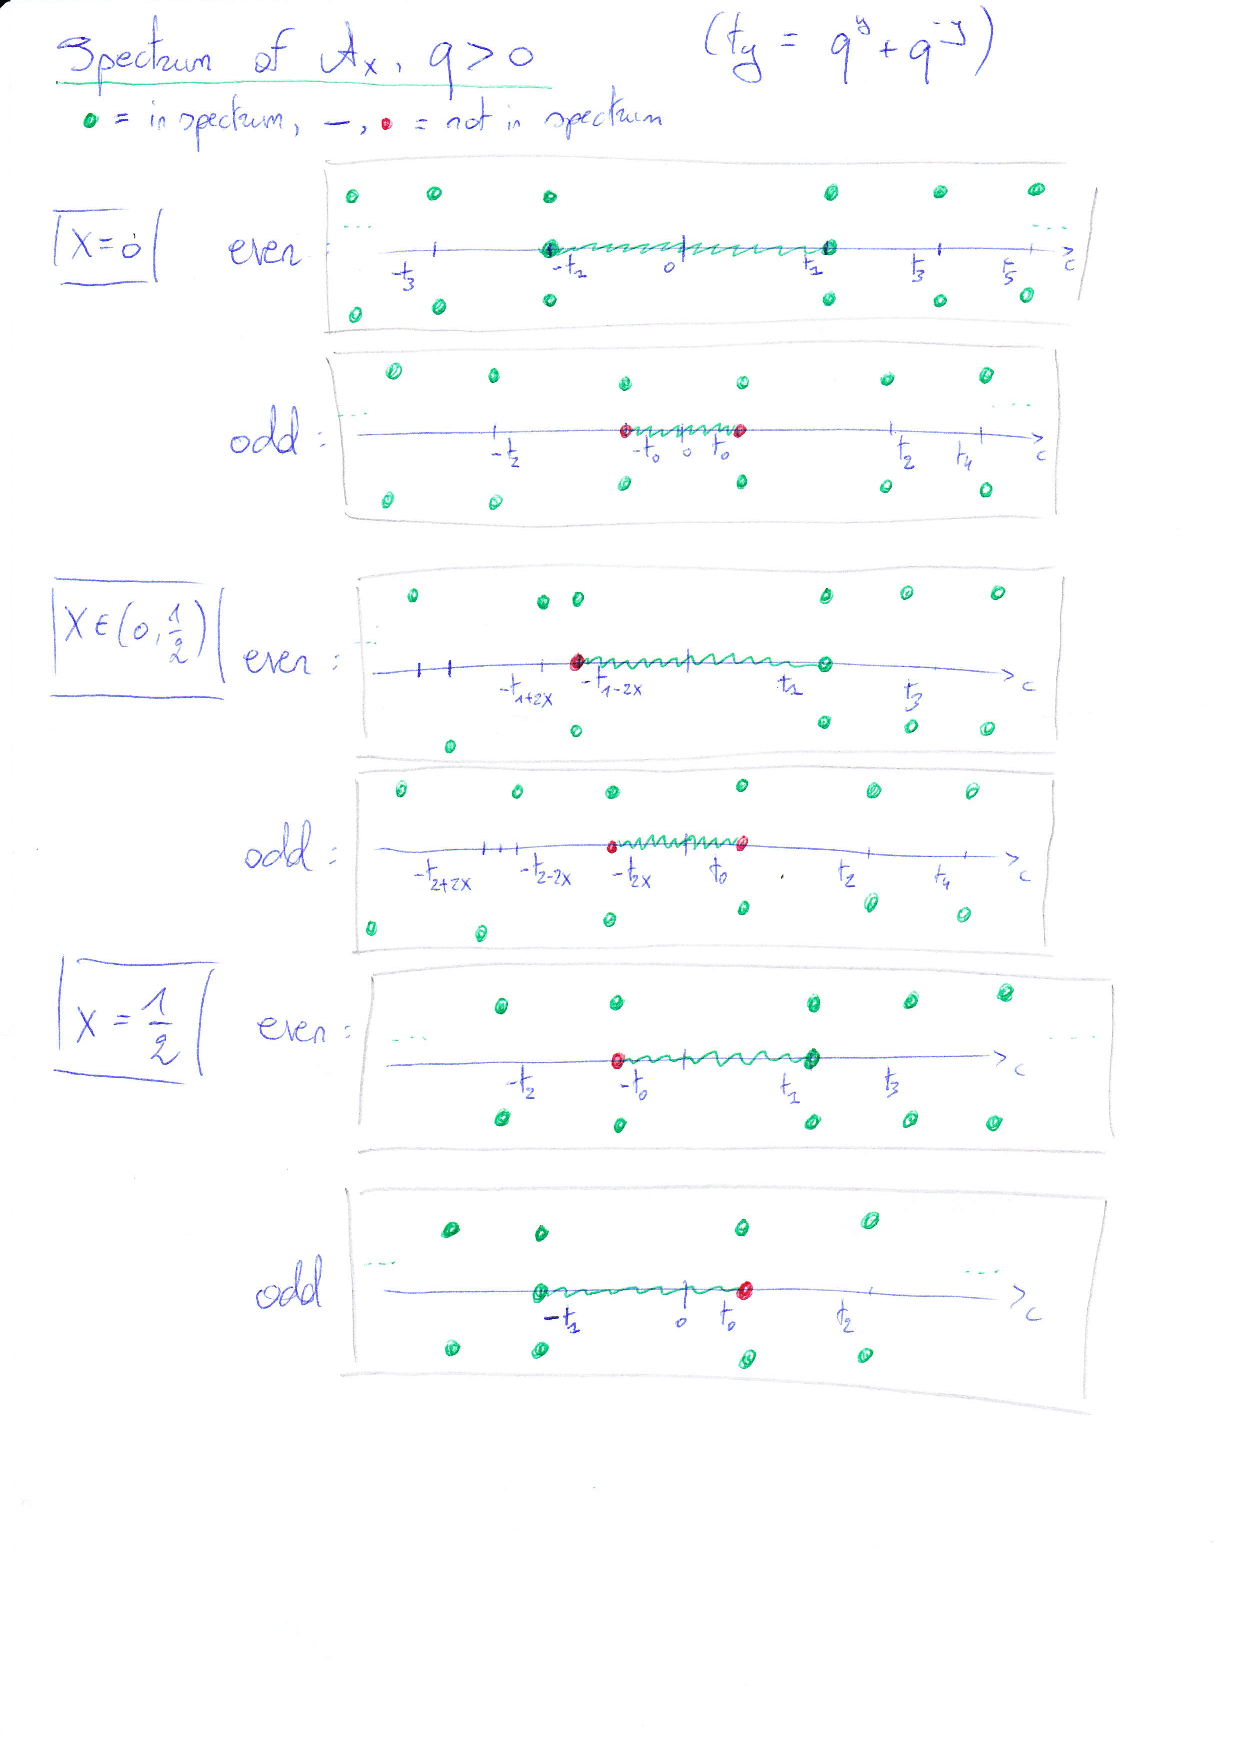
\includepdf[pages={1}]{ScanSpec.pdf}


% Make remark on regular representation cf. Koelink-Rosengren

% Include a concrete descripition of the universal envelope of $A_x$ from this?


%More generally, 

%As a concrete instance of the example of monoidal equivalence, let $\tilde{A}$ be the generalized compact Hopf face algebra obtained from the set $\tilde{I} =I_1\sqcup I_2$ with $I_1= \Z$ and $I_2= \{\bullet\}$ with the $B_{kl} =\emptyset$ and $E(k,l)$ for $k,l\neq \bullet$ as in section ..., with $B_{k,\bullet} = B_{\bullet,k}= \emptyset$, and $B_{\bullet,\bullet} = \{\pm\}$ with $E_{\bullet,\bullet} = \begin{pmatrix} 0 & |q|^{1/2} \\ -\sgn(q)|q|^{-1/2}&0\end{pmatrix}$ (with the basis ordered as $-,+$). Then this will be obtained from the direct sum of the functor from ... and the ordinary forgetful functor from $\Rep(SU_q(2))$ into $\Hilb$. It follows that the components $\tilde{A}(ij)$ can be described by the generators and relations as in ..., but with $F(\lambda)$ and $F(\rho)$ set equal to 1 whenever the corresponding index is $\bullet$.




% Study spectrum fundamental character
% Study dual quantum groupoid
% Make connection with dynamical cocycle
% In case of qgroupoid constructed from identity functor for Rep(SU_q(2)): rep theory of associated Galois object should just be: a single representation (Galois object is type I factor, cutdown of $B(\mathscr{L}^2(SU_q(2)))$). Yes: in general, Galois object is Morita equivalent with algebra of original ergodic action, should also be stressed for Podles spheres





%%% Local Variables: 
%%% mode: latex
%%% TeX-master: "dyn-suq-main"
%%% End: 


\begin{thebibliography}{99}
\bibitem{AN1} N. Andruskiewitsch and S. Natale, Double categories and quantum groupoids, \emph{Publ. Mat. Urug.} \textbf{10}, 11--51 (2005).
\bibitem{BDV1} J. Bichon, A. De Rijdt and S. Vaes, Ergodic coactions with large multiplicity and monoidal equivalence of quantum groups, \emph{Comm. Math. Phys.} \textbf{262} (2006), 703--728.
\bibitem{Boh1}  G. B\"{o}hm, J. Gómez-Torrecillas and E. López-Centella, Weak multiplier bialgebras, \emph{Trans. Amer. Math. Soc.}, in press., arXiv:1306.1466. 
\bibitem{Dau1} J. Dauns, Multiplier rings and primitive ideals, \emph{Trans. Amer. Math. Soc} \textbf{145} (1969), 124--158.
\bibitem{DCY1} K. De Commer and M. Yamashita, Tannaka-Kre\u{\i}n duality for compact quantum homogeneous spaces II. Classification of quantum homogeneous spaces for quantum $SU(2)$, J. Reine Angew. Math., DOI: 10.1515/crelle-2013-0074 (2013).
\bibitem{Eti1} P. Etingof and V. Ostrik, Module categories over representations of $\SSL_q(2)$ and graphs, \emph{Math. Res. Lett.} \textbf{11} (1) (2004), 103--114.
\bibitem{Hay1} T. Hayashi, Compact Quantum Groups of Face Type, \emph{PRIMS} \textbf{32} (1996), 351--369.
\bibitem{KoR1}  E. Koelink and H. Rosengren, Harmonic Analysis on the $SU(2)$ Dynamical Quantum Group, \emph{Acta Applicandae Mathematica} \textbf{69} (2) (2001), 163--220.
\bibitem{Pin2} C. Pinzari, The representation category of the Woronowicz quantum group $S_{\mu}U(d)$ as a braided tensor C$^*$-category, \emph{Int. J. Math.} \textbf{18} (2) (2007), 113--136.
\bibitem{Pin3} C. Pinzari and J.E. Roberts, Ergodic actions of compact quantum groups from solutions of the conjugate equations, preprint (2008) {\tt arXiv:0808.3326 [math.OA]}.
\bibitem{Tur1} V. Turaev, Quantum invariants of knots and 3-manifolds, \emph{de Gruyter Studies in Mathematics} \textbf{18}, Walter de Gruyter \& Co., Berlin (1994).
\bibitem{VDae1} A. Van Daele, Multiplier Hopf algebras, \emph{Trans. Amer. Math. Soc.} \textbf{342} (1994), 917--932.
\bibitem{VDae2} A. Van Daele, An algebraic framework for group duality, \emph{Adv. in Math.} \textbf{140} (1998), 323--366.
\bibitem{VDW2} A. Van Daele and  S. Wang, Weak multiplier Hopf algebras. Preliminaries, motivation and basic examples, \emph{Banach Center Publ.} \textbf{98} (2012), 367--415.
\bibitem{VDW1} A. Van Daele and S. Wang: Weak multiplier Hopf algebras I. The main theory, \emph{Preprint University of Leuven and Southeast University of Nanjing} (2012), to appear in
\emph{Crelles Journal}, {\tt arXiv:math/1210.4395 [math.RA]}.
\bibitem{Yam1} S. Yamagami, A categorical and diagrammatical approach to Temperley--Lieb algebras, preprint (2004) {\tt arXiv:math/0405267 [math.QA]}.
\bibitem{Wor1} S.L. Woronowicz, Twisted $\mathrm{SU}(2)$ group. An example of a non-commutative differential calculus, \emph{Publ. Res. Inst. Math. Sci.} \textbf{23} (1) (1987), 117--181.
\end{thebibliography}

\end{document}

Scraps of section 2 for further ref.

\section{Structure theory for compact quantum groups of face type}


\begin{Def} A \emph{(right) comodule} for a generalized face bialgebra $(A,\Delta)$ over $I$ is an $I^2$-graded vector space $V = \osum{K\in I^2} V(K)$ together with linear maps \[\delta\Grru{K}{L}:V(L)\rightarrow V(K)\otimes A\Grru{K}{L}\] satisfying \[(\id\otimes \Delta\Grru{K}{L})\delta(K*L) = (\delta(K)\otimes \id)\delta(L)\] and \[(\id\otimes \varepsilon_K)\delta\Grru{K}{K} = \id_{V(K)}.\]

We say $(V,\delta)$ is \emph{of finite type} (or simply \emph{finite}) if the support of $M\mapsto V(M)$ is finite in one variable if the other variable is held fixed.% Call this separately finite support? 
\end{Def}

For example, each $\oplus_{L} A\Grru{K}{L}$ is a right comodule under $\Delta$. We will write \[\delta(M)(v) = v_{(0)M_u}\otimes v_{(1)M},\] to be interpreted as zero if $v\notin V(M_u)$.

We have a tensor product $\boxtimes$ on finite comodules by putting \[(V\boxtimes W)(M) = \underset{K\cdot L = M}{\oplus} (V(K)\otimes V(L))\] with comodule structure \[\delta(M)(v\otimes w) = \underset{K\cdot L = M}{\sum} v_{(0)K_u}\otimes w_{(0)L_u} \otimes v_{(1)K}w_{(1)L}.\] We then obtain a tenor category with unit the vector space $\mathbf{1} = \Fun_{\fin}(I)$ of finite support functions on $I$ with grading $\mathbf{1}(k,l) = \delta_{k,l} \C \delta_k$ (with $\delta_k$ the Dirac function at $k$) and comodule structure \[\delta(K,K)(\delta_{K_d}) = \delta_{K_u}\otimes e(K).\]

When $(A,\Delta)$ is a Hopf face algebra, this tensor category admits left % or right - sort out
 duals. Indeed, define $(V^*)(M) = V(M^{\circ})^*$ with coaction \[(\delta(M)(\omega))(v) = \omega(v_{(0)M_d^{\circ}})S(v_{(1)M^{\circ\bullet}}),\qquad \omega\in V(M_d^{\circ})^*,v\in V(M_u^{\circ}).\] Then the natural dualities between the $V(K)$ and $V^*(K^{\circ})$ lead to comodule maps \[\oplus_{K} V^*(K^{\circ})\otimes V(K) \rightarrow \mathbf{1}_K,\qquad \mathbf{1}_K\rightarrow \oplus_K V(K)\otimes V^*(K^{\circ}).\]

%\subsection{Invariant functionals}

Let us now turn to the notion of invariant functional.

\begin{Def} Let $I$ be a set. An \emph{invariant functional} for a Hopf face algebra $(A,\Delta)$ over $I$ is a functional $\varphi:A \rightarrow \C$ such that for all $K,L$ and $a\in A(K*L)$ we have \[(\id\otimes \varphi)\Delta\Grru{K}{L}(a) = \delta_{K_l,K_r}\varphi(a)e(K_l),\qquad (\varphi\otimes \id)\Delta\Grru{K}{L}(a) = \delta_{L_l,L_r} \varphi(a)e(L_r).\] We say that $\varphi$ is normalized if $\varphi(\lambda_k\rho_l)=1$ for all $k,l\in I$ with $\lambda_k\rho_l\neq 0$.
\end{Def}

%\begin{Lem} We have $\varphi(\Gr{A}{k}{l}{m}{n}) = \delta_{k,l}\delta_{m,n}\C$.\end{Lem}

% TODO: make connection with weak multiplier Hopf algebras

\begin{Lem} An invariant normalized functional $\varphi$ is faithful, i.e. $\varphi(ab)=0$ for all $b$ implies $b=0$, and $\varphi(ab)=0$ for all $a$ implies $b=0$.
\end{Lem}

\begin{proof} We follow ad verbatim the proof of Proposition 3.4 in [VDae, Algebraic framework]: if $\varphi(ba)=0$ for all $a$, we arrive at the conclusion that for all $d\in A$ and all functionals $\omega$ on $A$, the element $p = (\omega\otimes \id)((d\otimes 1)\wDelta(a))$ satisfies $(\id\otimes \varphi)((1\otimes c)\wDelta(p)) = 0$. Continuing as in that proof, we obtain from the antipode trick that $\sum_n \varphi(cS(q)\rho_n)\varepsilon(p\lambda_n)=0$. Choosing now for $c$ and $q$ local units of the form $\lambda_k\rho_l$, the normalization condition on $\varphi$ gives that $\varepsilon(p\lambda_n)=0$ for all $n$, hence $\varepsilon(p)=0$. This implies $\omega(da)=0$. As $\omega$ and $d$ were arbitrary, it follows that $a=0$.

The other case follows similarly, considering the opposite algebra.
\end{proof}

% This part is necessary to put into Enock framework, but might possibly be skipped if we only want an operator algebra implementation of dynamical quantum SU(2), as then one has enough with the multiplicative unitaries
Our next aim is to prove that a normalized invariant functional is modular, that is, there exists an automorphism $\sigma: A\rightarrow A$ such that for all $a,b\in A$, we have \[\varphi(ba) = \varphi(a\sigma(b)).\]

\begin{Lem} Let $\varphi$ be a normalized invariant functional. For all $a\in A$ and $k,m\in I$, we have \[\varphi(a\lambda_k) = \varphi(\lambda_ka),\qquad \varphi(a\rho_m) = \varphi(\rho_ma).\]
\end{Lem}

\begin{proof}

\end{proof}



\begin{Def} Define \[V: \osum{n} A_n\otimes {}_{n}A \rightarrow \osum{r} {}_rA\otimes {}^rA\] by the formula \[a\otimes b\rightarrow \wDelta(a)(1\otimes b).\]
\end{Def}

\begin{Lem}\label{LemUni} The map $V$ is an isomorphism.
\end{Lem}
\begin{proof} As $\wDelta(A)(A\otimes A)\subseteq E(A\otimes A)$ with $E = \sum_p \rho_p\otimes \lambda_p$, it is clear that $V$ has the proper range. Define \[\widetilde{V}:  \osum{r} {}_rA\otimes {}^rA\rightarrow\osum{n} A_n\otimes {}_{n}A\] by means of the formula \[a\otimes b \mapsto a_{(1)}\otimes S(a_{(2)})b = a_{(1)}\otimes S(S^{-1}(b)a_{(2)}).\]

By the defining property of $S$, we find that for all $a,b,c\in A$, we have \[(c\otimes 1)\cdot (\widetilde{V}V)(a\otimes b) = \sum_p ca_{(1)}\varepsilon(a_{(2)}\lambda_p)\otimes \rho_pb.\] By the previous lemma, this equals $\sum_p ca_{(1)}\varepsilon(a_{(2)}\rho_p)\otimes \rho_pb$. But as $a\otimes b = \sum_p a\rho_p\otimes \rho_pb$ by assumption, we obtain that \[(c\otimes 1)\cdot (\widetilde{V}V)(a\otimes b) = ca_{(1)}\varepsilon(a_{(2)})\otimes b = ca\otimes b,\] proving that $\widetilde{V}V(a\otimes b) = a\otimes b$.

The identity $V\widetilde{V} = \id$ is proven similarly.
\end{proof}

\begin{Cor} Define \[W: \osum{n} {}_n A \otimes {}^nA  \rightarrow \osum{r} \; {}^rA\otimes A^r\] by the formula \[a\otimes b \rightarrow S^{-1}(b_{(1)})a\otimes d_{(2)} = S^{-1}(S(a)b_{(1)})\otimes b_{(2)}.\] Then $W$ is invertible, its inverse being given as \[W^{-1}(a\otimes b) = \wDelta(b)(a\otimes 1).\]
\end{Cor}

\begin{proof} Apply the previous Lemma to $(A,\Delta^{\op})$.
\end{proof}



\subsection{Generalized compact Hopf face algebras}


A non-degenerate algebra $A$ is called a $^*$-algebra if it comes equipped with an anti-linear involutive anti-homomorphism $A\rightarrow A, a\mapsto a^*$. In this case, $M(A)$ becomes a $^*$-algebra in a natural way. For example, we always consider $\Fun_{\fin}(I)$ as a $^*$-algebra by the ordinary complex conjugation of functions, $f^*(k) = \overline{f(k)}$.




\begin{Def} A couple $(A,\Delta)$ consisting of a generalized Hopf face $^*$-algebra with an invertible antipode invariant normalized functional $\varphi$ is called a \emph{generalized compact face algebra}.
\end{Def}

One proves that a generalized Hopf face $^*$-algebra has $S(S(x)^*)^*=x$ for all $x$, so $S$ is automatically invertible. It then follows by symmetry that also the maps \[(W^{k,t}_{m,n,u,v})^*: \oplus_l \Gr{A}{k}{l}{m}{n} \otimes \Gr{A}{l}{t}{u}{v} \rightarrow \oplus_r \Gr{A}{k}{t}{m}{r}\otimes \Gr{A}{n}{r}{u}{v}\] defined by the formula \[a\otimes b\rightarrow \Delta(b)(a\otimes 1)\] are unitaries, with inverse map $a\otimes b\mapsto S^{-1}(b_{(1)})a\otimes b_{(2)}$.

\begin{Lem}\label{LemUni} Let $(A,\Delta)$ be a generalized compact face algebra. Then each $V^{k,l,s,t}_{m,v}$ is a unitary, and similarly for the $W^{k,t}_{m,n,u,v}$.
\end{Lem}

\begin{proof} It is immediately checked that $V^{k,l,s,t}_{m,v}$ is isometric.
\end{proof}

Let us write $\mathscr{L}^2(A,\varphi)$ for the completion of $A$ with respect to the inner product $\langle a,b\rangle = \varphi(a^*b)$. The canonical inclusion of $A$ into $\mathscr{L}^2(A)$ will be denoted $\Lambda$.

\begin{Lem} Assume $(A,\Delta)$ is a generalized compact face algebra. The representation of $A$ by left multiplication on itself extends to a representation by bounded operators on the completion $\mathscr{L}^2(A,\varphi)$.
\end{Lem}

\begin{proof} Denote $\omega_{\xi,\eta}(x) = \langle \xi,x\eta\rangle$ for $\xi,\eta$ vectors and $x$ a bounded operator. Then a straightforward computation shows that \[(\omega_{\Lambda(a),\Lambda(b)}\otimes \id)(V) = \varphi(a^*b_{(1)})b_{(2)}\] as a left multiplication operator. As $(A\otimes 1)\Delta(A) = (A\otimes A)\Delta(1)$ by Lemma \ref{LemUni} (applied to the opposite algebra), it follows by normalization of $\varphi$ that each element of $A$ can be represented in the form $(\omega_{\Lambda(a),\Lambda(b)}\otimes \id)(V)$, and hence extends to a bounded operator on $\mathscr{L}^2(A,\varphi)$.
\end{proof}

In the following, we will abbreviate $\mathscr{L}^2(A)$ by $L^2A$.

Let $(A,\Delta)$ be a generalized compact face algebra. Denote the von Neumann algebraic completion of $A\subseteq B(L^2A)$ by $M$. Denote $L^2A\iitimes L^2A = E(L^2A\otimes L^2A)$, where $E = \sum_p \rho_p\otimes \lambda_p$ is extended to a bounded operator (in fact, a self-adjoint projection). Finally, denote $M\itimes M = E(M\otimes M)E$. Then $M\itimes M$ is the von Neumann algebraic completion of $A\itimes A$.

Extend now the $V^{k,l,s,t}_{m,v}$ to unitaries \[V: \oplus_p L^2(A_p)\otimes L^2({}_pA) \rightarrow \oplus_p L^2({}_pA)\otimes L^2({}^pA)= E(L^2A\otimes L^2A).\] Then we can construct a map \[\Delta: M\rightarrow M\itimes M,\quad x\rightarrow V(x\otimes 1)V^*.\] By direct computation, we see that $\Delta$ extends the comultiplication map on $A$. It is then immediate to check that $\Delta$ is in fact coassociative (where one may as well consider $\Delta$ as a non-unital map from $M$ to $M\otimes M$).

We aim to show that $(M,\Delta)$ can be fitted into the theory of measured quantum groupoids.

%%%%%%%%%%%%%%%%%%%%%%%%%%%%%%%%%%%%

Remnants of section 6


\subsection{Representation theory of the intertwiner function algebra on the dynamical quantum $SU(2)$ group (to be modified)}

\begin{Lem} There are faithful $^*$-representations $\pi_{\pm}$ of $\Pol_{\ext}(\X)$ as operators $\mathscr{D}^{\pm}\rightarrow \mathscr{D}^{\pm}$, given by the following formulas (where we suppress the explicit notations $\pi_{\pm}$): \begin{align*} \alpha\cdot e_{n,y}^+ = \left(\frac{1+q^{2n-2y}}{1+q^{-2y-2}}\right)^{1/2}e_{n,y+1}^+,&& \beta\cdot e_{n,y}^+ = \left(\frac{q^{-2y}-q^{2n-2y+2}}{1+q^{-2y-2}}\right)^{1/2}e_{n+1,y+1}^+,\end{align*}
\begin{align*} \alpha\cdot e_{n,y}^- = \left(\frac{1-q^{2n}}{1+q^{-2y-2}}\right)^{1/2}e_{n-1,y+1}^-,&& \beta\cdot e_{n,y}^- = \left(\frac{q^{2n+2}+q^{-2y}}{1+q^{-2y-2}}\right)^{1/2}e_{n,y+1}^-,\end{align*} the functions in $C_c(\R)$ simply acting by $fe_{n,y}^{\pm}= f(y)e_{n,y}^{\pm}$.

Both representations are bounded when restricted to $\Pol(\X)$.
\end{Lem}

%Miyashita Ulbrich?


%\section*{Representation theory of the dynamical quantum $SU(2)$ group}

%We let $A$ be the universal $^*$-algebra generated by the elements of a unitary $U = \begin{pmatrix} a & b \\ c & d\end{pmatrix}$ and a copy of $l^{\infty}(\Z\times \Z)$ such that \begin{eqnarray*} d^* &=& \frac{Z(\lambda)}{Z(\rho)}a ,\\ c^* &=& -\sgn(q)  Z(\lambda)Z(\rho-1),\end{eqnarray*} where $Z(k) = \left(\frac{|q|^{x+k}+|q|^{-x-k}}{|q|^{x+k+1}+|q|^{-x-k-1}}\right)^{1/2}$. We look for irreducible representations of $A$ such that the restriction to $c_c(\Z\times \Z)$ is non-degenerate. 
%We write $\beta = qF(\rho)^{1/2}u^{-,+}$, where $F(k) = |q|^{-1}Z(k)^{-2}$.

%Let \[\Omega = |q|^{\lambda-\rho+1}+|q|^{\rho-\lambda-1}-(|q|^{x+\lambda+1}+|q|^{-x-\lambda-1})(|q|^{x+\rho}+|q|^{-x-\rho})b^*b\] which we consider as a formal element. Then $\Omega$ is central. Since in any non-degenerate representation $\pi$ of $A$ the Hilbert space $\Hsp$ decomposes into direct summands $\Hsp_{k,l}$, the action of $\Omega$ on the algebraic direct sum of all $\Hsp_{k,l}$ is meaningful. If then $\pi$ is irreducible, it is clear that $\pi(\Omega)$ must be a scalar.


\subsection{Representation theory of the function algebra on the dynamical quantum $SU(2)$ group}


% Study spectrum fundamental character
% Study dual quantum groupoid
% Make connection with dynamical cocycle
% In case of qgroupoid constructed from identity functor for Rep(SU_q(2)): rep theory of associated Galois object should just be: a single representation (Galois object is type I factor, cutdown of $B(\mathscr{L}^2(SU_q(2)))$). Yes: in general, Galois object is Morita equivalent with algebra of original ergodic action, should also be stressed for Podles spheres

\begin{Lem} There are faithful $^*$-representations $\pi_{\pm}$ of $\Pol_{\ext}(\X)$ as operators $\mathscr{D}^{\pm}\rightarrow \mathscr{D}^{\pm}$, given by the following formulas (where we suppress the explicit notations $\pi_{\pm}$): \begin{align*} \alpha\cdot e_{n,y}^+ = \left(\frac{1+q^{2n-2y}}{1+q^{-2y-2}}\right)^{1/2}e_{n,y+1}^+,&& \beta\cdot e_{n,y}^+ = \left(\frac{q^{-2y}-q^{2n-2y+2}}{1+q^{-2y-2}}\right)^{1/2}e_{n+1,y+1}^+,\end{align*}
\begin{align*} \alpha\cdot e_{n,y}^- = \left(\frac{1-q^{2n}}{1+q^{-2y-2}}\right)^{1/2}e_{n-1,y+1}^-,&& \beta\cdot e_{n,y}^- = \left(\frac{q^{2n+2}+q^{-2y}}{1+q^{-2y-2}}\right)^{1/2}e_{n,y+1}^-,\end{align*} the functions in $C_c(\R)$ simply acting by $fe_{n,y}^{\pm}= f(y)e_{n,y}^{\pm}$.

Both representations are bounded when restricted to $\Pol(\X)$.
\end{Lem}

